\documentclass[a4paper]{report}

\usepackage[square, numbers]{natbib}
\usepackage{hyperref}
\usepackage{url}
\usepackage{graphicx}
\usepackage{tabularx}
\usepackage{caption}
\usepackage{subcaption}
\usepackage[english]{babel}
\usepackage{enumitem}
\usepackage{array}
\usepackage{lscape}
\usepackage{gensymb}
\usepackage{pbox}
\usepackage{nameref}
\usepackage[chapter]{algorithm}
\usepackage{algorithmicx}
\usepackage{algpseudocode}
\usepackage{geometry}
\usepackage{float}
%\restylefloat{table}
 \geometry{
 a4paper,
 total={210mm,297mm},
 left=30mm,
 right=30mm,
 top=15mm,
 bottom=15mm,
 }


% Title Page
\title{Software Design Study\\Final Report}
\author{Jack Browne, 1236782\\Thomas Clarke, 1162927\\Keiran Crook, 1257447}


\begin{document}
\maketitle

\tableofcontents

\chapter{Introduction}
\section{Problem Definition}
%Rest of page on why we chose this problem space
%Key statistics
We began this project by exploring the `Safety in Cycling' problem space. Our motivation for exploring this space came from looking at the reasons why people do not cycle. Even though cycling is a fairly easy form of exercise and an environmentally friendly method of transport just 2\% of trips are made by bicycle\cite{travelsurvey}. We feel that this figure is way too low and should probably be closer to the 10\% mark to bring the UK in line with the rest of Europe.

Investigating this, we looked at some of the reasons why people choose not to cycle in the UK and the general trend was that people thought cycling was not safe enough. For example, a question in a Transport for Greater Manchester survey asked ``Which of the following do you feel are the barriers to cycling?" and 74\% of respondents said `Road Safety'\cite{TfGM}. In a similar survey by the Department for Transport 61\% of people either definitely agreed or tended to agree with the statement ``It is too dangerous for me to cycle on the roads"\cite{dft}.

In fact, interestingly, when comparing fatalities there is actually more risk being a pedestrian than a cyclist. This may be evidence that the problem is more about `subjective safety' rather than absolute risk. 

Safety is quite a wide term so we had to speak to different stakeholders and analyse some statistics to really see the reasons \textit{why} cycling is not safe (or at least not considered to be safe). From this research we were able to narrow the problem down to the following:

\begin{itemize}
  \item Reducing the number of accidents on UK roads, with a particular focus on commuting hours. The majority of accidents occur during these hours; likely because of the increased traffic causing car drivers to become frustrated and/or make mistakes. 
  \item Improving the perception of cycling to be a safe mode of transport. This is to address the `subjective safety' issue. A successful solution to this should not only make the cycling safer but the safety improvement should be clear and obvious to the cyclist themselves. We believe that this is reason why, although accident numbers are falling, current safety products have not seen the number of cyclists dramatically increase.
\end{itemize}
%Maybe this section can go
\section{Purpose}
This report is written for the benefit of any software or hardware engineers who are tasked with implementing this product. For this reason, in parts, the report may assume some basic technical knowledge of these fields. For example, understanding of the UML diagrams used in section ?.

The report should describe, in detail, our solution to the problem above. The detail should be enough so as that a small team of people would be able to implement the solution in its entirety with relative ease. The report should address all of they key areas of the solution and be void of any ambiguities so that it alone can clarify any queries about the product.

As well as this, the report will show the progression of our ideas and the steps taken to reach our final design. Throughout the design of this product we reached points where we had to make a justified decision from a range of possibilities. We always tried to make a rational decision based on the information available coupled with our in-depth knowledge of the problem space. Each of these key decisions will be described in detail for the benefit of the reader.

\section{Overview}
Firstly this report will give a rough outline of the solution that we came up with and why we decided to go with that particular solution as well as some of the features we considered but ultimately decided not to include. This will help to give some context to sections of the report that follow.

Before discussing the details of the design we will outline some of the things we had to take into consideration before designing our solution. Including the overall design goals that we were following throughout.

In the later sections of the report we will describe in detail the overall architecture of the product and how the main components of the system will work. Many of these components are either amalgamations of the best features of the similar products on the market or involved a choice between different ideas. For all of these cases we will describe in some detail all of the different options that we had and then our reasons for choosing a particular one over another.

Finally we will present our critical analysis of the prototypes that we created and show how using this analysis we iterated on the prototypes to reach to our final design.

\section{Definitions, Acronyms and Abbreviations}
\begin{description}
\item[RTA] Road Traffic Accident
\item[UCI] Union Cycliste Internationale
\item[I/O] Input/Output
\item[RAM] Random Access Memory
\end{description}
\section{References}
The design decisions that we made are based on our earlier research and we will continually refer to this research throughout the report, all of which is documented in the Research Report found in the appendix. 

All other papers, articles, etc. that were used to formulate our ideas are referenced in the Bibliography.

\chapter{System Overview}
% 2 or 3 pages on what the finished syetem does
% Intended users
% Key features and why
% Rejected features and why
After fully analysing the problem space we came up with an idea for a product that we felt solved the key issues around bike safety. As with most modern products, ours is heavily influenced by new technologies; particularly automation systems in cars culminating in the recent development of self-driving cars. % Reference Google project

The core of our product is a collision avoidance system revolving around automated braking. In general the bike should be capable of analysing other road users, predicting the likelihood of a collision occurring and then applying the necessary amount of braking. The technology for performing this task in cars is fairly well developed and becoming more and more widely deployed, for example the Subaru EyeSight\cite{eyesight} and a similar system developed by Volvo\cite{volvo}. However there is no such system for road bikes. This is probably due to the computing power needed and a bikes natural instability. We believe that these problems can be overcome with some careful design.

We decided this should be a fully integrated bicycle rather than a set of accessories for somebodies existing bike. The primary reason for this is to help overcome the instability issue. An additional reason is that it allows us to incorporate a wider range of sensors than would be feasibly possible in an accessory kit. This does have the disadvantage that some people may have already spent a large sum of money on their current bike and may not want to part with it.


To interface this system there will be a smartphone application, enabling users to customise their settings and have them automatically download whenever they get on the bike. As well as this, the smartphone app will provide some performance information to the user as they are cycling such as current speed and the current battery level of the bike.

\section{Rejected features}
During our research we discussed a multitude of different solutions (or parts of solutions); some of which were very similar to our final design and some which are markedly different. Many of these solutions were rejected reasonably quickly while others were still being discussed during later iterations of the design. However all of the ideas below were eventually rejected because they were either unsuitable or unnecessary.

\paragraph{Safety based route planner} \label{subsec:rejected} An idea that was considered for a long time was a route planning application. This was intended to work alongside the collision avoidance system as part of an wider ecosystem of safety technologies. Core to this would be crowdsourcing information from all other road users; traffic speeds, accidents, road conditions, etc.. All of this information could then be combined and analysed in order to provide the cyclist with the safest route. We deemed the safest route to be: 
\begin{enumerate}
\item One with less traffic, as discovered from research [enter research], there was a positive correlation between increased traffic and increased cyclist accidents. 
\item One which avoided areas with a certain risk level, both short and long term. A known accident blackspot might be a long term risk. If an accident has just occurred then the surrounding area might be a short term risk.
\item One which took environment factors into consideration, that were deemed a risk to cyclist. For example poor road conditions, poor weather conditions, high pedestrian activity, etc.
\end{enumerate}
 
This was an idea that we invested a lot of time into and one that we still believe under the right conditions could be very successful. However, for our project we decided to drop this feature because:
\begin{itemize}
\item It was too dependent on other users to enable it to offer what we wanted. Car drivers needed to use the application and we did not think enough drivers would be willing to share all of the necessary information for something that provides them with little benefit.
\item It would require too many sensors and additional components for it to be a viable option. This could be overcome by having it as part of an integrated bicycle however in this case we would likely not have the required number of users for it to be successful.
\end{itemize}


\paragraph{Wearable tech}As a group we very quickly latched onto the idea of incorporating wearable technology into our final solution - particularly inspired by recently evolving wearable eyewear technology such as Google Glass. We felt that one of the problems we would eventually have is that a bike has no significant interface/dashboard and wearable eyewear is a very natural solution to this problem. The other interface solutions that we came across were: 
\begin{itemize}
  \item a smartphone mounted on the handlebars
  \item a small on-board-computer
  \item more recently, smartwatches
\end{itemize}
However all of these have the same fundamental problem; they require the cyclist to divert their attention away from the road. Lack of attention, from either party, is one of main causes of RTAs involving bicycles. %statistic!

In spite of all this we decided to forget this idea following a user-review. Several of the people failed to grasp the concept. Firstly not many people have access to any wearable eyewear technology at present so designing an integrated bike along with an app for an existing eyewear platform is not really feasible. The other alternative would be to design a piece of eyewear technology to use for along with any existing bike however the number sensors that would need to be installed and calibrated means that for most people this simply isn't practical.

\paragraph{Self inflating tyres} An idea that was briefly considered was self inflating tyres. Inspired by similar technology in cars where the tyres will inflate or deflate depending on the current speed or road conditions. Following our research we found that a vaguely similar technology for bikes is currently in development by a San Francisco company PumpTires\cite{pumptyres}. This technology looked promising and even made it into our first prototype.

However, a handful of users asked some interesting questions about this feature which after some consideration prompted us to drop it. When really considering what this feature adds to the overall system we realised that it doesn't really contribute much but drives up the cost vastly. The core of our system is the collision avoidance; self inflating tyres don't really help us to achieve that and in reality this was just a leftover feature from earlier discussion.

As well as this we realised that we had not properly thought through how to actually implement this. PumpTires have patented much of their technology and we don't really have the technical expertise required to invent a new solution. It is possible that we would be able to use PumpTires system directly, however it would be just as easy for people to do this themselves if this is a particularly important issue to them.

\chapter{Design Considerations}
\section{Assumptions}
% 2 pages on the above
% Assumptions about users (age, race, gender, disability)
% Assumptions about environment (road, many other users, etc.)
% Assumptions about interface (All users will have a phone)
% Constraints (Cost, weight/size)
When designing this system we have had to make a few assumptions about certain characteristics of the end users, this is because it would be almost impossible to design a system of this nature that is both effective and easy for everybody to use. 

Firstly we have assumed that the end user will be fully able-bodied. We feel that this is a necessary assumption despite the fact that one in twenty cycling commuters are disabled \citep{census-dis}. Cycling is a very physical activity and generally those with severe physical disabilities are better off with a bike that is specifically designed to cater for their particular disability. It is very much possible that our final design will be usable for the less severely disabled, however we will not be creating our design with any of these disabilities in mind. 

Secondly we will be assuming that end users have some familiarity of bikes, particularly road bikes. By this we mean that we will not be designing an educational tool that teaches people how to ride a bike nor an assistance tool that aids those who cannot already ride a bike. This is a reasonable assumption because it would be against recommended practice for a non-cyclist to start out by cycling on main roads anyway. %Who's recommended practice? Sources?
In fitting with both of the above assumptions, we will also be assuming that the bike is to be used only by fully grown adults.

The majority of our research has been based around cycling in the UK for two reasons:
\begin{enumerate}
  \item We are based in the UK, giving us much easier access to end-users (UK cyclists)
  \item Although we didn't look too deeply, our research suggested that many European countries actually have a fairly good cycling population
\end{enumerate} 
Because of this our product will be designed to be used on UK roads. We will make no further assumptions about the environment it is used in. The final product should function on busy city roads, country lanes or quiet residential roads with the same effectiveness. We will not be designing the product to work with any other system of roads (European, American, etc.) but it is highly likely that with some minor adaptations this product could function on any road system.

The final assumption we had to make came about as the result of a discussion following our initial prototype. We assumed that all of our users would have a smartphone. The reasons for making this assumption are discussed in detail in section \ref{sec:phones}. We feel that this was a reasonable assumption because there are an estimated 37.8 million smartphone users in the UK\cite{smartphones}. This is a huge percentage of the adult population that we are aiming at.

\section{Constraints}
There are some overall restrictions that the product naturally has in order for it to be feasible or usable. The main two that we considered were:
\begin{itemize}
  \item \textbf{Cost} because in order for a solution to be considered suitable it must be available to the general population of commuting cyclists. A solution that does everything that we set out to achieve but could never be purchased by even the richest of cyclists could not be considered suitable.
  \item \textbf{Weight} because this has a significant impact on whether the bike is actually ridable. We want to design a solution for which it is, not only possible but, comfortable to ride on the majority of commuting roads. Some of which will involve steep inclines.  
\end{itemize}
\subsection{Cost}
We are attempting to create a solution for the average commuting cyclist to use on the road. This means it is important that the average commuting person is able to afford the product. To do this we must be able to find the right components and produce the bike for a reasonable cost. To decide what constitutes `reasonable' we analysed how much cyclists currently spend on their bikes and asked cyclists how much they would be willing to spend on a bike of this style/quality.
\begin{figure}
\centering
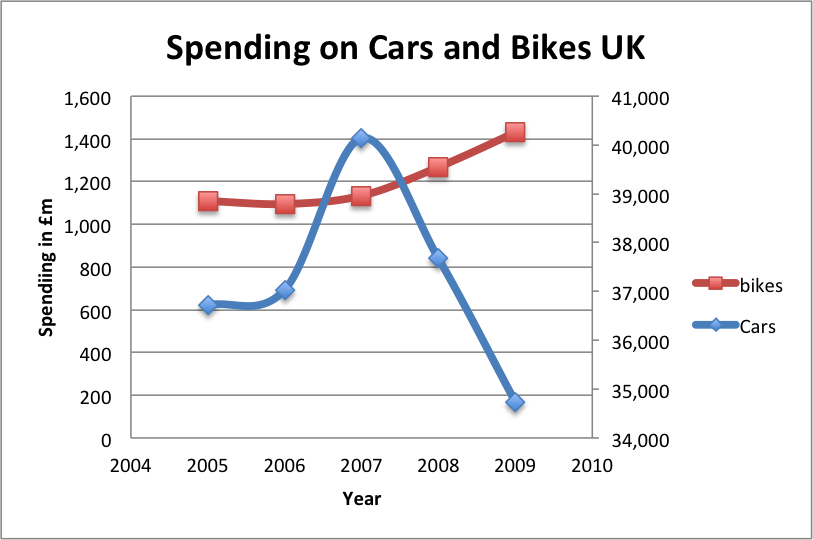
\includegraphics[scale=0.9]{figures/cars-bikes-spending}
\caption{Graph showing the retail sales of cars and bikes \cite{uk-stats}}
\label{fig:cars_bikes_spending}
\end{figure}
\paragraph{Current spending}
Overall spending on bikes is slowly increasing at the same time as spending on cars rapidly decreasing as shown by figure \ref{fig:cars_bikes_spending}.Possibly indicating a   However, last year in the UK, the average amount a person spends on buying a bike was only £233. However, this statistic is likely skewed by the large amount of cheap bikes sold to casual cyclists; these are not the people we are aiming this product towards\cite{spending-more}. There are no readily available statistics that differentiate between the spending on road bikes and otherwise but we were able to get a fairly good idea using statistics from the Cycle to Work scheme - which allows people to buy commuting bikes and equipment tax free. This saw commuters spending an average of over £1,100\cite{spending-more}. This is more in line with the price our bike would retail for and the cyclists we are aiming at. As well as this, our earlier research found that commuters spend a further £195 on accessories alone, many of which may be incorporated directly into our design.

\begin{figure}
\centering
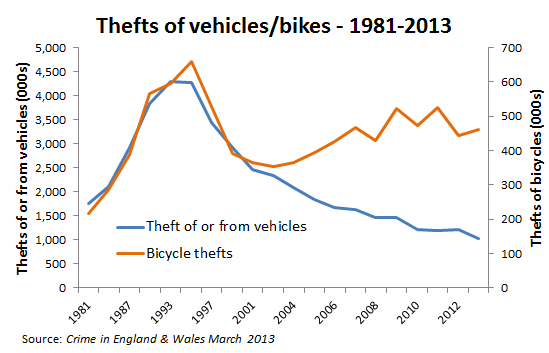
\includegraphics[scale=0.8]{figures/cycle-theft}
\caption{Graph showing the thefts of vehicles and bikes \cite{ctc-stats}}
\label{fig:theft_graph}
\end{figure}
\paragraph{Concerns}
As can be expected; cyclists are always concerned about the theft of their bike. Strangely, thefts of or from cars and other vehicles has been steadily decreasing since the late 90s. While in that time thefts of bicycles has generally increased (Fig. \ref{fig:theft_graph}). This is a worrying trend and may be a contributing factor to people opting for cheaper bikes.

However, we can reasonably assume that consumers who spend more on their products will be  willing to spend a little extra on security or insurance. This might go some way to counteracting the concern about theft. Another way to alleviate these concerns might be to incorporate anti-theft devices into the product itself, similarly to ‘Find my iPhone’ and similar products.
\paragraph{Conclusion}
From the research we decided that an appropriate cost for producing this bike is \pounds1000. Even though this is significantly more than the average spend for a bike we feel that it is justified for a product of this quality since it is in the region that cycling commuters currently spend (particularly once accessories are taken into account). Also, this still comes at considerably less cost than many of the commuting alternatives (driving, public transport,etc).

\subsection{Weight}
There are not many statistics out there regarding the weight of consumer bicycles so most of this research came from talking to cyclists and cycle shops.
\paragraph{Current products}
UCI impose a minimum weight of 15 lbs, for this reason many cyclists consider anything around this weight or lighter to be a \textit{light} bike. However, the retailers that we spoke to were generally of the opinion that bikes at this end of the scale were only really appropriate for competitive racing environments. They thought that 23 lbs was a good weight for a road bike or 30 lbs for a more general purpose mountain bike. These weights give a good trade off between speed and ease of ride.

\paragraph{Electric bikes}
Working with the 23 lb ballpark figure, as suggested by the cycling retailers that we spoke to, we noticed a problem. Given that this product heavily relies on a computer performing some calculations and some sensors feeding information into the computer we clearly will require some sort of battery. Looking at the current bike batteries on the market this would not be easy to fit into our 23 lb restriction. In the Specialized Turbo S, for example, the battery alone weighs 8 lbs\cite{turbo-s}. This would take up over $ \frac{1}{3} $ of our weight limit. This doesn't leave much room for a frame, wheels and pedals; let alone sensors and a computer. When all of this is factored in, we are realistically looking at a minimum of 45/50 lbs. This is likely to be almost to twice the weight that many cyclists are used to and as a result may be very difficult to ride. The obvious solution to this problem is to heavily assist the cyclist with a motor powering the wheels. This is the primary use case for current electric bikes so the technology already exists and shouldn't be too difficult to implement

\paragraph{Conclusion}
Cyclists have a reputation for being obsessed with weight - trying to shave off pounds at every opportunity. However our research showed that most commuters probably wouldn't be overly concerned about a slight increase in weight if it meant an equally good (or better) performance and a more comfortable ride. This makes sense because, in reality, the cyclists themselves are usually by far the biggest contributor to the weight of the bike. Also, as a result of this research, it is likely that our final product will need contain some form of motor or other electronic assistance which will help to carry some of the weight. This puts our product more in line with electric bikes on the market, rather than regular road bikes. This gives some additional flexibility regarding the weight of the bike.

In conclusion we have decided that we will design the bike with a 60 lb restriction. This should allow us to include all of the hardware components that will be necessary for our solution, with the bike still being comfortable to ride. 

\section{Design Goals and Guidelines}
% 1 page on U(X/C)D and why this is suitable for our product
% Double diamond model (Design council)
\subsection{User Centred Design}
Our overall design goal was to come up with a product that was tailored to fit the needs of the end-user. In this case the end-users are cyclists (or potential cyclists). This was especially important for us because the whole idea was to design a product to make cyclists feel safe on the roads. In the User Centred Design process the end-user is involved at every single stage; we continually used the user opinions to formulate or improve our design.

A further consideration was the other stakeholders (a map of which can be found in appendix \ref{ch:stakeholders}). We had to consider these stakeholders as much as possible, for example car drivers might be able to offer some insight that cyclists cannot. It is not possible to get in touch with all of these stakeholders; we could not find anyone that openly admitted to being a bike thief for example.

Some of the User Centred Design methods that we used were:
\begin{description}
  \item[Questionnaires] This was our primary method for getting in touch with users. This was suitable for us because they are relatively cheap and easy to set up. Also cyclists are fairly easy to access which meant we had a large enough sample size to make the information from the questionnaires viable. Questionnaires are particularly good at getting statistical data. This was used predominantly in the requirements gathering stage however some smaller questionnaires were used to allow our user testers to give their feedback on our prototypes.
  \item[Interviews] We carried out a couple of informal interviews with a cycling retailer (Urban Cycles on the university campus). This was a suitable way for us to get in touch with retailers because the number of retailers we were able to talk to was fairly low. 
  Interviews gave us a qualitative opinion on a range of topics. This was good for us because we used these interviews to find out the latest trends and to get expert opinions. Interviews were predominantly used in the requirements gathering and early stages of the design phase.
  \item[Usability testing] We did some usability testing with end users to evaluate our prototypes. We asked people to perform some tasks using our prototype and recorded the time taken. This gave us a statistical measure of how efficient our design was. 
  
  We also watched them as they carried out the task to get a qualitative understanding of the particularly complex areas of the design. This was an evaluation technique.
\end{description}

\subsection{Double Diamond Model}
During this project we followed the Double Diamond design process as put forward by the Design Council\cite{doublediamond}. 

This process has four key stages:
\begin{description}
\item[Discover] In this stage we explored all elements of the problem space; gathering as much information as possible from a whole variety of sources. Statistics were used to give us the raw quantitative data that would be used to back up our views about the problem space, while questionnaires were used to get a more qualitative view. Also questionnaires gave us the opportunity to get opinions directly from potential users (or other stakeholders) of the system; helping the to achieve our goal of creating a user centred design.
\item[Define] Once we had gathered all of our information we then had to interpret it to accurately identify the contributing factors to cycling accidents, allowing us to focus our efforts in the right way. At this stage we also came up with a starting point for final product.
\item[Develop] It was during the development stage that we really investigated all of the different ways of achieving what we had envisaged. Here we had to consider what would be practical, how different components would interact and, most importantly, what actually works.
\item[Deliver] This stage was a series of prototype-feedback loops. We would come up with a prototype, scrutinise it for potential design flaws, adapt the design and repeat. This process continued up until the point where we had our final design.
\end{description}

\begin{figure}[t!]
\centering
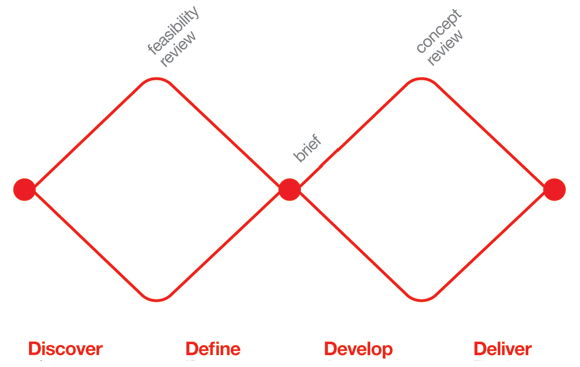
\includegraphics[scale=0.4]{figures/diamond}
\caption{A visual representation of the double diamond model}
\label{fig:diamond}

\end{figure}
\subsection{Agile approach}
We came up with a initial set of requirements during the define stage of the double diamond model - once we had our rough outline of how our solution would work. However these were very open to change. In keeping with our overall goal of creating a user centred design, we allowed the user feedback and prototype analysis to govern how the requirements of the product adapted and changed. 

In an agile approach such as this one the design is developed in small increments - starting from the `minimum viable product' all the way up to the final design. An example of this is how we adapted our prototypes in chapter \ref{ch: prototype}. Without using an agile approach we would not have been able to go back and make these drastic changes to our design because they would most likely conflict with the initial requirements. The agile approach works very nicely within the User Centred Design guidelines.

\chapter{Specification}
In keeping with the agile approach that we took to the design the functional requirements are fairly high level and lacking in detail. This detail was realised in the use cases, shown in section \ref{sec:use-cases}.
\section{Functional Requirements}
\label{sec:func_req}
\begin{enumerate}[label=\ref*{sec:func_req}.\arabic*.,leftmargin=*]
\item The system must be able to detect potential collisions on the road around the user
\begin{description}
\item[Description] The system detects vehicles (possibly pedestrians, too), tracks them and predicts their future trajectory from their velocity, yaw, etc.
\item[Reason] To enable the system to take the appropriate action
\end{description}

\item The system must be able to take some action to prevent the collision from happening
\begin{description}
\item[Description] If a predicted trajectory will cause a collision, then the cyclist is either warned or the system takes over.
\item[Reason] A humans reaction time can place them at risk.
\item[Dependencies] 4.1.1
\end{description}

\item The system must provide notifications to the user
\begin{description}
\item[Description] The system must notify the user about what is going on with the system
\item[Reason] Will make it much easier to use
\item[Dependencies] 4.1.2
\end{description}

\item The system should be lockable remotely
\begin{description}
\item[Description] The user should be able to prevent unwanted access to their bike via a remote device
\item[Reason] To reduce the risk of the bicycle being stolen.
\end{description}

\item The system should allow the user to monitor their cycling performance
\begin{description}
\item[Description] The system should contain some sort of interface for monitoring some statistics such as current speed, etc.
\item[Reason] Cyclists have different cycling methods.
\end{description}

\item The system could monitor tyre pressure
\begin{description}
\item[Description] It would be ideal if the system could keep a real-time view on the pressure in both bicycle tires and present information to the user. If the tires are below a certain pressure, the system must automatically inflate the tires to an optimal pressure
\item[Reason] Deflated tires affects cycling performance and also may damage the bicycle. Automatic inflation will improve the cyclists confidence to cycle
\end{description}
\end{enumerate}

\section{Non-functional Requirements}
\subsection{Usability}
\label{usability}
\begin{enumerate}[label=\ref*{usability}.\arabic*.,leftmargin=*]
\item The system should be easy to use
\begin{enumerate}[label*=\arabic*.]
\item The user should be able to customise the system behaviour easily
\item The system should give appropriate error messages when necessary
\end{enumerate}
\end{enumerate}
\subsection{Efficiency}
\label{efficiency}
\begin{enumerate}[label=\ref*{efficiency}.\arabic*.,leftmargin=*]
\item All elements of the system should load within 1 second
\end{enumerate}
\subsection{Dependability}
\label{dependability}
\begin{enumerate}[label=\ref*{dependability}.\arabic*.,leftmargin=*]
\item The system should be available at all times
\begin{enumerate}[label*=\arabic*.]
\item The core of the system be usable without an internet connection
\end{enumerate}
\end{enumerate}
\subsection{Security}
\label{security}
\begin{enumerate}[label=\ref*{security}.\arabic*.,leftmargin=*]
\item The system should hold all customer information securely
\item The system should be secure from theft
\item The system should be secure from hackers
\end{enumerate}
\subsection{Environmental}
\label{environmental}
\begin{enumerate}[label=\ref*{environmental}.\arabic*.,leftmargin=*]
\item The system should be environmentally friendly
\end{enumerate}
\subsection{Operational}
\label{operational}
\begin{enumerate}[label=\ref*{operational}.\arabic*.,leftmargin=*]
\item The system should be suitable for people aged 16 and over
\end{enumerate}
\subsection{Development}
\label{development}
\begin{enumerate}[label=\ref*{development}.\arabic*.,leftmargin=*]
\item The system should be well documented
\begin{enumerate}[label*=\arabic*.]
\item All code should be properly commented
\end{enumerate}
\end{enumerate}
\subsection{Regulatory}
\label{regulatory}
\begin{enumerate}[label=\ref*{regulatory}.\arabic*.,leftmargin=*]
\item The system should conform to the Pedal Bicycles Safety Regulations (PBSR)
\item The system should comply with Statutory Instrument No. 1168 (1983)
\end{enumerate}
\subsection{Ethical}
\label{ethical}
\begin{enumerate}[label=\ref*{ethical}.\arabic*.,leftmargin=*]
\item The system should not promote bad cycling habits
\end{enumerate}
\subsection{Legislative}
\label{legislative}
\begin{enumerate}[label=\ref*{legislative}.\arabic*.,leftmargin=*]
\item The system should comply with the Data Protection Act 1998
\end{enumerate}

\section{Use cases}
\label{sec:use-cases}

\begin{figure}[h]
\centering
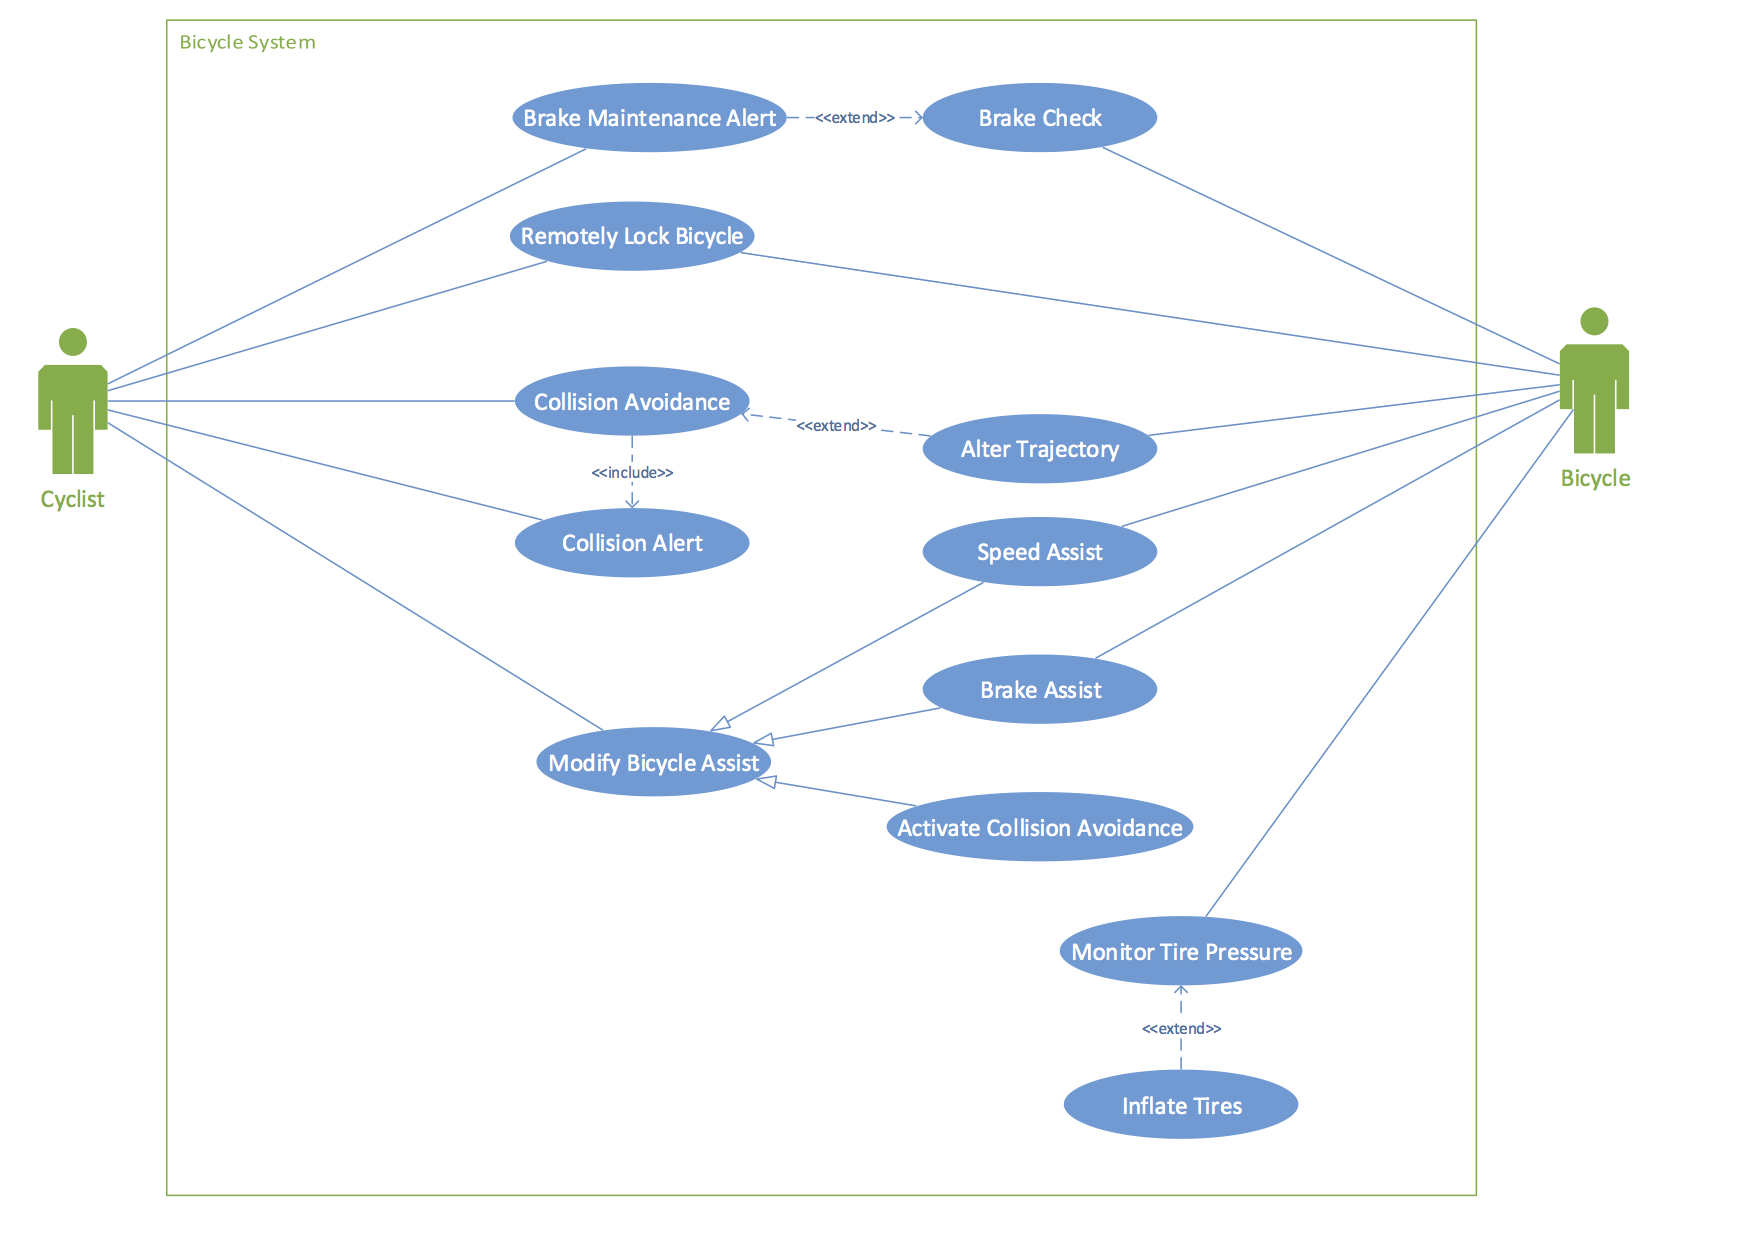
\includegraphics[scale=0.5]{figures/bicycle_system_use_case}
\caption{Use case diagram showing basic expected use cases}
\label{fig:ebicycle_system_use_case}
\end{figure}
\noindent\textbf{Use Case:} Create account \\
\textbf{Description:} If the user does not have an account with the system, the user can create an account using the mobile application \\
\textbf{Preconditions:} \begin{itemize}
\item The user has access to the mobile application
\end{itemize}
\textbf{Flow of events:} \begin{enumerate}
\item The system requests email and password for the new account
\item The user inputs their email and password for the new account
\item The system checks an account under the same email has not already been made
\item The system sends a verification email to the users email address while temporarily storing details until verification
\item The user clicks the verification link in the email
\item The account details are then moved to the online database while informing the user of the success of creating the account
\end{enumerate}
\textbf{Extensions:} \\\\
3a Account under the address has already been made
\begin{enumerate}
\item The system warns the user that an account under the given email address has already been made
\item Go to step 1
\end{enumerate}
3b Connection to online server cannot be made
\begin{enumerate}
\item System warns user that a connection cannot be made to the server
\item Go to step 1
\end{enumerate}
5a Email was not verified within 30 days
\begin{enumerate}
\item The user does not click the verification link within 30 days
\item The details previously given are deleted from temporary storage
\item End use case
\end{enumerate}
\textbf{Use Case:} Sign in\\
\textbf{Description:} The user can sign in to access their account and be able to use some features of the system if registered as a user\\
\textbf{Preconditions:} \begin{itemize}
\item The user has access to the mobile application
\item The mobile device is paired with the bicycle system via bluetooth
\end{itemize}
\textbf{Flow of events:} \begin{enumerate}
\item The system requests an email and password for the users account
\item The user inputs their email and password for their account
\item The system checks to see if the account is registered as a user for the system
\item The system checks online database to see if account exists
\item The account details match for an account in the database
\item The system gathers the accounts saved settings and changes the bicycles settings accordingly
\item The user is then provided access to the system
\end{enumerate}
\textbf{Extensions:} \\\\
3a The account is not registered as a user for the system
\begin{enumerate}
\item The system warns the user that the details provided do not match with any registered users for the system
\item Go to step 1
\end{enumerate}
4a Connection to online server cannot be made
\begin{enumerate}
\item System warns user that a connection cannot be made to the server
\item Go to step 1
\end{enumerate}
4b Account details are not found on the database
\begin{enumerate}
\item System warns user that account does not exist
\item Go to step 1
\end{enumerate}
\textbf{Use Case:} Register user\\
\textbf{Description:} Additional users can be registered to bicycle so that more than one person has access to the systems features\\
\textbf{Preconditions:} \begin{itemize}
\item The user has access to the mobile application
\item The mobile device is paired with the bicycle system via bluetooth
\item The user is registered as a master user
\end{itemize}
\textbf{Flow of events:} \begin{enumerate}
\item The user selects to add a user to the system
\item The system requests email and password for the user to be added
\item The user inputs email and password for the user to be added and request to add the user
\item The system checks online database to see if it is a valid account
\item Account is valid and user is now registered
\end{enumerate}
\textbf{Extensions:} \\\\
1a Register master user
\begin{enumerate}
\item If no user is found, the system requests account for master user
\item system continues from step 2
\end{enumerate}
4a Account not valid
\begin{enumerate}
\item System warns user that account is not valid and user cannot be added
\item Go to step 2
\end{enumerate}
4b Connection to online server cannot be made
\begin{enumerate}
\item System warns user that a connection cannot be made to the server
\item Go to step 2
\end{enumerate}
\textbf{Use Case:} Remotely lock bicycle \\
\textbf{Description:} The cyclist remotely locks the bicycle wheels in place using a mobile device\\
\textbf{Preconditions:} \begin{itemize}
\item The bicycle is stationary
\item The cyclist has access to the mobile application
\item The mobile device is paired with the bicycle system via bluetooth
\item The bicycle system is registered to the user's mobile phone
\end{itemize}
\textbf{Flow of events:} \begin{enumerate}
\item The mobile application provides an option to lock the bicycle
\item The cyclist selects the option to lock the bicycle
\item The system locks the bicycle wheels in place, rendering them unusable
\end{enumerate}
\textbf{Extensions:} \\\\
2a Bicycle not in range
\begin{enumerate}
\item Mobile application warns user that bicycle is not in range
\item Go to step 1
\end{enumerate}
\textbf{Use Case:} Collision Avoidance\\
\textbf{Description:} The system detects a possible collision and informs the user. After alerting the user and user still takes no action, the bicycle automatically brakes to lower risk and impact of any collisions\\
\textbf{Preconditions:} \begin{itemize}
\item A mobile device is paired with the bicycle system via bluetooth
\item The mobile device is currently running the system application and is registered with the bicycle system
\item The cyclist is currently using the bicycle
\end{itemize}
\textbf{Flow of events:} \begin{enumerate}
\item The system monitors the bicycles surroundings using sensors attached to the bicycle
\item The system detects an object moving towards the bicycles path
\item The system beeps to alert the cyclist that there is an object dangerously close to the bicycle and evasive action is needed
\item The system then automatically applies the brakes while alerting people behind with a brake light until the cyclist is no longer in danger of a collision
\end{enumerate}
\textbf{Extensions:} \\\\
3a The cyclist avoids the collision
\begin{enumerate}
\item System stops alerting the cyclist
\item Go to step 1
\end{enumerate}
\textbf{Use Case:} Change bicycle settings\\
\textbf{Description:} The cyclist wants to change the settings on the bicycle system which controls how much the bicycle assists with cycling. The settings include to what maximum speed the bicycle assists with pedalling, how much the bicycle boost will accelerate the bicycle and how much force the brake assist helps stop the bicycle. \\
\textbf{Preconditions:} \begin{itemize}
\item The cyclist has access to the mobile application
\item The mobile device is paired with the bicycle system via bluetooth
\item The bicycle system is registered with the mobile phone
\end{itemize}
\textbf{Flow of events:} \begin{enumerate}
\item The cyclist opens up the settings tab on the mobile application
\item The cyclist adjusts the settings
\item Once finished adjusting settings, the cyclist then leaves the settings menu
\item The mobile device sends the new settings to the bicycle system via bluetooth and also to an online database via wifi or mobile internet
\item New settings are then stored on the bicycle and online database under the cyclists account while informing the cyclist of the successful storage
\item The bicycle adjusts itself according to the new settings
\end{enumerate}
\textbf{Extensions:} \\\\
4a Bicycle is not in range
\begin{enumerate}
\item Mobile application warns user that the bicycle is not in range and that settings will be stored once a connection can be made
\item The mobile application listens for the bicycle to be in range of the mobile devices bluetooth as a background process
\item The system reruns step 4 once a connection to the bicycle can be made
\end{enumerate}
4b Connection to online server cannot be established
\begin{enumerate}
\item Mobile application warns user that a connection cannot be made to online server and that settings will be stored once a connection can be made
\item The mobile application attempts a connection on regular intervals as a background process
\item The system sends and stores new settings on the bicycle system and runs step 6
\end{enumerate}
\textbf{Use Case:} Monitor tire pressure\\
\textbf{Description:} The system constantly checks the air pressure in the bicycle tires. The system will automatically inflate the tires if pressure is too low. If a mobile device is connected and registered with the system, it can also display the tire pressure\\
\textbf{Preconditions:} \begin{itemize}
\item The bicycle is currently being used
\end{itemize}
\textbf{Flow of events:} \begin{enumerate}
\item The system monitors the air pressure in the bicycle tires
\item Go to step 1
\end{enumerate}
\textbf{Extensions:} \\\\
1a Tire pressure in one of the tires is lower than recommended
\begin{enumerate}
\item The system automatically inflates the tire with low pressure
\item Go to step 1
\end{enumerate}
1b A mobile device is paired and registered to the bicycle and a cyclist is currently viewing performance
\begin{enumerate}
\item The system displays the current tire pressure in both tires
\item If pressure in either tire is too low, run extension 1a while alerting the user that pressure is too low and tires are automatically being inflated
\item Go to step 1
\end{enumerate}
\textbf{Use Case:} Brake check\\
\textbf{Description:} The system checks how well the brakes are performing \\
\textbf{Preconditions:} \begin{itemize}
\item The bicycle is currently being used
\item Brakes have been applied
\end{itemize}
\textbf{Flow of events:} \begin{enumerate}
\item The bike keeps a record of the bicycles current speed and starts a timer
\item Once the speed of the bicycle reaches 0, the time is then recorded and then compared with a time limit
\item Go to step 1
\end{enumerate}
\textbf{Extensions:} \\\\
2a The time recorded exceeds the time limit and a mobile device is paired, registered and the interface is currently on show
\begin{enumerate}
\item The system warns the user that brakes are not performing as well as they should and are in need of maintenance
\item The system reruns step 1 and alert disappears once time has improved and is lower than the time limit
\end{enumerate}

\chapter{Design Decisions}

\paragraph{}This section explains the considerations that were involved for each critical component on the product and the iterations until a practical solution was found. The practical solutions and the iterations that lead to the final solution are in section \textbf{\ref{sec:component_solutions} \nameref{sec:component_solutions}} on page \textbf{\pageref{sec:component_solutions}}. 

\section{Collision Avoidance System}
The collision avoidance system is the key component of this whole product. It is this system that really sets this whole product apart
\subsection{Component Requirements}
\begin{itemize}
  \item Function during times of the day when there are levels of light.
  \item Detect vehicles (differentiating them from other objects) and then apply a unique identifier to that vehicle.
  \item Track vehicles and acknowledging them with their unique identifier over time.
  \item Notify the user when there is a possible collision.
  \item The future trajectory of the vehicle should be predicted and, in addition to, the bicycles speed, direction, GPS route) used to to calculate the probability of a collision.
  \item Apply an evasive action when the algorithm predicts that a collision, involving the user, is of a high enough probability. 
\end{itemize}

\paragraph{}



\subsection{On board Sensors}
\paragraph{} There were a few sensors to consider (as shown in table \ref{table:detect_hardware_comp}) but we decided to use cameras in the end. This was not an immediate and obvious choice however, as this type of sensor could not immediately collect data on the distance of objects unlike lidar or radar. So our initial choice was to use lidar to sense surroundings and produce a local 3D map and detect and track objects on this map. This method allowed the use of algorithms to detect the orientation of vehicles in the vicinity of the bicycle which would make for easier prediction of the objects movement.


\begin{table}[H]
\resizebox{1\textwidth}{!}{\begin{minipage}{\textwidth}

  \begin{tabular}{ | m{3cm} | p{5cm} | p{5cm} |}
  \hline
  \textbf{Device} & \multicolumn{1}{|c|}{\textbf{Advantages}} & \multicolumn{1}{|c|}{\textbf{Disadvantages}} \\ \hline
   
  Radar &
  \begin{itemize}[leftmargin=*] 
    \item Sees through fog perfectly
    \item A radar hit returns distance and an objects speed	
  \end{itemize} &
  \begin{itemize}[leftmargin=*]   
    \item Current consumer radar offer low resolution
    \item Radar struggles to determine object positions
    \item Fixed objects can not be discerned from stationary vehicles
    \item Expensive in comparison to cameras  
  \end{itemize}  \\ \hline
       
  Lidar & 
  \begin{itemize}[leftmargin=*]   
    \item Evaluating an objects distance is easier than with a camera
    \item 3D map, meaning finding an objects position is trivial 
    \item Emits light and can therefore work without the need of ambient light.
  \end{itemize} &
  \begin{itemize}[leftmargin=*]   
    \item Low resolution 
    \item Limited range; best results up to 70m
    \item Moving parts - more prone to damage from movement
    \item Expensive in comparison to cameras
  \end{itemize} \\ \hline 
      
  Colour Camera &
  \begin{itemize}[leftmargin=*]   
    \item Inexpensive
    \item Due to their uses of reflected light, their range during daylight is arbitrary     	
    \item Very high resolution (3000 lines, compared to a LIDARs 64)    	
    \item Due to their colour detection and resolution they offer future computer vision updates. e.g. reading road markings, signs, etc.    	
    \item No moving parts.
  \end{itemize} &
  \begin{itemize}[leftmargin=*]   
    \item At night they require emitted light (headlight)
    \item Have to content with light variations (e.g. moving shadows)
    \item Emitted light at night may not generate a high enough lumens per square foot
    \item Computer vision requires higher processing power      
  \end{itemize} \\ \hline    
\end{tabular}


\caption[Table caption text]{Display the advantages and disadvantages of different hardware for object detection and tracking} 
\label{table:detect_hardware_comp}
\end{minipage} }
\end{table}

\subsubsection{Cameras}
If we are to use cameras, it is desirable to obtain a large field of view to obtain as most information as possible with little sensors. It may also be desirable to use colour cameras rather than cameras operating in black and white if we decide to use colour in detection and tracking; but if not black and white cameras will save costs. 

\paragraph{Fisheye Lens}Cameras that use a fisheye lens can cover a 170 degree angle which will provide a nice wide coverage. However, the drawbacks of using these cameras is that it will require algorithms to fix the distortion in order to create an image to analyse. Also fisheye lenses tend to focus very close, meaning that is not a good choice to view far away objects.

\paragraph{Fan Camera}The fan camera was an idea proposed by Brauckmann, M.E. \textit{et al.} \citep{towards_all_around_sensing} (see figure \ref{fig:fan_camera} for a layout). It uses three CCD sensors and three wide angle lenses together in a single case to obtain a full 180 degree view. The advantages of using this over a fish eye lens is that it covers a wider view rather than a higher view. Also using multiple CCD sensors will give a more precise representation of brightness. However, multiple cameras will need to be connected to a video multiplexer to handle them. Also here, algorithms are needed to create a single image to be analysed.

\paragraph{3D Viewing using Cameras}Although cameras are not able to obtain distance directly, it is possible to measure distance using two cameras positioned in stereo. Using a method called optical triangulation \citep{huang2011laser}, the distance of an object can be gathered knowing the distance between the two cameras. The further apart the cameras, the further the distance can be measured. IOtracker \citep{iotracker} incorporates this stereo set up into their image tracking system. \ref{fig:stereo_cameras} Demonstrates the stereo camera layout.

\begin{figure}[h]
\centering
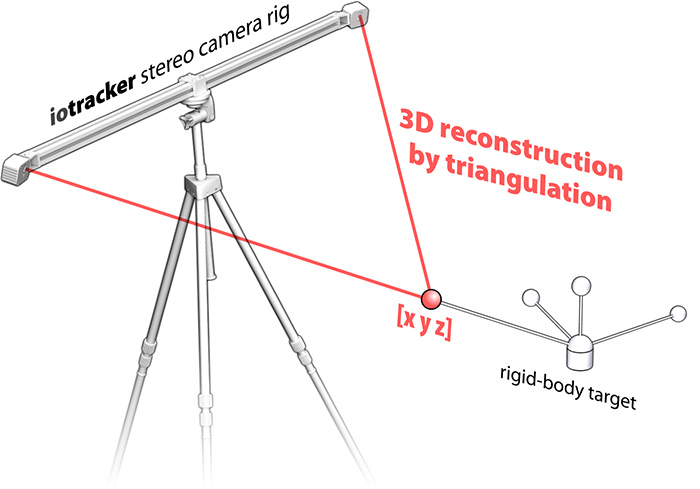
\includegraphics[scale=0.6]{figures/stereoCameras}
\caption{IOTracker optical triangulation demonstration}
\label{fig:stereo_cameras}
\end{figure}


\subsection{Methods for monitoring surroundings}
\paragraph{} As we could not find any information regarding to a fully automatic bicycle system, we decided to do research on fully automatic automobiles and take inspiration from that. After reviewing a few research papers, we came to the conclusion that our system needed to undergo 3 steps to monitor nearby obstacles (as mentioned by Weiming Hu \textit{et al.}  \cite{prediction_3D_vehicle_tracking}): motion detection, vehicle tracking and activity understanding.

\subsubsection{Collision Warning Systems (CWS)}
\paragraph{}CWS are usually incorporated into large vehicles such as transit buses because they are very prone to accidents due to it being more difficult for the driver to detect possible collisions with a more limited view of the vehicles surroundings. Although transit buses are a much greater size than bicycles, the idea of a CWS still remains. Mertz, C. \textit{et al.} \cite{CWS_transit_buses} describe the primary functions of a CWS as:
\begin{itemize}
\item Detect objects on the road under the tires
\item 360-degree coverage
\item Side and rear coverage for lane change manoeuvres 
\item High resolution
\item Distinguish between different objects
\item Spot rapidly approaching vehicles at longer distances
\item Estimate velocity of objects
\item Sensor system must not be too expensive
\item Few sensors
\item Reliable and easy to use and maintain
\end{itemize}

Mertz, C. \textit{et al.} \cite{CWS_transit_buses} also mention how a user interface should work in a CWS. Main features of an interface should include :

\begin{itemize}
\item Situation awareness: The situation around the user is displayed to the user
\item Alert: Non-intrusive indication informing the user of a potential collision
\item Warning: Intrusive indication informing the user of a dangerous collision is about to happen
\item Notification: Intrusive indication that a collision has occurred
\item Recording: Sensor data has been recorded for later analysis
\end{itemize}

\paragraph{}Most of these stages of interaction however should not apply to our system. For instance it would be obvious to the user if a collision has occurred; the situation surround the user would be much more visible on a bicycle; the system should prevent collisions from ever happening in the first place so a warning is not needed and sensor data would not need to be analysed for later review. In our case only an alert is much more appropriate as the user will only need to be informed of potential collisions and the system should take care of the rest automatically.

\paragraph{}Another interesting idea proposed by Mertz, C. \textit{et al.} \cite{CWS_transit_buses} is the use of cameras in stereo to obtain 3D information. This would mean that is possible to obtain information on the distance of objects using only cameras.

\paragraph{}There are a few concepts here that would work great for our system. However, a requirement of our system is to avoid collisions, not just warn the cyclist about them. Methods here should help provide a method of detecting objects to incorporate into further analysis so that the system can avoid collisions. 

\subsubsection{Vehicle Tracking}
{Weiming Hu \textit{et al.} \cite{prediction_3D_vehicle_tracking} suggest that there are 4 main categories of vehicle tracking:
\begin{itemize}
\item \textbf{Region-Based Tracking:} These are dependent on the variation of the image region in regards to the moving object. The background image is maintained and the motion is detected by removing the background from the current image. The algorithms only seem to work well on highways with little traffic as they cannot handle multiple vehicles in one image. 3D images of vehicles also cannot be acquired to get an approximation of the pose and orientation. 
\item \textbf{Active Contour-Based Tracking:} These represent the outlines of moving objects as contours. These provide more efficient descriptions of moving objects in comparison to region-based tracking algorithms. However, tracking more than one vehicle is still a problem. Also recovering a 3D pose of a moving object is a demanding problem. 
\item \textbf{Feature-Based Tracking:} These recognise and track objects by extracting elements, forming higher level features with them and matching the features between images. These adapt very quickly and successfully to allow real-time processing of multiple moving objects. However, the rate of recognition of vehicles is low due to distortion from perspective projection and movement relative to the camera. Also they cannot recover 3D poses nor handle tracking of multiple vehicles.
\item \textbf{Model-Based Tracking:} These track vehicles by matching a projected model over the image data. 3D wireframe models have been adopted in these algorithms.
\end{itemize}

\paragraph{}These methods of vehicle tracking all mention the use of 3D images. There are a few advantages of using 3D modelling, such as:
\begin{itemize}
\item Prior knowledge of 3D surfaces of vehicles provides robust tracking even when images include multiple vehicles.
\item 3D poses of vehicles can be obtained using camera calibration to set up geometric correspondence between 2D image coordinates and 3D world coordinates. 
\item Algorithms can be applied to take into account vehicles greatly changing their orientation.
\item 3D models can be generated offline.
\end{itemize}
\paragraph{}However there are also disadvantages of using 3D models as well. The main disadvantage being how computationally expensive it is. There are methods of reducing the complexity of using 3D models, such as the use of parametric models \citep{kollnig19973d}, but will still require more resources than when working in 2D.

\paragraph{Using a camera}As mentioned in Object Tracking: A Survey \citep{object_tracking_a_survey}, there is a strong relationship between object representation and the tracking algorithms. There are various ways of representing objects from a camera such as contour representation (described above), representation using points or skeletal models. Representation using primitive geometric shapes seems like a more suitable choice for our system because it seems needless to track detailed contours if we are trying to avoid objects of varying sizes and we are trying to conserve resources in the system. Also I believe vehicles can be easily modelled using geometric shapes. However this paper only considers 2D representations and not the use of 3D models. Selecting the right features of an image is important in tracking. Many features can be tracked, such as colour, texture and edges. For our case, it makes more sense to detect edges as the edges of an object are what determines a collision; but detecting colours may be useful for detecting lights on vehicles, which will help when tracking vehicles in the dark. 

\paragraph{Range Image Sequence} Range images are obtained using using a single-line laser range finder \citep{qualitative_car_tracking}. Car detection is based on prior knowledge of shape, size of vehicles and the assumption of the data being recorded off the ground plane. Vehicles consist of one to two line segments. Straight lines are detected using the Hough Transform (available in a c++ library \cite{cpp_houghTransform}).

\section{On board Computer}
\label{sec:computer}

\paragraph{}We initially researched a sole microcontroller that could be used for whole system functionality, as they are vastly used today in automatically controlled products (e.g. vehicle engine control systems), they offer onboard RAM and therefore do not need the configuration of separate components, reducing the risk of complications.  After research into the image processing algorithms we would be use for our detection and tracking of vehicles is was determined that a micro controller would not be sufficient to process the data, under detection and tracking algorithms, in real time. Processing in real time is crucial for this safety critical application and would become redundant if it did not. A quicker, multiple core, CPU was needed, that could offer parallel processing, which is essential as the application has to detect and track vehicle simultaneously from multiple cameras, among other tasks. The size of the RAM in micro controller also posed possible complications, given the amount of data that needed to be stored from each frame that was received from the multiple cameras. A computer board was decided upon, rather than obtaining separate components, such as CPU, motherboard, memory, etc. as were many reliable boards available, that have been widely used and tested for various application. The table \ref{table:board_comp} show a comparison between the various boards.


\landscape

\begin{table}[h]
\center
    \begin{tabular}{ | m{3cm} | m{2cm} | m{3cm} | m{3cm} | m{3.5cm} | m{1cm} |}
    \hline

    \center{\textbf{Computer Board}} & \center{\textbf{\# CPU Cores}} & \textbf{CPU core clock speed} & \textbf{RAM} & textbf{Wireless Connectivity} & \textbf{Cost}\\ \hline

 	  MinnowBoard MAX & 2 & 1.33 GHz & 2GB DDR3 & USB & �90.34\\ \hline
	RASPBERRY PI 1 MODEL 1 &  1 & 700MHz & 512MB & USB & �17.52\\ \hline
          Pandaboard & 2 & 1GHz & 1GB DRR2 & 802.11 b/g/n and Bluetooth 2.1 + EDR & 113.09 \\ \hline
         Jetson TK1 & 4 & 2.5GHz & 2GB & Additional PCIe board or USB&  �124.78\\ \hline
         Odroid-XUS & \pbox{20cm}{1. 4 \\2. 4} & \pbox{20cm}{1.2GHz \\2. 1,6GHz} & 2GB DDR3 & USB & 116.34 \\ \hline 
         MicroZed & 2 & 667MHz & 1GB DDR3 & USB & �129.33 \\ \hline

    \end{tabular}

\caption[Table caption text]{Wireless communication methods comparison} 
\label{table:board_comp}
\end{table}

\endlandscape

The Jetson TK1 computer board was chosen, as it ha been explicitly designed for vision based computation. 

\paragraph{}Microcontrollers are still necessary as they be used in the system to be able to connect to the CPUs digital Input and output, much like a keyboard connects to a standard computer, where a micro controller embedded in the keyboard is first used to determine which key was pressed by the user. These micro-controllers are used to connect the electrical components 

\section{Bicycle Brakes}

\paragraph{}Our system was primarily based around automatically stopping the bicycle when a collision was predicted, and a core component of that was the brakes. The brakes had to quickly and reliably halt the bicycle with a minimal stopping distance. We researched what had an affect on the latter and how it could be reduced. The stopping distance of a bicycle is calculated similarly to a vehicle (from when its brakes are fully applied), with the following considerable factors; tyre pressure, tyre diameter, tyre tread type, bicycle weight, cyclist weight, the coefficient of friction between the surface, current speed, driver reaction time and vehicle reaction time. Our system takes the reaction time of the cyclist away from the equation, as it should apply the bicycle brakes before the cyclist would have a chance to react. 

\subsection{Brake Lever}
\label{sec:brake_lever}

\paragraph{}The bicycle brakes had to have the ability to be activated via the bicycles on board computer and manually, via the cyclist, like a standard bicycle would. Different types of bicycle brakes were researched, for the aforementioned feasibility, but also that would provide the shortest braking distance. Common bicycle brakes use a bowman cable, hydraulic hose, or rods which are attached to the brake lever on one end and to the brakes on the other. The bowman and rods use the pressing of a level to pull the cables and, in doing so, pressing brake pads against a wheel rim or disc. The hydraulic hose, works like a vehicle hydraulic brake, where the lever being pressed forcing fluid towards the braking system causing a build up of pressure and causes the brakes pads to be pressed. 


%explain that "research" lead to the wanting to keep the standard of brake lever design and feeling that bicycle users were use to.

\paragraph{}We initially looked at a way of connecting these wire/hydraulic cables to, alongside the standard brake lever, to an electrical device, such as a motor (connected to the computer), which had the ability to increase and decrease the cable tension/pressure. We decided disregard this solution (explained in more detail in section \ref{sec:braking_component}, on page \pageref{sec:braking_component}) and decided that the users manual braking levers should be connected to the the onboard computer, via an electrical component, and would be activated with the same components as when automatically activated. This provided additional functionality, such as more control over the brakes and the force distribution to the front and back tyres; offers the user the ability to control how sensitive the brakes are (only for manual use), which is something that involves time consuming altering of mechanical components on a standard bicycle, but in this case the cyclist could easily alter the sensitivity to suit different riding conditions. Figures \ref{fig:early_brake_level_pressure} and \ref{fig:early_brake_level_pressure_enlarged} (page \pageref{app:early_sketches}), show sketches of where the component would be placed and how it would determine how much the brake levels have been compressed; the latter figure showing an enlarged and more detailed perspective.  

\begin{figure}[!htb]]
\centering
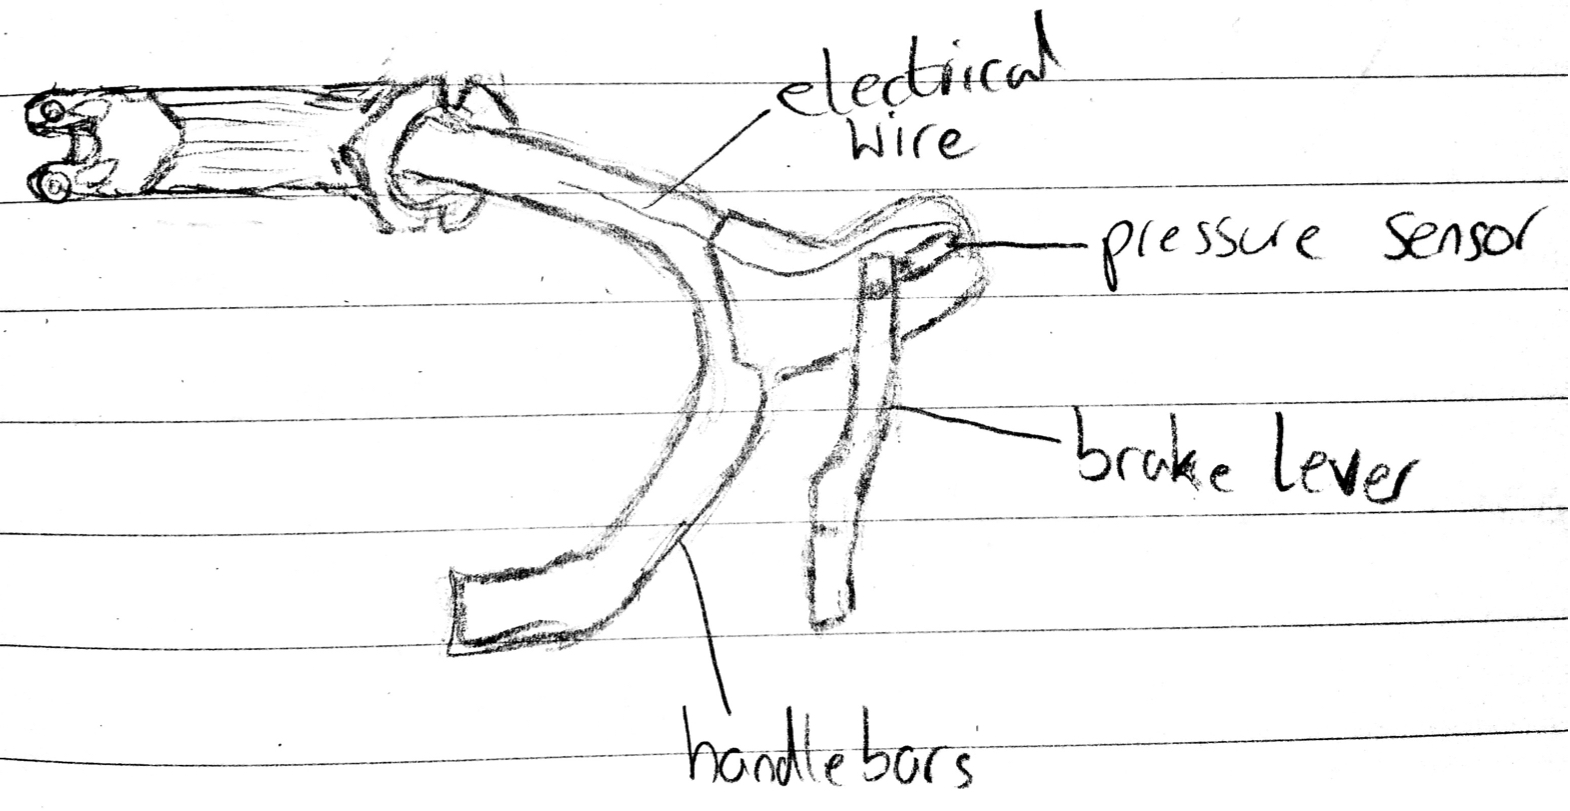
\includegraphics[scale=0.25]{figures/early_sketches/braking_system/brake_lever_pressure_switch}
\caption{Early design sketch of brake level attached to a pressure sensor for electrical braking system}
\label{fig:early_brake_level_pressure}
\end{figure}

\begin{figure}[!htb]]
\centering
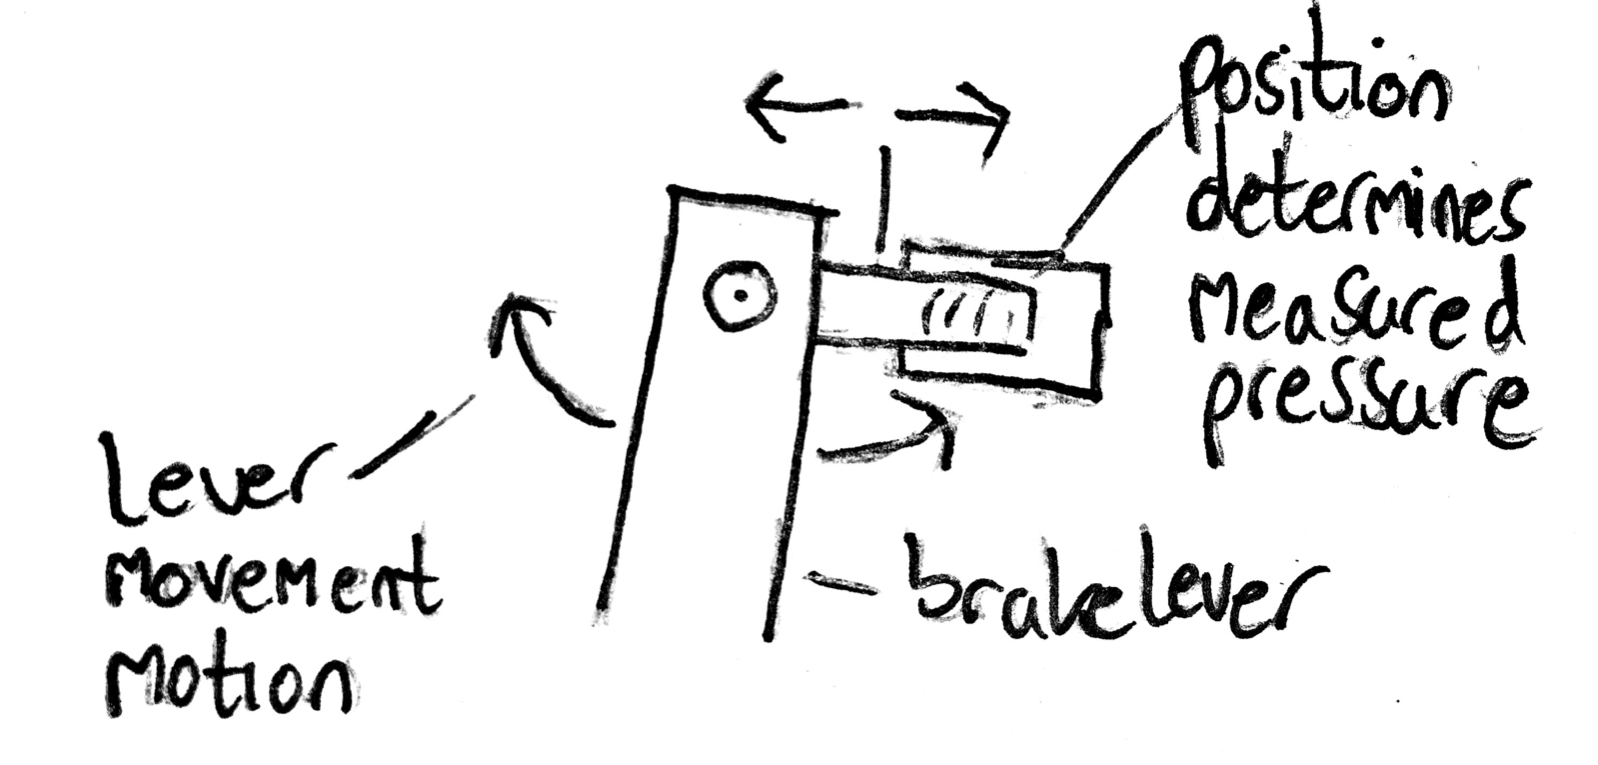
\includegraphics[scale=0.25]{figures/early_sketches/braking_system/brake_lever_pressure_sensor_enlarged}
\caption{Early design sketch of brake lever and pressure sensor enlarged from figure \ref{fig:early_brake_level_pressure} for electrical braking system}
\label{fig:early_brake_level_pressure_enlarged}
\end{figure}


\paragraph{}We researched the type of sensor that we could use for converting the force applied via the compression of the lever and discovered a component called a 'Load Cell' or by some manufacturers, a 'Force Transducer' (see fig \ref{}  on \pageref{}) which outputs an electrical signal proportional to the amount of force applied. After analysis of our early design and the load cell components design, we came to the conclusion that the component was not suitable for our application, as it appeared that the component was used in applications for industrial measurements; we also realised that the internal design of the brake levers would require an attached spring, so the lever would decompress once released, like on a standard bicycle (whereby the lever decompresses via the released hold on the wire). This lead to the research into spring based sensors (e.g. a spring based resistor/potentiometer). 

\paragraph{}A spring potentiometer was discovered to be used in many applications; the two most significant applications being for a vehicle foot pedal, and even more so, for twist throttles on a motorcycle. Figure \ref{fig:spring_pot} (appendix section \ref{app:brakes_current_technology}, page \pageref{fig:spring_pot}) illustrates the design of such a component. It has a rotary subcomponent which is attached to a spring and rotating this subcomponent clockwise causes a change in resistance, which affects the electrical output. This electrical output can be used to determine how much the lever has been pressed and therefore how much to apply the brakes. An important factor of this component, is that it can be self returning (via the spring), offering similar functionality to what people have come accustomed to on a standard bicycle brake levers.

%one more sketch showing the internal use of the chosen spring potentiometer 

\subsection{Braking Component}
\label{sec:braking_component}

As briefly mentioned in section \ref{sec:brake_lever}, was to offer the standard manual braking alongside the automatic braking, and figure \ref{fig:early_motor_cable_tension} (appendix \ref{app:early_sketches}, on page \pageref{fig:early_motor_cable_tension}) shows a simplistic early sketch of how this may have operated for one brake. This implies there would be two electrical motors attached to the brake cable. This was short-lived solution, as an issue with this solution was that, given the front and back brakes are at different distances from the handle bar brake levers, different tension/pressure is needed, and therefore two separate motors for pulling and release the cables would have been needed, for each brake. There are multiple problems with having two motors; it would be difficult to maintain an equal distribution to the front and back brakes and if a non equal distribution occurred, then safety issues arise. More devices also increases the number of components where a fault could occur and thereby risks increasing the amount of maintenance.  

\paragraph{}In keeping with the electrical components we had decided to use in the brake lever, and the above flaws of using an electrical component, such as a motor, combined with the standard functionality of a bicycle, we decided that the braking component should also be electrically activated, but in this case it could be an electrical motor attached directly to the brake and used rotary motion to apply or release the brakes directly. This type of device, in conjunction with section \ref{sec:brake_lever} concluded component, offers a fast response, precise control of the brakes, and the ability to include known braking technology to increase control and reduce skidding.

We researched into current electrical braking, in bicycle and vehicles. There was near to nil examples for electric brakes on bicycles as it's not a technology that has been required, but we did discover a professor \cite{wireless_bicycle_brakes} who had developed a wireless braking system (see figure \ref{fig:wireless_bicycle_brakes}, appendix \ref{app:brakes_current_technology}, on page \pageref{fig:wireless_bicycle_brakes}), that used an electric motor to activate the disc brake. We also drew inspiration from the vehicle manufacturer Audi and their Electric Hydraulic Combe brakes (EHCB) (see figures \ref{fig:audi_EHCB_1} and \ref{fig:audi_EHCB_2} in appendix section \ref{app:brakes_current_technology} page \pageref{app:brakes_current_technology}). See section \ref{sec:comp_design_brakes} for the braking system component.

%need to calculate stopping distance :/ 

\subsection{Communication}
\paragraph{}We had to decide how the subsystems of the product would communicate with each other. The electrical brake lever and braking components could have been adapted to be wireless, but there was no application for such measures and it would have added further complexity, reduce transmission speeds and posed a risk of disconnection, which was not acceptable given the time criticalness of the application. These components are connected to the computer board and micro controllers via standard electrical wiring, which is hidden within the inside of the bicycle frame. A decision whether core components such as the vision cameras and smart phones would connect to the computer board was more considered decision, whereby the advantages and disadvantages of both methods were considered. A devices were also considered and practicality of different methods.The most imported specifications of popular wireless and wired communications were collected and collated into a table \ref{table:wireless_comp} and \ref{table:wired_comp}, respectively.

\subsubsection{Cameras}
The vision cameras were primarily designed to be used via a usb interface and thereby they performed at their optimal capabilities when using this method. This was an ideal solution though, as cameras are a fixed component, that the user does not have to adjust or interfere with and therefore a wired usb connection through the inside of the bicycle frame could be used. 

\subsubsection{SmartPhone}We concluded that the smartphone should connected to the on board computer via Bluetooth 4.0. The first reason for this decision was that smartphone have varying manufacturers and therefore have a number of different wired connection methods, which we would have had to have accommodated for by the user having to connect their smartphone into a USB port (The USB on the device is solely so the user can charge their device.). Secondly, with the use of a wireless method we had the option to incorporate other features, such as remote locking of the bicycle. The decision of bluetooth 4.0 was its known capabilities of operating under low power; a crucial necessity for our application which was dependent on a battery power supply. A method know as WiFi Direct (or Wi-Fi P2P) which is a peer-to-peer wifi connection that does not require a physical wireless access point, such as a router; instead one device will be determined to act as the access point during pairing, meaning that only one of the two devices has to be equipped with Wi-Fi Direct.  This required more power to operate and it wasn't as integrated into smart devices as Bluetooth and was therefore dismissed. NFC was disregarded for its immediate limitation with its maximum range, as is was not suitable for a device that may be required to communicate with other devices, given that the average length of a bicycle is 178cm and therefore limits the positioning of those devices on a bicycle. 

\subsubsection{On-board computer}With the decision that the connection the smartphone would be via Bluetooth 4.0, this was obviously an essential component that needed to be attached to the Jetson TK1 computer board, to enable communication with the smartphone, for displaying sensor information and for radius remote locking. The computer had to be able to access the internet to interface with the database, for details regarding the specific user and multiple wireless methods were considered. 

\paragraph{Internet Access via tethering} A device such as an embedded computer with bluetooth or Wi-Fi modules could connect to another device that also has either of these modules (or via physical connection), plus the compatibility to connect to the internet, and use a technology known as ?tethering? to share internet access. This would reduce overall costs of a device, but would require an external device to gain internet access.

Wi-Fi access point is usually the best type of access to the internet, providing faster and more stable data transfer than 4G. Unfortunately it is still a technology that is designed to be used within a radius of a central point (access point) and is therefore not feasible for connected devices on a moving bicycle to a central database, etc.  

Future use?.  handover

3G

This is the third generation of mobile technology and is still in great use today. It is the standard that networks providing 3G must ensure a data transfer of more than 200 Kbit/s, though most cell towers will provide speeds 

\begin{landscape}

\begin{table}[h]

   \center
    \begin{tabular}{ | m{3cm} | m{3cm} | m{3.5cm} | m{3cm} | m{3cm} | m{2.5cm} |}
    \hline
    \textbf{Wireless comms} & \textbf{Max Data Rate} & \textbf{Security Protocol} & \textbf{Encryption} & \textbf{Range} & \textbf{Backwards Compatible}\\ \hline
   
   Bluetooth v2.0 + EDR & 2.1 Mbit/s & Pairing Authentication Protocol & 128 bit stream cipher & \pbox{20cm}{Class 3 radiios: 1m \\Class 2 radios: 10m \\class 1 radios: 100m} & v1.2  \\ \hline
   Bluetooth v2.1 + EDR & 3 Mbit/s & Pairing Authentication Protocol & 128 bit stream cipher & \pbox{20cm}{Class 3 radiios: 1m \\Class 2 radios: 10m \\class 1 radios: 100m} & v2.0 \\ \hline
   Bluetooth v3.0 HS & 24 Mbit/s & Pairing Authentication Protocol & 128 bit stream cipher & \pbox{20cm}{Class 3 radiios: 1m \\Class 2 radios: 10m \\class 1 radios: 100m} &  v2.1 and v2.0\\ \hline
   Bluetooth v4.0 + EDR & 3 Mbit/s &Pairing Authentication Protocol & 128-bit AES with Counter Mode CBC-MAC & \pbox{20cm}{Class 3 radiios: 1m \\Class 2 radios: 10m \\class 1 radios: 100m} & v3.0, v2.1 and v2.0 \\ \hline
   Neat Field Communication (NFC) & 424 Kbit/s & N/A & \pbox{20cm}{AES \\(not required by \\standard)} & < 20cm & N/A \\ \hline
   Wi-fi 802.11b & 11 Mbit/s & WPAv2 & AES 256 bit & 250 m & 802.11a\\ \hline
   Wi-fi 802.11g & 54 Mbit/s & WPAv2 & AES 256 bit & 250m & 802.11b \\ \hline
   Wi-fi 802.11n & \pbox{20cm}{600 Mbit/s \\(theoretical)} & WPAv2 & AES 256 bit & 250m & \pbox{20cm}{802.11a  \\802.11b \\802.11g} \\ \hline
   Wi-fi 802.11ac &  \pbox{20cm}{1.3 Gbit/s \\(theoretical)} & WPAv2 & AES 256 bit  & 250m & \pbox{20cm}{802.11g \\802.11n} \\ \hline
   Mobile 3G & 3 Mbit/s & \pbox{20cm}{UEA1 \\UIA1} & KASUMI & 5 - 22 miles [2] & 2G \\ \hline
   LTE 4G & \pbox{20cm}{3 - 10 Mbit/s \\(theoretical 100 \\Mbit/s)} & \pbox{20cm}{UEA1 \\UIA1} & SNOW 3G & 5 - 22miles [2] & \pbox{20cm}{2G \\3G}  \\ \hline
   
    \end{tabular}

\caption[Table caption text]{Wireless communication methods comparison} 
\label{table:wireless_comp}
\end{table}

\end{landscape}

\begin{table}[h]
\center

    \begin{tabular}{ | m{2.5cm} | m{2.5cm} | m{3.5cm} | }
    \hline
    \textbf{Wired comms} & \textbf{Data Rates} & \textbf{Max Cable Length (without repeater) } \\ \hline
  
  Ethernet Cat 5  & 10/100 Mbit/s & 100m\\ \hline 
  Ethernet Cat 5e & 10/100/1000 Mbit/s & 100m\\ \hline
  Ethernet Cat 6 & 10/100/1000 Mbit/s and 10 Gbit/s & \pbox{20cm}{100m @ 1000Mbit/s \\55m @ Gbit/s} \\ \hline
   USB 2.0 & \pbox{20cm}{450 Mbit/s \\(theoretical)} & 5m \\ \hline
   USB 3.0 & \pbox{20cm}{5 Gbit/s \\(theoretical)} & 3m\\ \hline
   USB 3.1 & \pbox{20cm}{10 Gbit/s \\(theoretical)} & 3m\\ \hline
    \end{tabular}

\caption[Table caption text]{Wired communication methods comparison} 
\label{table:wired_comp}
\end{table}

\chapter{System Architecture}

\section{Architectural Design}
\paragraph{}The design of the architecture went through several iterations. Our initial design was to have wearable technology (as well as a mobile phone) link with the bicycle, with the wearable technology displaying the interface to the user while all complex computation is to be done in the bicycle. A component diagram was developed to show how the software components link together with the hardware components to make the overall system (see figure \ref{fig:component_arch}). However the idea of using wearable technology was scrapped and we decided on only using a mobile phone as an interface. 

\begin{figure}[h]
\centering
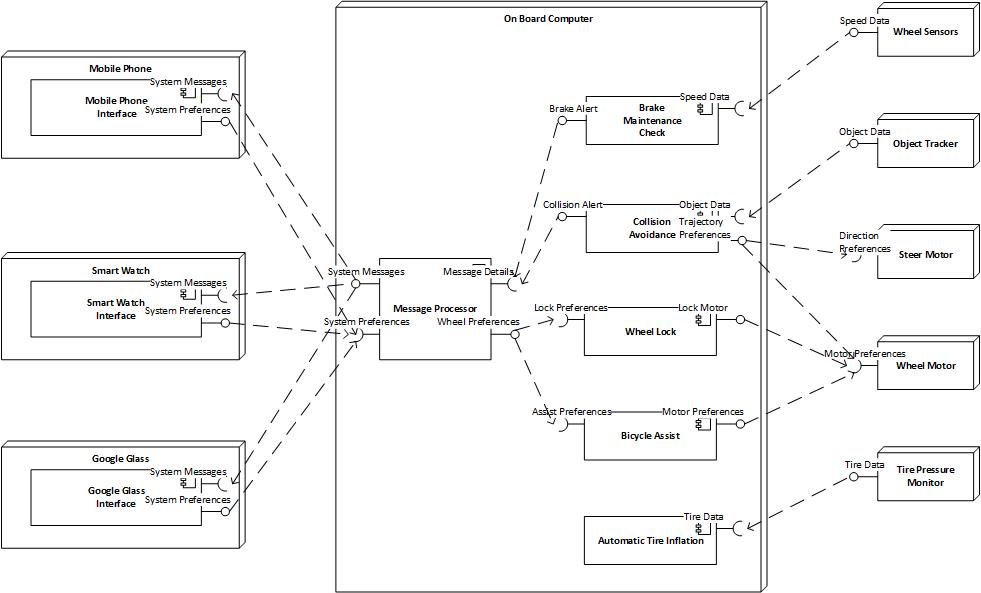
\includegraphics[scale=0.6]{figures/system_architecture/component_arch}
\caption{Component diagram of initial architecture}
\label{fig:component_arch}
\end{figure}

\paragraph{}The UML class diagram shown in figure \ref{fig:UML_Class_Diagram} displays the final structure for the software components of the system and figure \ref{fig:overall_sys_arch} shows how we expect the final system to be deployed. We included the use of an online database as we gave the option for the user to save their preferred settings and back them up online via an account system. 

\begin{figure}[h]
\centering
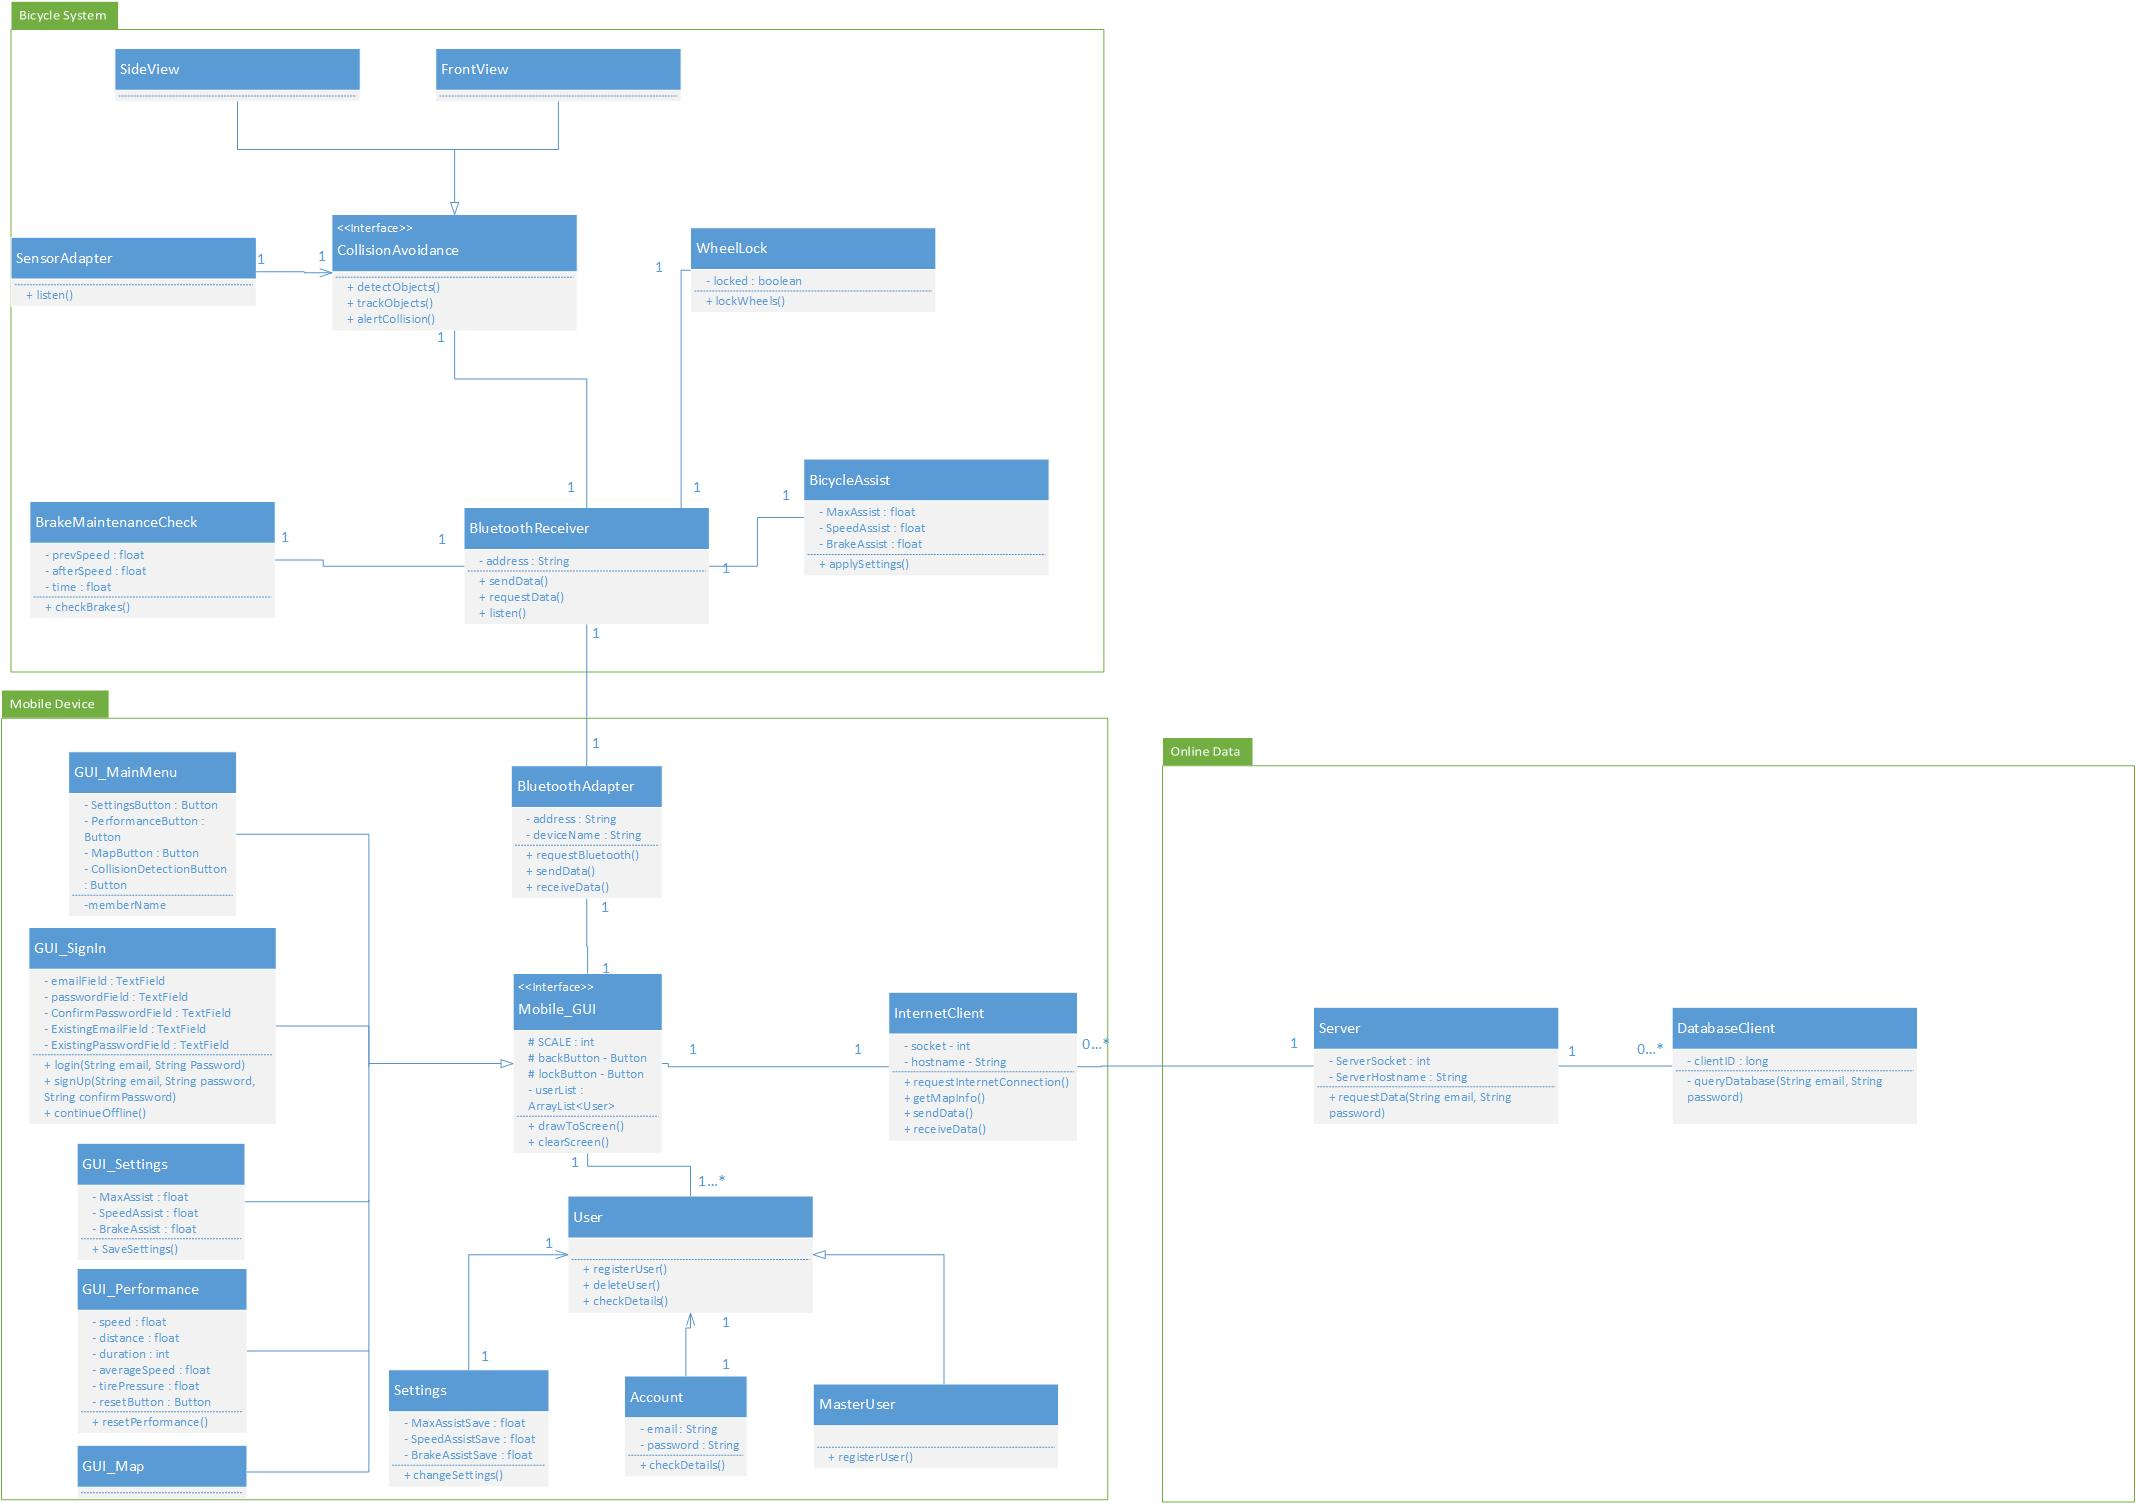
\includegraphics[scale=0.4, angle=90]{figures/system_architecture/UML_Class_Diagram}
\caption{UML Class diagram}
\label{fig:UML_Class_Diagram}
\end{figure}

\begin{figure}[h]
\centering
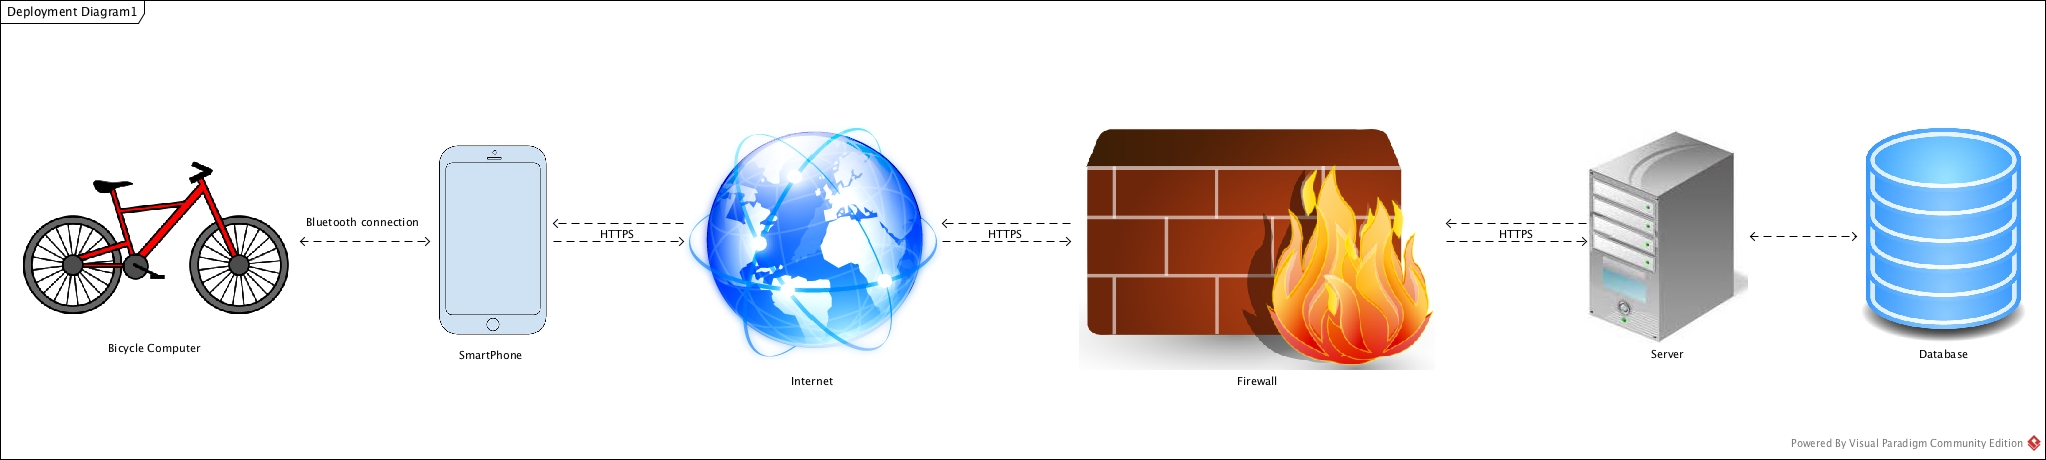
\includegraphics[scale=0.2]{figures/system_architecture/overall_sys_arch}
\caption{Deployment of the overall system architecture}
\label{fig:overall_sys_arch}
\end{figure}

\chapter{Data Design}
\section{Data Description}
This system is not heavily data driven and for a long time during the design there was to be no backend database at all. Once we had decided against the crowdsourced route planning idea (section \ref{subsec:rejected}) we felt that there was no need to have data stored in a backend database/cloud and that it would create more problems than it would solve (security, accessibility, etc.). However when we began to design the user interface we started to look at this from a more user centred position and saw the obvious benefits to having data stored remotely.
\subsection{Bicycle Settings}
From a very early stage we decided that in order to make the user experience as good as possible the user should be able to easily customise the settings of the bike. Ideally we want every single aspect of the bike to be customisable - that may not be possible due to limitations of the hardware or software available, but that was our overall aim. 

Under our initial plan we wanted to keep things as simple as possible and went with a purely sensor based approach where the current readings can be read by the computer in order to tell the user the current state of the bike and the user would update the settings and whatever it is that is being changed would change. Here the values would not be saved, they would just be read from the sensors every time. This is very easy and cheap to implement but it turns out it is not really very suitable, for the following reasons:
\begin{itemize}
  \item This works very well for purely mechanical settings, such as suspension firmness or ride height, however we would also like some more adaptive settings, such as brake assist level and maximum motor speed. These settings are hard to adjust mechanically and would probably require some computer control.
  \item This is very sensitive to the accuracy of the sensors, if one of the sensors starts to give faulty readings it will be very difficult to recover the behaviour that you had set up.
  \item It is practically impossible to recover settings. If the bike were to suffer a major error there is no way to save settings or move them to a new bike.
\end{itemize}
From here we moved to a system where the settings are stored locally on the bike and will then be changed via the interface and updated on the bikes local memory. Then, whenever the user gets on the bike they would not need to play with settings as they would already be loaded. This addresses many of the problems mentioned above but is not perfect.
\begin{itemize}
  \item Although users will now quite easily be able to save a backup of their settings and transfer them to a new bike - they will not be able to recover settings on the go and the system will not really be practical for somebody who uses multiples bikes (somebody who lives a two addresses, for example).
  \item Equally, this system would need to be adapted to allow for multiple users on the same bike.
\end{itemize}
This is what led us to our final cloud based approach. We first approached this by saying that the settings are a property of the bike, that multiple users can modify. However, after talking to our user group we found that it would clearly be more appropriate for the settings to be attributed to the users themselves. This would be particularly beneficial for users who have multiple bikes but also resolves a potential annoyance whereby a user may have had to change the bike settings every time they go to use it (if somebody has used the bike in the meantime). The drawback to this approach is that it does not allow for one user to have different settings for each of their bikes, since the settings are not attributed to the bikes but rather the users. However, the users that we spoke to said that this way would be more beneficial to them.


\subsection{User Access}
In order to properly implement the bike settings we would need each user to have their own unique login so that the could associate settings with that account. This actually became quite a major issue for us because we had the following requirements:

\begin{itemize}
\item A user should be able to access multiple bikes, if they so wish
\item Multiple users should be able to access one bike
\item A user should be able to have their personal settings download automatically on any bike that they use
\item A user should be able to access their bikes with relative ease
\item User access should be restricted to certain people
\end{itemize}

\subsubsection{Security}
The key issue that we had to solve was how to pair users with bicycles in such a way that it is easy to do but also doesn't allow any random person to pair themselves. After considering many solutions; such as allowing anybody to pair, but restricting who can lock and unlock the bike to just one person. This wasn't practical because it meant you wouldn't be able to cycle somewhere and lock the bike without the locking users credentials, which then compromises the integrity of the system. Another approach that was considered was assigning accounts to the bikes rather than the users - but this would not be very good either because then users would need to remember account details to log into different bikes - and it also makes the settings more difficult to implement.

The final solution that we eventually came up with was almost a combination of both ideas - we had to make a slight trade-off towards security over ease of use in this situation. We decided on a system of master accounts. Where on the initial setup of the bike a master account is assigned and then this master account holder is then able add or remove other users to the bike. This is not ideal for users who jointly own a bike where there is no obvious master account holder and it is also not ideal for a bike that is used by lots of different people because it could require the master account holder to be making regular changes. However we felt that these situations are rare, workable and also that the security implications make this necessary trade-off. 

\subsection{Future applications}
Many modern applications now make use of the huge amount of information available online by networking with other applications such as Google+ and Facebook. This is true of many of the cycling applications that we looked at which allow users to do things like share their routes with friends, view cycling statistics about each other and some even introduce some friendly competition. Although this is not an element of our design it something to keep in mind for the future - and by storing user accounts in a cloud server it is much easier to associate each account with a Facebook or Google+ account at a later date.

\section{Communications}
All internet traffic between the bicycle and the user will go through the HTTPS protocol, which uses the Transport Layer Security (TLS) protocol to offer encrypted data. TLS Uses X.509 certificates (Public Key Certificate standard), which uses asymmetric cryptography, to ensure the authenticity of party and to exchange a symmetric key. The authenticity of our domain w This symmetric key can be used for the rest of the session or after a time interval. The use of X.509 certificate will require the use of  certificate authorities, as people can most people will not be able to trust the authenticity of a self signed certificate.

As well as this all user passwords should be stored using a secure hashing algorithm, this means that the plaintext passwords are not saved anywhere and if the database was compromised the user passwords would still be protected. As a further level of protection passwords should be salted to prevent against dictionary attacks on the password hashes.
\section{Database Schema}
\begin{figure}[h]
\centering
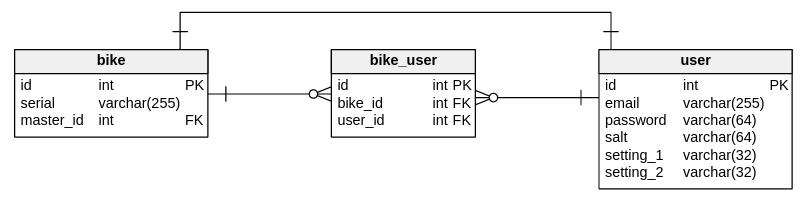
\includegraphics[scale=0.5]{figures/sql}
\label{fig:sql_schema}
\caption{Basic SQL schema for the database}
\end{figure}

In figure \ref{fig:sql_schema} you can see the basic SQL schema required for this system. In order to achieve the many-to-many relationship required between bikes and users we had to incorporate a `bike\_user' table to link the two. As well as this we had to be able to identify the master user this could be done in a few different ways. We could have had a boolean field in the relationship table identifying whether this was a master relationship, along with this we would need a constraint to specify that there should be one and only one master flag set to true for each bike\_id. The approach we actually went for was to have the master\_id stored in the bike table directly. This removes the need to check that there is one and only one master and also makes it much easier to manage the situation where the master user `gives up' the bike. This will require it's own constraint; that the master user is already specified as a user of that bike in the bike\_user table.
\chapter{Component Solutions}
\label{sec:component_solutions}


\section{Braking System}
\label{sec:comp_design_brakes}

\paragraph{}In section \textbf{\ref{sec:brake_lever} \nameref{sec:brake_lever}}, it was concluded that a practical solution was to use a self returning rotary potentiometer, due to the advantage it provided. There was a decision whether the brake lever components would be directly connected to the main on board computer or whether they would be connected to a microcontroller, which would then be connected to the core computer board via a serial connection. The latter was decided upon, as it offered reduce complexity, greater flexibility and maintainability; and reduced processing overhead on the main computer, which could be processed on a separate microcontroller, whereby its sole purpose is for embedded solutions, offering better design for electrical components. In addition, given the choice of the main computer board, Jetson TKS (\textbf{\ref{sec:computer} \nameref{sec:computer}}), it is better practice as the application is using motors and a PWM (Pulse Width Modulation) is used to control the speed of such devices and having PWM directly on the Jetson TK1 then it might not provide stable signal timing \cite{jetson_microcontroller_support}. 

\subsection{Iteration I}

\paragraph{}All electrical components are connected to the micro controller, shown in figure \ref{fig:braking_schematic}. The Jetson TK1 is connected to the microcontroller, via a 2 way serial UART connection. The connection needs to be two way, as the as Jetson TK1 needs to receive data form the microcontroller, regarding the electrical components, and it needs to be able to transmit control data. The Jetson TK1 controls the operation of the motors, by processing calculations and then sending the control data to the micro controller, whereby it performs the PWM. The micro controller will also send the digital data regarding the brake lever components to the main computer board, after the analog signals have been converted to digital representation (via the ADC), shown in algorithm \ref{alg:brake_lever}. The main program on the Jetson board, alongside processing collision detection, will be controlling the brakes in response to the rotary potentiometer (brake lever) data received from the microcontroller. The program will then process varying decisions and transmit motor controls to the microcontroller. The data will be the brake that was operated and how much force was applied (represented by a digital voltage value) and that value determines the motor speed. 


\begin{figure}[h]
\centering
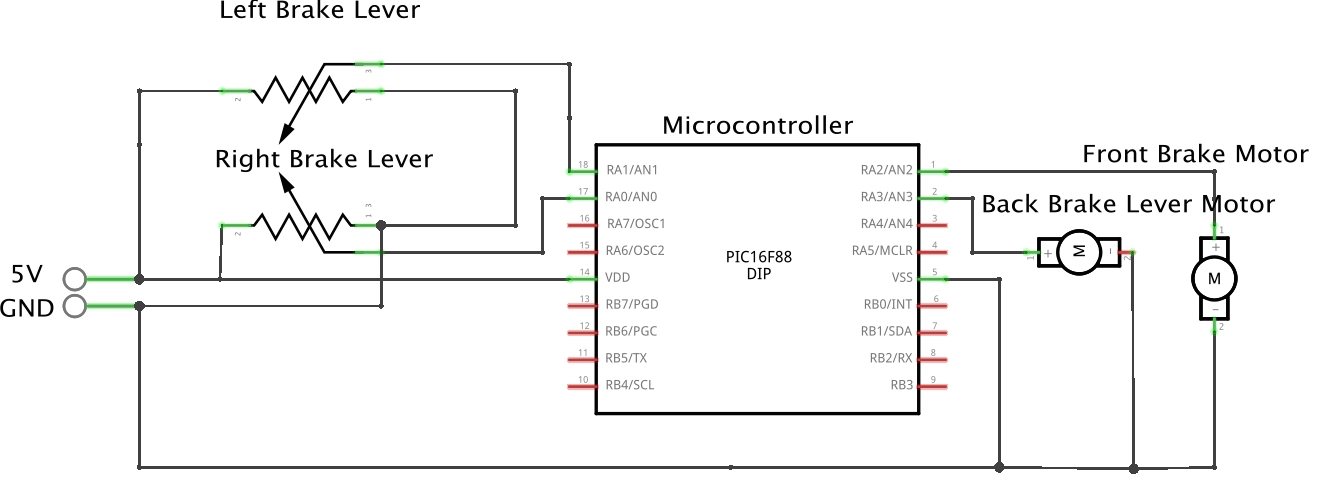
\includegraphics[scale=0.3]{figures/electronic_braking/circuit}
\caption{Electronic braking schematic (with omitted components; not necessary for core explanation)}
\label{fig:braking_schematic}
\end{figure}

\begin{algorithm}[h]
\caption{Manual Brakes Applied}\label{lag:brake}
\begin{algorithmic}[1]
\State $brakeLever := PressedLever$\Comment{The left or right brake lever}
\State $brakeVoltage := \Call{AnalogVoltToDigital}{voltage}$\Comment{analog volt value to digital representation}
\State $brakeAngle := \Call{CalculateBrakeAngle}{brakeVoltage}$\Comment{calculating angle from voltage}
\State $\Call{ControlMotors}{brakeLever, brakeAngle}$\Comment{control motors based on brake lever and brake angle}
\end{algorithmic}
\end{algorithm}

\begin{algorithm}[h]
\caption{Analog to digital voltage conversion Lever}\label{alg:brake_lever}
\begin{algorithmic}[1]
\Function{AnalogVoltToDigital}{}
\State \Call{delay}{n}  \Comment{Delay for circuitry to receive analog signal e.g. 20$\mu$s} 
\State $ADCRegisterGOBit := 1$
\While{$ADCRegisterGOBit == $}\Comment{Wait for conversion to complete}
   \EndWhile\
   \State $adcResult := ADCResultRegister$\Comment{Get the result stored in the result register}
\State $return adcResult$
\EndFunction
\end{algorithmic}
\end{algorithm}

\begin{algorithm}[h]
\caption{Calculating brake lever angle from voltage}\label{alg:brake_angle}
\begin{algorithmic}[1]
\Function{CalculateBrakeAngle}{$voltage$}\Comment{digital voltage received from the microcontroller}
\State $brakeVoltage = voltage$\Comment{The voltage received from operating the electrical lever}
\State $MAXLEVERANGLE := 45$\Comment{Max angle the break lever can rotate the potentiometer}
\State $MINLEVERANGLE := 0$\Comment{Min angle the break lever can rotate the potentiometer}
\State $DEGREESPERVOLT := 0.72$\Comment{0.72\degree is 0.01 volts}
\State $VOLTPERDEGREE := 0.01$\Comment{0.01 volts to each 0.72\degree}
\State $brakeAngle := brakeVoltage / VOLTPERDEGREE * DEGREEPERVOLT$
\State $return brakeAngle$\Comment{return the calculated brake angle}
\EndFunction
\end{algorithmic}
\end{algorithm}

\begin{algorithm}[h]
\caption{Control Brake Motors}\label{alg:motor_control}
\begin{algorithmic}[1]
\Function{ControlMotors}{$brakeLever, brakeAngle$}

\If{$brakeLever == LEFTLEVER$}
	\State{$motor := BACKMOTOR$}
\Else
	\State{$motor := FRONTMOTOR$}
\EndIf

\If{$brakeAngle < \Call{CurrentAngle}{motor}$}
	\State{$\Call{rotateMotorCounterClockwise}{brakeAngle}$}
\Else
	\State{$\Call{rotateMotorClockwise}{brakeAngle}$}
\EndIf
\EndFunction
\end{algorithmic}
\end{algorithm}

\subsection{Iteration II}
Instead of the Jetson TK1 processing the decisions regrading the braking system when manually operated, it was decided that the embedded program on the microcontroller should decide upon the motor control based on the input. This was decided as having the Jetson TK1 process task that could be done on the microcontroller, used valuable resources. There is no more communication delay from the computer board and microcontroller. The 2-way serial UART connection remains, as the Jetson Tk1 still needs to provide motor control command to the microcontroller when an automatic braking occurs, which would override any braking by the user that could reduce the braking impact. Some of the algorithms on first iteration also didn't account for the user pressing the brakes simultaneously, or whether the currently running code would block until finalised. The \ref{alg:motor_control} would have to operate both motors simultaneously. The microcontroller does not have multiple cores and therefore has to used single core multiple threading software techniques. If both the brake levers have been operated then each part of the motor control for the front wheel and the brake wheel will be operated for small amounts of time. The amount of time each task will be given is also in proportion to angle at which he brake lever has been pressed, as that brake is a higher priority as the user wants it to apply more force to the disk brake.

\section{Collision Avoidance System}

\subsection{Interface Description} What does the components interact with (other software, hardware) diagram?

\subsection{Possible Solutions} Collision has to be broken down into 4 different steps (detection, tracking ...)

\subsubsection{Preceding Vehicle Trajectory Prediction by Multi-Cue Integration \citep{multi-cue}}

\paragraph {} This is paper \citep{multi-cue} detects and tracks preceding vehicles using a monochrome camera to predict whether the vehicle is going to change lane (in a left or right direction) or stay in its current lane. This involves the detection and tracking of both vehicles and the road lines they reside in. It uses Support Vector Machine (SVM) with a motion and appearance cue to recognise driver pattens, that are trained for a two class feature set. The two class features are used to predict lane-changing recognition, via the input of timestamped 3D positioning. 

\paragraph{}A kalman filter is used to track the motion of the lane boundary and predict from frame-frame its new location. There is an intersection between two lane boundaries, which is known as the vanishing, and is used to detect the pitch angle change of the camera. Line features are used to establish vehicle hypotheses, which are verified by an SVM (with HOG) trained for vehicle recognition via a pre-learned vehicle model database. Post verification, a Kanade-Lucas-Tomasi feature tracker is used and the bottom of the tracked vehicle in each frame to calculate its 3D position.
\paragraph{Advantages}
\begin{itemize}
\item Tested on real-world data via a vehicle on a highway
\item Lane changing warning is warned in real-time
\item The whole system achieves 10hz on a 1.8 GHz Dual-Core CPU
\end{itemize}

\paragraph{Disadvantages}
\begin{itemize}
\item The system requires lanes to infer whether a collision is probable	 	
\end{itemize}

\begin{figure}[h]
\centering
	\begin{minipage}{0.49\textwidth}
		\centering
		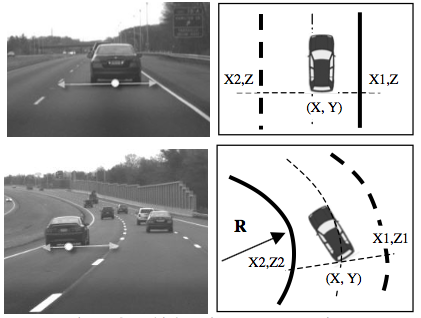
\includegraphics[scale=0.4]{figures/research_paper_figures/trajectory_multi-cue}
		\caption{Vehicle trajectory computation at straight and curved lanes \citep{multi-cue} }
		\label{fig:traj_multi-cue_image1}
	\end{minipage}\hfill
	\begin{minipage}{0.49\textwidth}
		\centering
		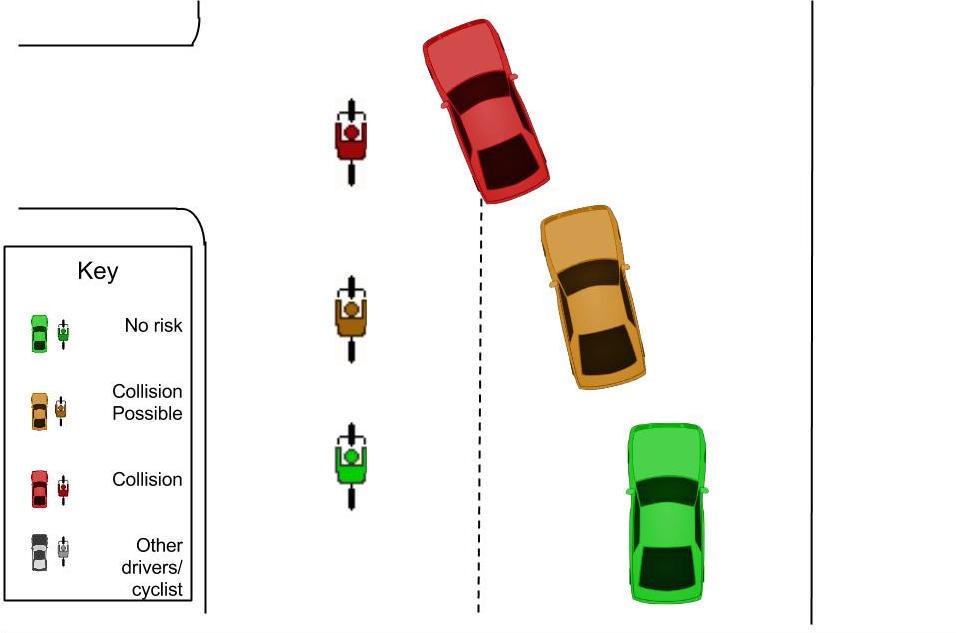
\includegraphics[scale=0.2]{figures/collision_avoidance_figures/Vehicle_changing_lane_into_the_path_of_a_cyclist}
		\caption{Cyclist and vehicle lane changing collision}
		\label{fig:change_lane_image}
	\end{minipage}
\end{figure}

Fig. ~\ref{fig:traj_multi-cue_image1} on page~\pageref{fig:traj_multi-cue_image1} shows the lane change tracking and prediction that this papers algorithms accomplish and Fig. ~\ref{fig:change_lane_image} on page~\pageref{fig:change_lane_image} shows, one of other, cyclist collisions that we want to prevent. This paper displays a high chance of solving this issue.


\subsubsection{Learning Multi-Lane Trajectories using Vehicle-Based Vision \citep{multi-lane_traj}}

Conclusion - decision complying with criteria at the start

\section{CPU}
The Central Processing Unit (CPU) is key to the whole system - it is the CPU that will be programmed to make the crucial decisions.
\subsection{Component Requirements}
In general the requirements for a CPU are fairly simple - computing power - and is often not a major consideration. However, given the mobile nature and safety critical elements of this design there are a few important things we had to keep in mind while choosing an appropriate CPU.

\begin{itemize}
  \item The CPU should be able to analyse potential collisions in (near) real-time
  \item The CPU should 
\end{itemize}
\subsection{Interface Design}
The CPU is the HUB of the whole system - it will be connected to every component of the system.

The CPU will be constantly reading the inputs from all of the sensors in the system, processing the data and then sending signals to the output systems; the braking system or the user interface for example. 
\subsection{Possible Solutions}
\paragraph{Conculsion}

%JACK brakes and why we decided to reject the automatic steering.


\chapter{Prototype Analysis}
\label{ch: prototype}
Prototyping is a very important part of the user-centred design process as this was the main opportunity for us to integrate user feedback into our design. This section will explain all of the major issues that we had to address because of our prototypes and the decisions we made as a result. There were two major components to our solution:
\begin{itemize}
  \item The bike hardware. Here we were trying to position all of the components (cameras, lights, battery, etc.) in the ideal position. We had to make sure that all of the components were positioned somewhere sensible and functional.
  \item The interface. These are the screens that the user directly interacts with to modify their settings and view statistics. The interface should allow the user to perform all of the key tasks with easy and efficiency.
\end{itemize}
We created some lo-fi prototypes for the interface using, the wireframing software, Balsamiq\cite{balsamiq}. This was particularly useful because it allowed us to create prototypes quickly and test them fairly easily. All of which helped us to receive, and then act on, user feedback. However it was not so easy for us to prototype the hardware due to our limited resources. We had to prototype the hardware using only sketches which was not ideal because it did not allow users to really get a feel for the design and how things interact. This meant we had to use our own knowledge of the product (and problem space) much more in this area.

\section{Prototype 1}
\label{sec:phones}
Analysis of the initial prototype sparked a discussion about the best medium for the interface. Initially we had decided to present the interface as a smartphone application, there were many reasons for this decision:
\begin{itemize}
  \item \textbf{Portability} The primary advantage of using a smartphone, from our point of view, was that it would allow users to change their settings on-the-go. We felt that this would be hugely beneficial for users if they can change their settings while they are away from the bike and have them automatically download whenever they start to ride. 
  \item \textbf{Cost} Having users simply download a free application for their existing technology significantly lowers the production cost of the bike. The software would need to be developed in any event, however it would save on hardware costs. 
  \item \textbf{Familiarity} Products tend to be much easier to use if they use elements that the user is familiar with and most smartphone users are very familiar with downloading and using applications for their phone.
  \item \textbf{Battery} One of the major problems that we identified early on was the battery life of the bike. By using a separate device, such as a smartphone, the interface will not drain the bike's inbuilt battery.
\end{itemize}
Following the initial prototype we considered switching this to an inbuilt, custom-made device. We felt that this would simplify the product overall as it would not rely on any external technologies to work and would be single platform and single form-factor. Also, it could alleviate some of the security concerns that come with pairing phones to the bike - this is a tough problem due to the fact it required multiple users being able to pair with multiple bikes securely. An added benefit of this would be connection speed - a phone would need to use a bluetooth connection whereas an inbuilt device could quite easily be hardwired into CPU.

After taking all of this into account we eventually decided to stick with using a smartphone interface. The reasons for this being:
\begin{itemize}
  \item \textbf{Security} Although an built device may make application security easier to achieve, a smartphone based interface would improve the physical security of the bike. As the smartphone would obviously be removable this removes valuable looking items from show making the bike less likely to be stolen.
  \item \textbf{Integration} We felt that it is important that this design is future-proof and easy to build upon. Many current bicycle applications integrate with other applications such as Facebook, Twitter and Google+. Applications for all of these already exist on all of the major smartphone operating systems which would make it simple to integrate with them in the future.
  \item \textbf{Internet access} The \textit{key} reason for choosing a smartphone based interface was that some of the intended features would be very difficult, or maybe impossible, without it. The user login feature, for example, will require internet access - this can be achieved easily with smartphone tethering. However, without a smartphone would require some sort of mobile internet subscription or other way to connect to the 3G network.
\end{itemize}
This discussion also helped point out some of other design problems that we would need to address in the next prototype; the biggest of these being the phone battery. If a user were to cycle somewhere and then before cycling back their smartphone ran out of battery they would not be able to unlock the bike to cycle home. This could have a been major design flaw if left unaddressed. Another potential problem that was overlooked in the initial design is that phones do not conform to one particular shape or size; the latest iPhone 6 plus is 6.22 x 3.06 inches while the Sony Xperia M measures 4.88 x 2.44 inches.

There was also some issues pointed out by users. Many asking ``how does it save my settings?" or ``how do you log in?". This was something that was forgotten in the initial design and would need to be addressed in the next iteration. There was some confusion with users as to how the alerts worked in the interface, as it seemed that they pointed towards the lock icon which provoked thoughts of pressing the lock icon to read further. Also, some users found that the bike battery level was not prominent enough on the interface. 
\section{Prototype 2}
The second prototype was a marked improvement over the initial one, addressing many of the major problems. Users particularly liked the simplicity of the registration system in that it does not request lots of unnecessary information. This is something that we will be carrying over into our final design. 

Another element that users particularly liked was the usability of the accounts screen - commenting that many similar systems try to do too much in this area which makes the important things hard to find. We tried to keep this is simple as possible, allowing users to only add or remove access rights for any given user. However, in this same area there was something that users didn't like - the need for a password when adding or removing a user. This was intended as a safety element to stop users from being accidentally removed but users tended to find this confusing given that it was directly under a email input box. We will have to think more carefully about this in our final design.  

In this prototype we added lots of forms for different things - registering, login, adding users - obviously each of these forms needs validation but a few users commented that the amount of pop-up boxes that we have could get very annoying. Maybe in our final design we might try to do more of the validation using asynchronous background calls (using something like AJAX).

For the most part people thought that the new alert boxes, a solid box, were good  and an improvement over the old speech bubble style. However some people did ask whether the alerts were prominent enough, given that they are alerting to quite important events, but most of these people were reassured when we told them that this alert is only for convenience, the primary alert is an audible one from the bike itself.
\chapter{Final Design}
\section{Overview of User Interface}
In order to ensure our design was User Centred the final user interface was designed mostly by using the user feedback to our prototypes but along with this we tried to follow the design principles set out by Donald Norman\cite{don_norman}. Here we will go through each of the principles and describe the ways in which we attempted to follow them.
\subsection*{Consistency}
This is the principle that similar looking things should have similar outcomes. This improves the learnability of an application by enabling people to quickly building up patterns about how things work. Inconsistency forces people remember a whole load of exceptions to rules in order to actually use the application, this makes the application mentally draining to use and may quite often cause people stop using the application all together.

We maintained consistency by following the operating system's own interface guidelines. For example this application will be available on both the Android and iOS operating systems but these have very different interfaces and users of one may find it initially difficult to start using the other - there will be a learning curve. In order to make it 
%iOS buttons
%Sounds
%Fonts
\subsection*{Visibility}
Visibility is the principle whereby the user should be able to locate all of the functions of the system with relative ease. It is not to say that all functions should be in one long list just that they should not be hidden. An example of this is the screenshot function on most smartphones which can only be activated through a key sequence - a new user could only find this by reading through the manual, or by accident.

This application is fairly simple by design and thus does not have many functions associated with it, but the three main screens are always accessible via the menu at the bottom of the screen. This never changes (provided that the user remains logged in). Every function of the system can be accessed via one of these three screens. 

\subsection*{Affordance}
The affordance principle is that the visual appearance of an object should give some indication about how to use it - buttons should make it obvious that you have to press them and sliders should make it obvious that you should slide them. This can actually be done through the use of design conventions; for example blue, underlined text gives an indication of being a link even though there is nothing inherently obvious about that it is just a convention that people have gotten used to.

It is actually quite difficult to achieve this on a mobile device with no mouse pointer - a change in mouse pointer often indicates quite a lot. It is mostly done through conventions as well as by using the standard elements of the native operating system. 
\subsection*{Mapping}
The idea of this principle is that there should be a clear and obvious relationship between the users action and the affect this has on the overall system. It is also important that this relationship is consistent; the same button should always have the same effect but also similar controls should always do similar things.

An obvious example of mapping in our design is the back button - the back button which will always go back to the previous screen. A more subtle example however are the sliders which are always increasing from left to right, this is an important use of mapping that normally a user would not notice unless it is different.

\subsection*{Feedback}
The principle of feedback says that the user should receive some sort of notification whenever they perform an action. It is surprisingly common for this to be forgotten about - for example when a button triggers a long running task and you don't know whether the task is actually being carried out or whether the button should be pressed again. Even worse than this is when the system does give any indication that the task has completed successfully (or unsuccessfully). This can often leave a user unknowingly wasting a lot of time after a task has finished and requires extra effort from them to actually check the progress.

We will treat these as two separate issues:
\begin{itemize}
\item The first case is not as relevant for this application as it may be in many others because there are not many long running tasks, the system primarily monitors information rather than processes it. However, there were a few occasions where we had to take this into account. Whenever there are connections being made to the server this is dependent on the speed of the internet connection (or maybe even the presence of a connection at all) which can be unreliable, particularly when using mobile internet. In these scenarios a dialog box is displayed over the screen telling the user what is happening - they are being logged in or there settings are being,  updated.
\item A good example of the second case in this system is whenever the user updates their settings. When they update their settings they will be notified by a box appearing at the top of the screen explaining whether the update was successful or not, and if not, why.
\end{itemize}
\subsection*{Constraints}
Although most applications use some form of validation in order to stop invalid data from being processed, and this is entirely necessary, it is actually better to stop this from being entered in the first place. This is often done fairly well in mouse based applications - stopping users from clicking on options that aren't available - but not so well when it comes to data entry. Most data entry is done by typing a value into a text box and this is usually then not validated until the data has been submitted. This is often frustrating because it means multiple attempts are required to successfully submit a form which just generally slows the process down.

There are two main ways in which we have done this in our final design:
\begin{itemize}
\item \textbf{Sliders} The majority of our data entry appears on the settings page and are predominantly numerical with an upper and lower limit. For example the maximum speed will be limited by the power of the motors - it should not be possible to set this to 100mph. A very clever and user friendly way to restrict this range is by using sliders. 
\item \textbf{Hiding options} All of the features of the system (except for log in and registration) are unavailable until the user is logged in. So before they log in there is no use in showing them the options for the Settings and Performance pages. These are simply hidden while the system is in this state (figure \ref{fig:login})
\end{itemize}

\section{Screen Images}
Although we intend for this application to be available for all major smartphone operating systems we created the following mockups using the iOS theme.
\begin{figure}[h]
\centering
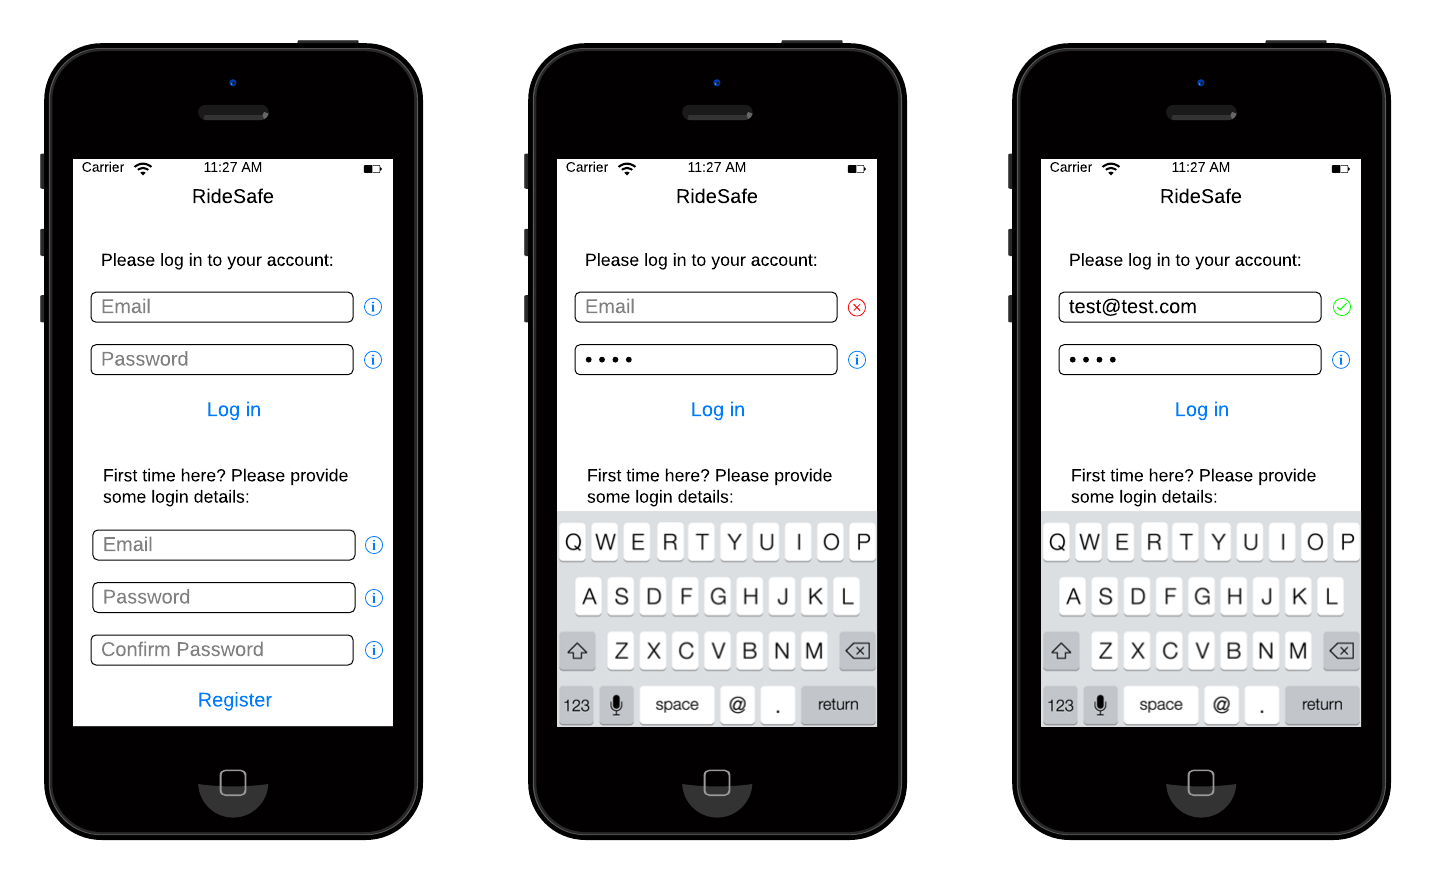
\includegraphics[scale=0.6]{figures/final_design/log_in}
\label{fig:login}
\caption{Final design of the log in screen}
\end{figure}
\begin{figure}[H]
\centering
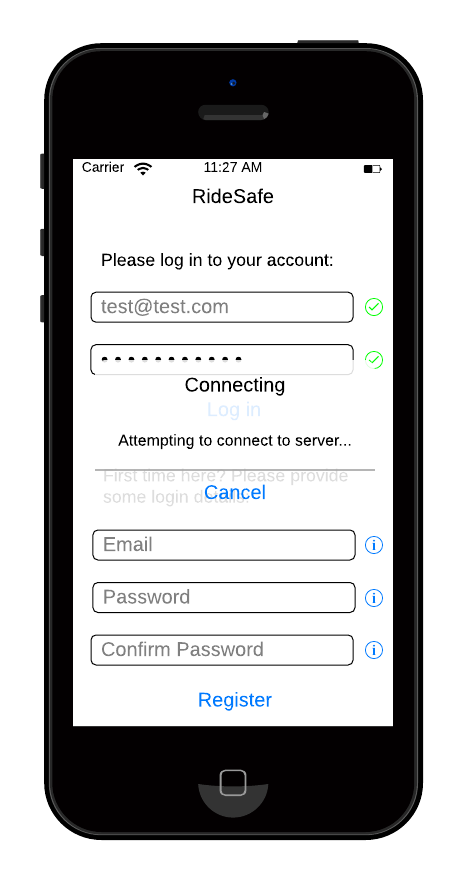
\includegraphics[scale=0.6]{figures/final_design/login_progress}
\label{fig:login}
\caption{The log in screen during log in, showing the user what is happening}
\end{figure}
\begin{figure}[h]
\centering
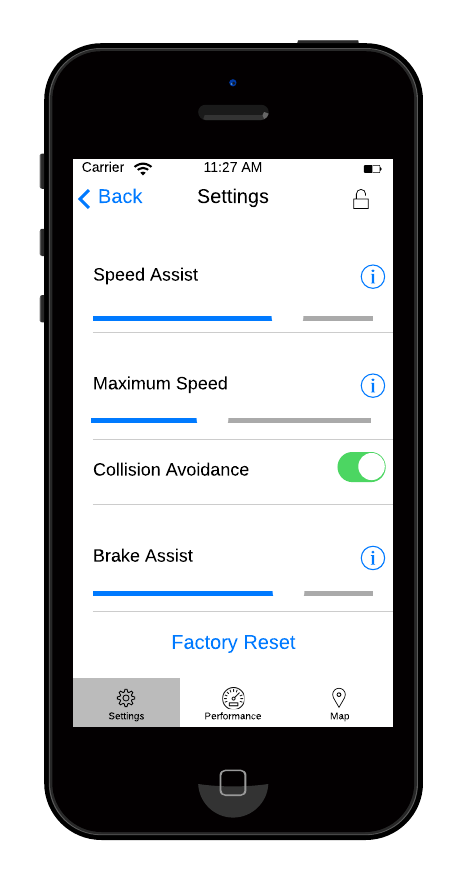
\includegraphics[scale=0.6]{figures/final_design/settings}
\caption{Final design of the settings screen}
\end{figure}
\begin{figure}[H]
\centering
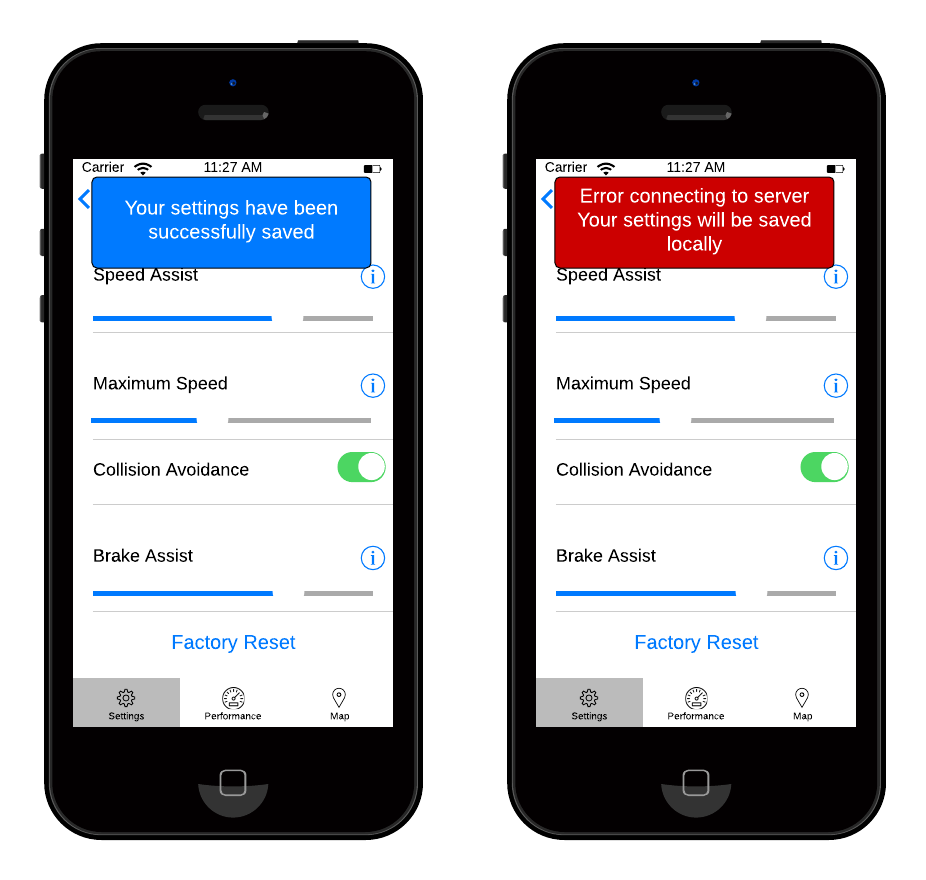
\includegraphics[scale=0.6]{figures/final_design/settings_notify}
\caption{Showing some of the notifications that may appear on the settings screen}
\end{figure}
\begin{figure}[h]
\centering
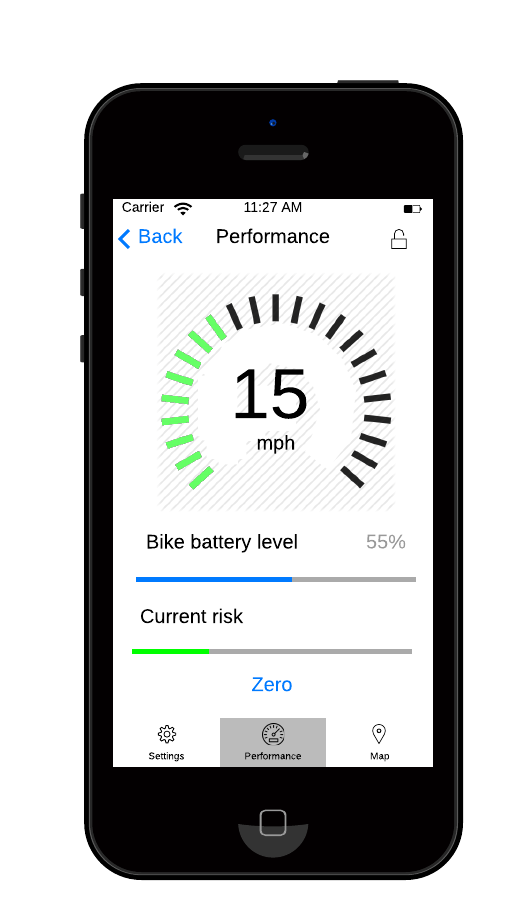
\includegraphics[scale=0.6]{figures/final_design/performance}
\caption{Final design of the rider performance screen}
\end{figure}

\section{Hardware Components Layout}
\begin{figure}[H]
\centering
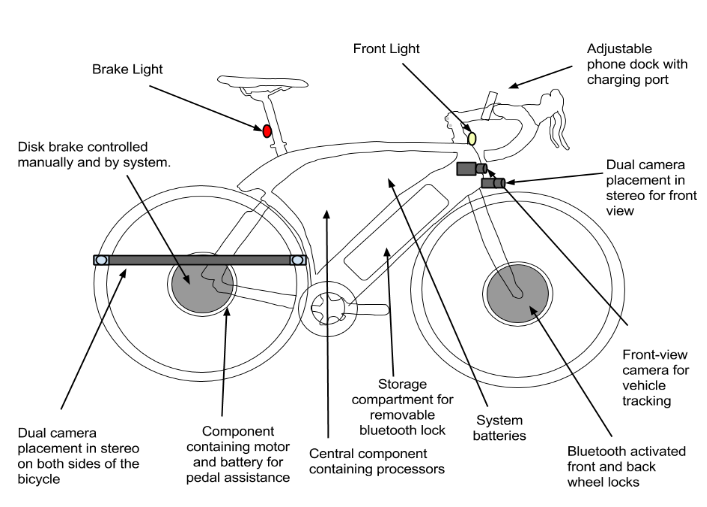
\includegraphics[scale=0.6]{figures/final_design/BicycleDrawing}
\caption{Final layout of hardware components on the bicycle}
\label{fig:final_layout}
\end{figure}

\begin{figure}[H]
\centering
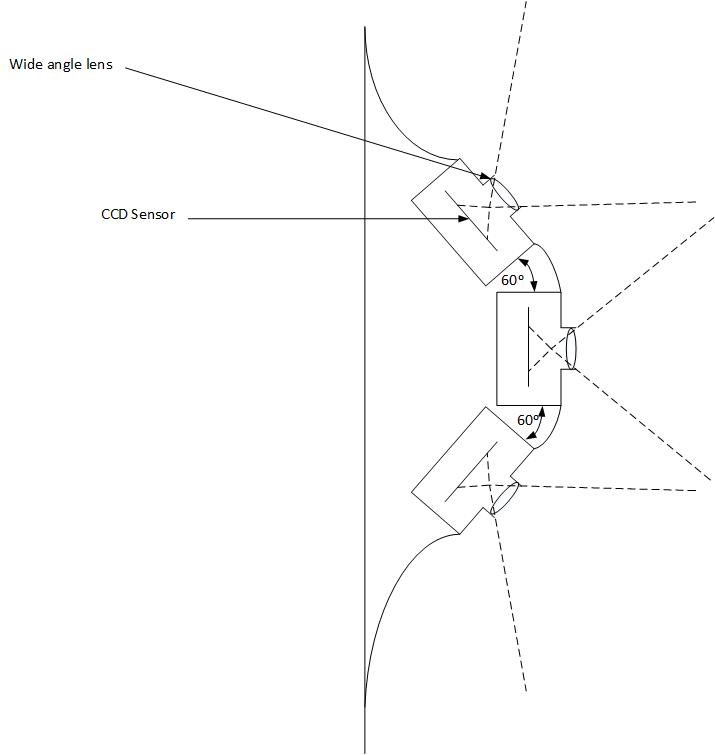
\includegraphics[scale=0.6]{figures/fan_camera}
\caption{Fan camera layout developed by Brauckmann \textit{et al.} \citep{towards_all_around_sensing}}
\label{fig:fan_camera}
\end{figure}

\paragraph{}We decided to use cameras as our primary sensor due to their robustness and affordability. Compared to using a laser range finder such as LIDAR, it seemed like the better option as it did not include moving parts that could easily break; which is an important feature to have when implemented on a bicycle as a bicycle is much more susceptible to wear and tear. The cameras on either side of the bike are positioned in stereo, while each camera is composed of a fan camera (shown in figure \ref{fig:fan_camera}). On the front of the bicycle, a single camera (again a fan camera) is used and placed higher up than the rest of the cameras (underneath the handlebars). This is for the bicycle to detect vehicles that are far in front of the bicycle. We decided not to use two cameras in stereo on the front of the bicycle; for one it would be obstructive for the cyclist to have two cameras sticking out on either side of the bicycle, but also the cameras would need to be positioned quite far apart in order to detect vehicles at a range. The stereo cameras on the front of the bicycle would also need to be placed further down on the bicycle in order to detect vehicles using the same algorithms as the other stereo cameras.

\section{Collision Avoidance System}
\begin{figure}[H]
\centering
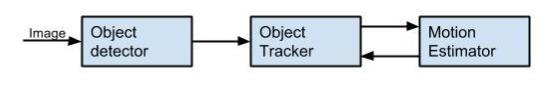
\includegraphics[scale=0.6]{figures/final_design/block_diagram_tracking}
\caption{Block Diagram for car tracking system (based on work by Zhao \textit{et al.}\cite{qualitative_car_tracking})}
\label{fig:block_diagram}
\end{figure}

There will be three steps towards a system that monitors nearby objects: detection, tracking and motion estimation. These steps will be described below.
\subsection{Detecting a vehicle and tracking}
\subsubsection{In Front of bicycle}
A single fan camera will be used to detect vehicles at range in front of the bicycle. In order for the bicycle to detect vehicles, we will first need to use an edge detector algorithm. The methods describe by Rosenfeld \textit{et al.} \citep{edge_detection} should work here. Using greyscale images, the system can detect edges by examining the average grey level of pairs of neighbouring pixels that meet at a point. The relative orientation of these neighbouring pixels will determine the orientation of the edges.

\paragraph{Exploiting Symmetry}
As decribed by Brauckmann \textit{et al.} \citep{towards_all_around_sensing} for the use of their system, we can adopt the method here. The system, with the use of an edge detection method described earlier, will detect edges and have vertical symmetry. This is because vehicles from behind tend to look symmetrical (see figure \ref{fig:cars_follow} for a demonstration). This is useful for the situation where the cyclist is behind cars in the same lane. The idea is to prevent the cyclist from hitting the back of any cars, maybe due to the cyclist being unaware that the vehicle in front has applied the brakes. The function for this method has been described by Zielke \textit{et al.} \cite{zielke1993intensity}. The vertical axis is very useful for measuring the vehicles lateral distance as nodding of the camera will not affect this method.

\begin{figure}[H]
\centering
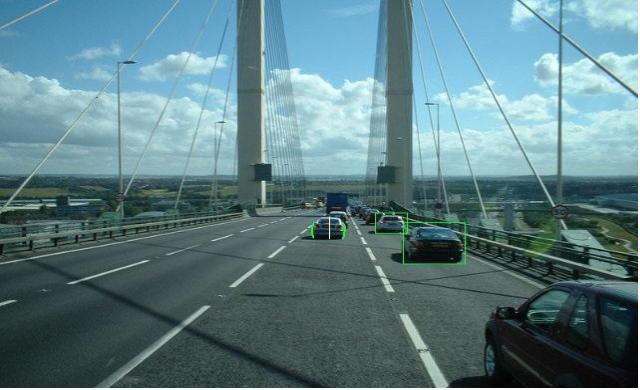
\includegraphics[scale=0.6]{figures/final_design/Car_follow_scenario}
\caption{What the system will see in a car following situation}
\label{fig:cars_follow}
\end{figure}

\paragraph{Local Orientation Coding and Neural Networks} This was a method used by Brauckmann \textit{et al.} in their car sensing system \citep{towards_all_around_sensing}. This method was developed by Goerick \& Brauckmann \citep{goerick1994local}. The main reason for using this technique is to provide flexiibility in the vehicle detection, so that the system is not too heavily reliant on exploiting symmetry. In order to use neural networks, an appropriate feature extraction process is needed. This is why we use a local orientation coding technique (described by Goerick \& Brauckmann \citep{goerick1994local}). The local orientation coding technique will then be used in combination with a lateral histogram technique. The local orientation histograms will contain guesses for the location of a vehicle in the image. A neural network classifier will then determine that the guesses do contain a vehicle. The neural network will need to be trained in detecting certain vehicle types with the use of sample images. An image of a van will allow detection of vans wheareas an image of a car will allow detection of cars. The image used to train the neural network can be of a low resolution so that it isn't so precise on detecting a vehicle of a certain type, so that it can detect a wider variety of vehicles.

\subsubsection{The sides of the bicycle}

\paragraph{}As mentioned previously, the sides of the bicycle will be monitored using cameras positioned in stereo. The method we will use is mostly based on the method used by Brauckmann \textit{et al.} \citep{towards_all_around_sensing} in their 'VisionBumper' system. This method is very useful because it is a simple method designed for a system not will not require the vehicle to plan its own trajectories. Our system will not plan its own trajectories but will only apply the brakes at appropriate times and warn the cyclist. This is because we found having a bicycle control itself will be a risk as the cyclist is required to balance the bicycle, and the cyclist may find it disorientating to have the bicycle control itself which may result in the cyclist falling of the bicycle and causing injury. 

\paragraph{}Using stereo fan cameras closer to the ground on either side of the bicycle, we can detect cars getting too close to the bicycle. Having the cameras monitor the road we are able to detect a vehicle obscuring the view. In order to get images that can be determined by the system, we will need to use a process called Inverse-perspective
mapping (for implementation, see paper \cite{inverse-perspective_mapping}). This will formulate a viewable image for the system from information gathered from the multiple CCD sensors. 

\paragraph{}The position of the cameras on either side of the bicycle should provide almost 360 degree coverage around the bicycle. This will act as a 'safe zone' around the bicycle (see figure \ref{fig:safe_zone}). If a vehicle enters this safe zone, the system will have time to react. If an object obscures the road in the image gets to a certain distance away from the bicycle, the bicycle will apply the brakes accordingly. In a situation where a car enters the cyclists lane or tries to overtake in a reckless way, applying the brakes will allow the vehicle to drive past with the cyclist unharmed.

\paragraph{}Although we are using a stereo camera system, we will not be using optical triangulation to measure the distance of objects. This is because the system not be able to reliably obtain two corresponding image locations of the same surface point of an object in 3D. Instead, the system will detect distortions in the processed image (obtained using inverse-perspective mapping) from both cameras. The view from the cameras should be a ground view of the road, and as a vehicle enters the bicycles 'safe zone' the cameras will pick up two different images of the object (due to being at different angles to the vehicle). The distortions in the final image after using inverse-perspective mapping will be considered possible object locations. The problem with this approach is that the cameras should not view too far out as this method requires the cameras to be constantly viewing the road, also viewing too far out will cause the bicycle to brake too early or brake when not needed.

\begin{figure}[H]
\centering
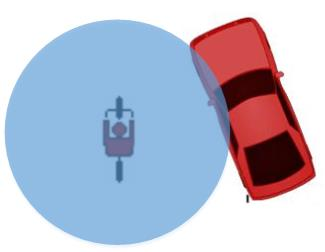
\includegraphics[scale=0.6]{figures/final_design/bicycle_safe_zone}
\caption{Image showing the typical coverage the side cameras should give}
\label{fig:safe_zone}
\end{figure}

\subsection{Estimating distance and speed}
In our system, distance and speed all comes down to the size of the object being tracked over time. 

\chapter{Conclusion}
In conclusion, we have designed a product that we feel commuting cyclists will be able to use for their commute to work. We think that this product will be able to significantly improve safety for users of our product, but furthermore other cyclists will feel the benefit due to the Safety in Numbers concept.

In the early stages we considered a whole range of possible ideas and ways in which we could tackle this problem but in the ended we decided to go with an approach based around automated braking and collision detection. This mirrors similar technology found in cars - particularly the Blind Spot technology developed by Infiniti. We were very happy with this decision as it meant we were able to design a versatile product that be believe will work well.

This product could form the basis of a smart bike in the future and we think that there are many ways in which our design could be expanded. It could be expanded to include more automation but perhaps more simply the app could be developed further to monitor more features of the bike and enable more settings to be tweaked. 

The mobile app is something that works particularly well with this format because of it's versatility and in particular it could allow us to revisit the Google Glass idea that we considered in the early stages - once this technology becomes more developed.

\part*{Appendices}

\appendix
\chapter{Research Report}
In this mini-report we will be showing the preliminary research that we did before designing our final solution. The overall aim of doing this research was to discover what was currently going wrong in cycling and where we could improve it. 

We did this by analysing a range of statistics and then looking at the cycling safety products past \& present to see what has succeeded and what has failed and also is possible we have tried to analyse the reasons why. 
\newpage
\section{Accidents}
\subsection{Weather Conditions}
During the winter months, new hazards occur and visibility of the cyclist is poorer. In the UK, slipping on ice is the most common cause of non-collision accidents, contributing 26\% of these accidents; 8\% happen on wet roads, being the second most common \citep{winter_safety}. Potholes account for 3\% of non-collision injuries and mechanical failures account for 2.5\% \citep{non-collision_casestudy}.

%According to the most recent National Travel Survey statistics (2013) \textbf{43\% of the population owns a bicycle} 

\subsection{Casualties}
\begin{table}[H]
\begin{tabular}{| l | l | l | l |}
\hline
 & \textbf{Child} & \textbf{Adult} & \textbf{All} \\ \hline
 Killed & 6 & 103 & 109 \\ \hline
 Seriously Injured & 276 & 2867 & 3143 \\ \hline
 Slightly Injured & 1676 & 14510 & 16186 \\ \hline
 Total & 1958 & 17480 & 19438 \\ \hline
\end{tabular}
\caption[Table caption text]{Cyclist casualties reported to the police in 2013 \citep{cycling_accidents}}
\label{table:casualties}
\end{table}

\paragraph{}Every year, there are around 19000 of reported cases of cyclists being killed or injured. However these are only cases that are reported to the police. This does not take into account cyclists in accidents not on the road, and there are many cases of cyclist injuries not being reported to the police, even when seriously injured and taken to hospital \citep{cycling_accidents}.
A much larger portion of accidents occur with adults rather than children. This gives us reason to develop a bicycle system which focuses mostly on adult cyclists, but will aim to be usuable for a broader audience. 
\subsection{Road types}
\paragraph{}The Royal Society for the Prevention of Accidents \cite{cycling_accidents} mention that most cycling accidents happen in urban areas. Almost two thirds of cyclists that are killed or seriously injured have the accidents happen around a road junction, with T-junctions bein the most commonly involved. It also mentions that roundabouts are particularly dangerous junctions. The severity of injuries increases with the speed limit applied to the road. Although more accidents happen on urban roads (75\%), half of cyclist deaths occur on rural roads. The Royal Society for the Prevention of Accidents \cite{rural_road_safety} also suggest this may be due to the nature of rural roads having more bends while also having fewer facilities for cyclists. This means that our system should apply to rural roads as well as urban roads, by not just focusing on situations that only happen on urban roads. 
\subsection{Time of day}
\paragraph{}Around 80\% of accidents occur in daylight \citep{cycling_accidents}. The most dangerous hours for cyclists are between 3:00pm to 6:00pm and 8:00am to 9:00am. These are typical commuting hours where road traffic is greater, which would mean that commuters are more prone to accidents. So our system should focus towards this audience. However, cycling accidents are more likely to be fatal while it is dark. Which would mean our system should provide sufficient visibility to accomodate this.
\subsection{Types of accident}
\subsubsection{Accidents involing no collisions}
\paragraph{}These types of accident are cause by the cyclist loosing control of the bicycle. These contribute to around 16\% of fatal or serious cyclist accidents \citep{cycling_accidents}. 

\subsubsection{Collision between bicycle and vehicle}

The most common cause of this type of accident is either the cyclist or vehicle driver failing to look properly \citep{cycling_accidents}. At junctions, drivers contribute 57\% of accidents where someone failed to look properly and for cyclists it is 43\%

\paragraph{Drivers that cause the accidents}. Factors where drivers cause these accidents include poor manoeuvres (17\%) and careless or driving in a hurry (17\%). Drivers are also more likely to cause accidents when speeding, driving under the influece of alcohol or travelling too fast for the road conditions.

\paragraph{Cyclists that cause the accidents}In the case of cyclists causing collisions, 20\% of serious collisions are caused by cyclists entering the road from a pavement.
 
\paragraph{} Cars or taxis are more likely to be involved in collisions. In most cases, the cyclist is hit by the front of the vehicle. Although most cases are caused by drivers, cyclists contribute a significant portion. So the system should be required to prevent these types of accident caused by both vehicle driver and cyclist.


\newpage
\section{Questionnaires}
\subsection{Cyclists Questionnaire}
We started out by contacting cyclists directly, this was to see how they had interpreted the 
\begin{figure}[H]
\centering
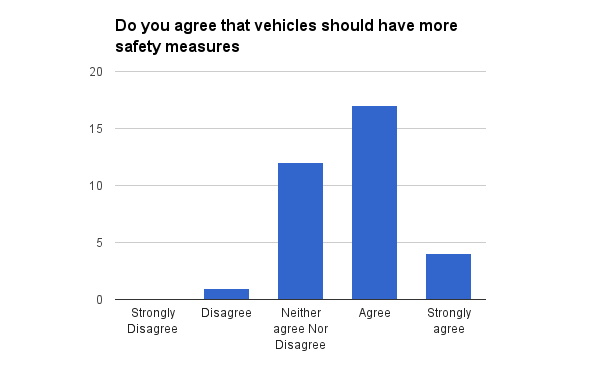
\includegraphics[scale=0.6]{figures/research_report/questionnaires/drivers_1}
\end{figure}
\begin{figure}[H]
\centering
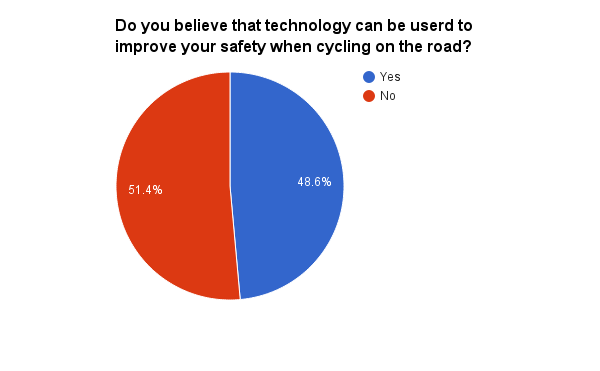
\includegraphics[scale=0.6]{figures/research_report/questionnaires/drivers_2}
\end{figure}
It was encouraging for us to see that most cyclists actually agreed that there should be more safety measures in cycling, this indicates that they may well be open to using whatever we end up designing. Also roughly 50\% of people then also said that they thought technology could be used which may well be the route we end up going, since most modern problems can be solved using technology. It is also worth us considering the 50\% of people who did not think technology is a viable option and seeing what their suggestions are.
\begin{figure}[H]
\centering
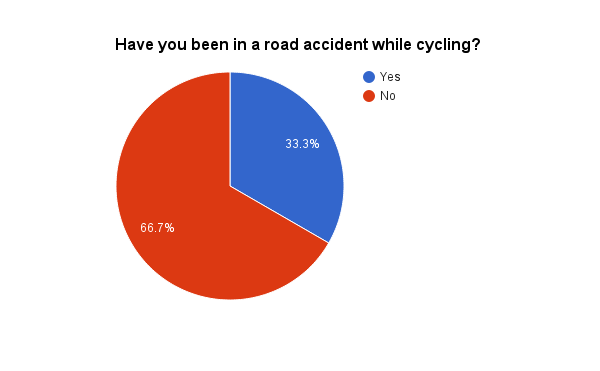
\includegraphics[scale=0.6]{figures/research_report/questionnaires/drivers_3}
\end{figure}
It was quite surprising to learn that $\frac{1}{3}$ of cyclists that we spoke to have been involved in an accident. This is quite  a bit higher than we were expecting but strongly indicates that we were right in saying that safety is a major problem in the cycling world.
\begin{figure}[H]
\centering
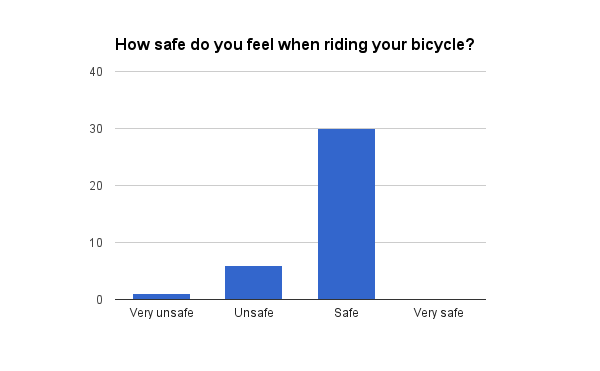
\includegraphics[scale=0.6]{figures/research_report/questionnaires/drivers_4}
\end{figure}
Following on from the previous question it was actually strange that the vast majority of people actually said they felt safe while riding their bicycle. It is possible that the wording of the question `your bicycle' enticed people to say they felt safe. Nevertheless this was surprising and it's probably worth talking to non-cyclists to see whether they think that cycling is a safe activity. This could also show that many current cyclists would be reluctant to part with their bicycle and maybe an add-on component would be more appealing.
\begin{figure}[H]
\centering
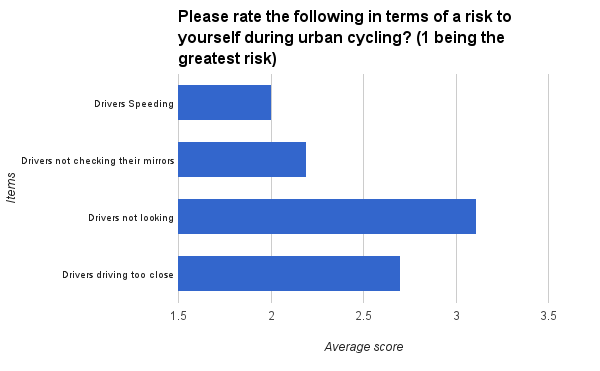
\includegraphics[scale=0.6]{figures/research_report/questionnaires/drivers_5}
\end{figure}
In truth this question didn't give us too much information, all of the answers ended up roughly similar. The top two responses though were `Drivers not looking' and `Drivers driving too close' this tells us some of the types of things that cyclists find dangerous and that we could try to cut out to improve safety, and the perception of safety.
\begin{figure}[H]
\centering
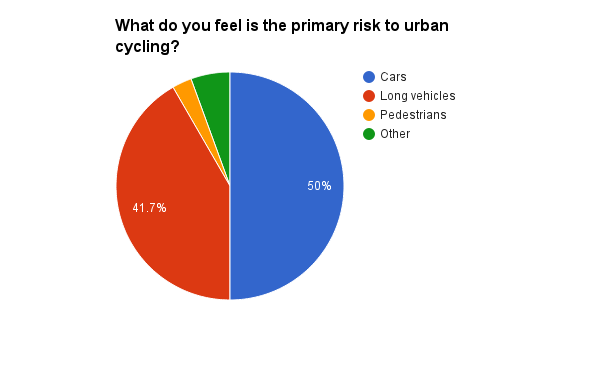
\includegraphics[scale=0.6]{figures/research_report/questionnaires/drivers_6}
\end{figure}
The answer to this question was very clear, cyclists feel that it is the motorised vehicles (cars, buses and lorries) on the road which pose the biggest risk. This is useful information because it really tells us where to focus. This becomes particularly important if we decide to use some sort of technology that involves communication between bikes and the other road users.
\begin{figure}[H]
\centering
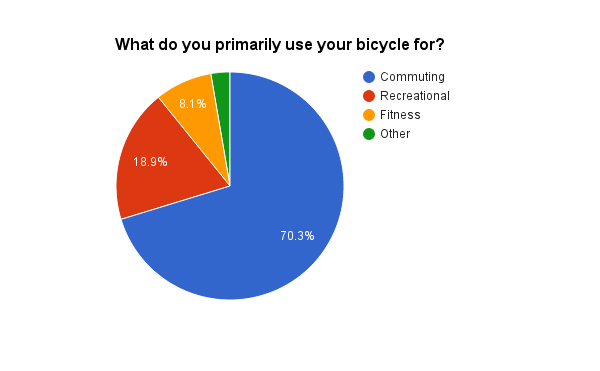
\includegraphics[scale=0.6]{figures/research_report/questionnaires/drivers_7}
\end{figure}
This was not particularly surprising, but this helped us to focus our efforts more closely on the actual group of cyclists who would be most affected. It is probably best for our product that it reaches as many people as possible, also our prior research shows that commuters are one the groups most at risk.
\begin{figure}[H]
\centering
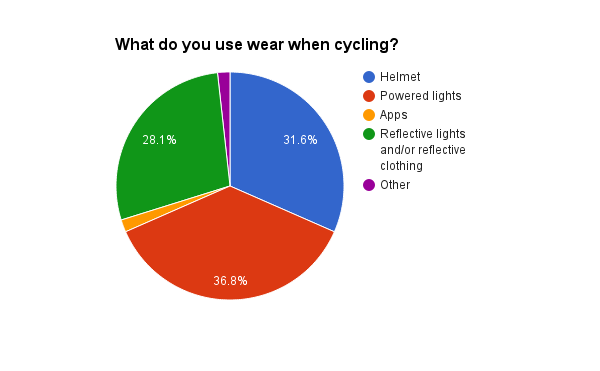
\includegraphics[scale=0.6]{figures/research_report/questionnaires/drivers_8}
\end{figure}
This pretty much represented what we were expecting  - most cyclists do use lights (as required by law) and probably the more serious ones will also wear reflective clothing, it was surprising to see how many people actually do use helmets as this does not really reflect what was generally observed by looking at cyclists in the street. We were not surprised to learn that hardly anyone at all actually use apps or any other specialised equipment. 
This may indicate a gap in the market, but could also indicate cyclists resistance to newer technology.
\subsection{Car Drivers Questionnaire}
We also spoke to car drivers because we wanted to see firstly how easy it might be to get them on board with our product, and also to get their viewpoint of the major risks on the road.
\begin{figure}[H]
\centering
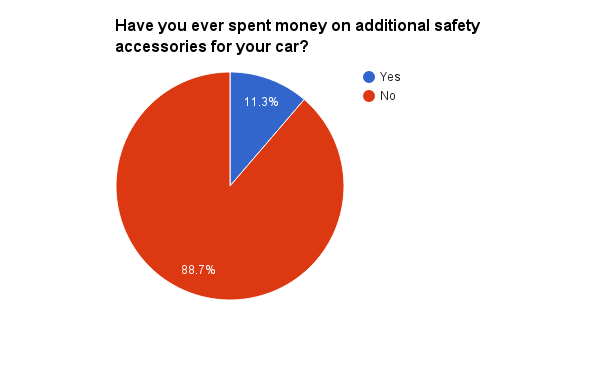
\includegraphics[scale=0.6]{figures/research_report/questionnaires/cars_1}
\end{figure}
This was quite an alarming response - only 11\% of respondents have actually spent money on additional safety accessories for their car, and in fact out of these only 1 had spent upwards of \pounds50. It can be safely assumed that drivers would be even less willing to spend money on a safety product that is primarily to aid cyclists.

It is possible that there could be some sort of free package that drivers would be willing to adopt to aid cyclists (and general road safety).

\begin{figure}[H]
\centering
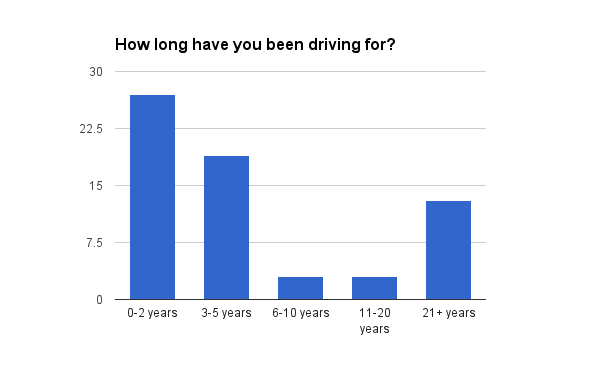
\includegraphics[scale=0.6]{figures/research_report/questionnaires/cars_7}
\end{figure}
\begin{figure}[H]
\centering
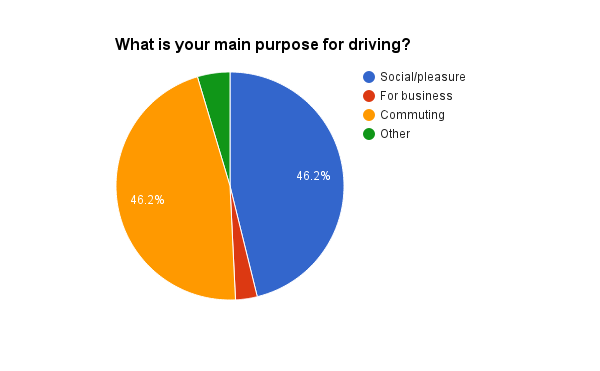
\includegraphics[scale=0.6]{figures/research_report/questionnaires/cars_6}
\end{figure}
Roughly 50\% of drivers main purpose for driving is for commuting - this along with the similar question for cyclists reinforces the position that commuting should be the main target for our product.
\begin{figure}[H]
\centering
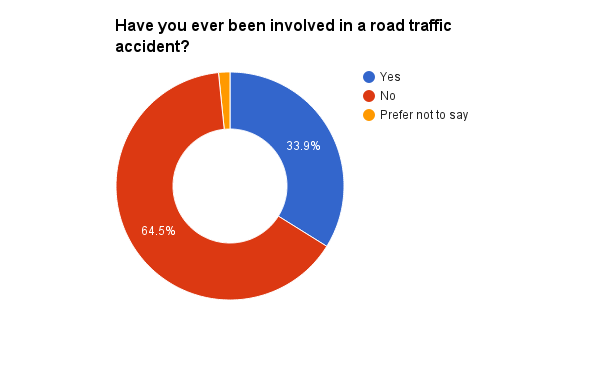
\includegraphics[scale=0.6]{figures/research_report/questionnaires/cars_8}
\end{figure}
This figure was almost identical to that of cyclists which was equally as surprising and could potentially mean that cyclists are in fact no more at risk than anybody else on the road. This would be bad if we continued to go down the route of cycling safety.
 
\begin{figure}[H]
\centering
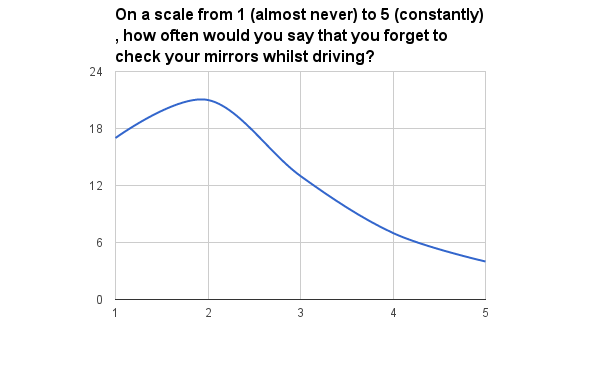
\includegraphics[scale=0.6]{figures/research_report/questionnaires/cars_3}
\end{figure}
In this question we were trying to figure out how much to blame car drivers were for accidents involving them and cyclists. We had to be careful with the wording of this question since people are likely to say that their driving is perfect and they are never to blame. This means that in reality we can probably shift this whole graph over to the right slightly. Even taking the values as they are over 5\% of the respondents said that they constantly forget to check their mirrors while driving.
\begin{figure}[H]
\centering
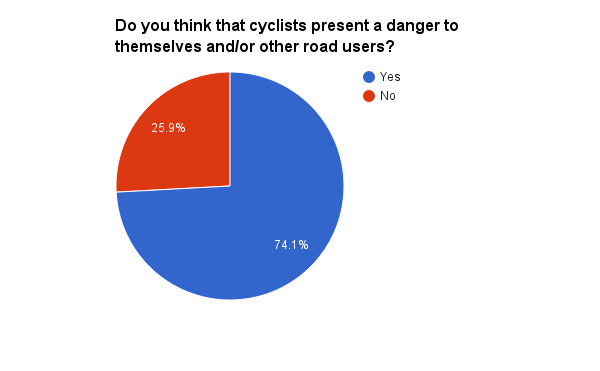
\includegraphics[scale=0.6]{figures/research_report/questionnaires/cars_2}
\end{figure}
\begin{figure}[H]
\centering
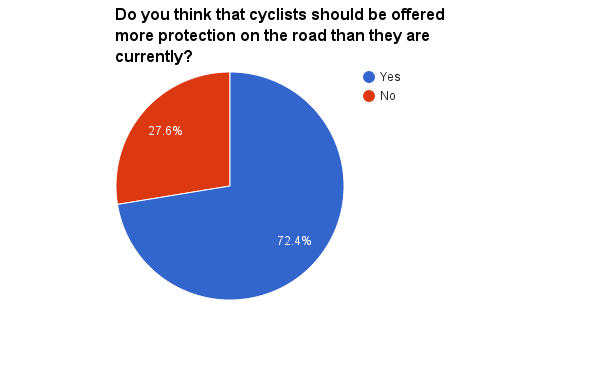
\includegraphics[scale=0.6]{figures/research_report/questionnaires/cars_4}
\end{figure}
As expected the answers to both of the above questions were fairly similar and shows that drivers recognise the risk that cyclists pose and actually think cyclists do need more protection. This is encouraging if we did want to incorporate drivers into our solution somehow.
\begin{figure}[H]
\centering
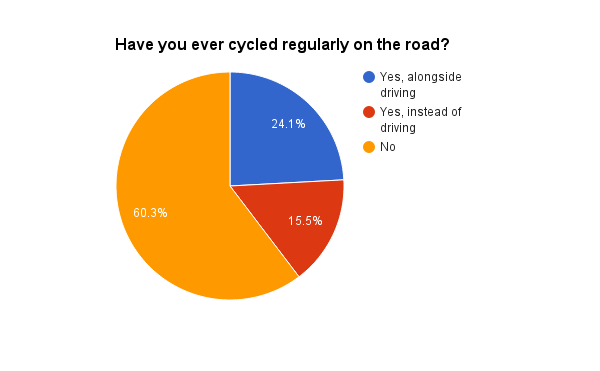
\includegraphics[scale=0.6]{figures/research_report/questionnaires/cars_5}
\end{figure}
This shows a potential lack of understand/empathy for cyclists from drivers. Most of them have never cycled regularly on the road and so probably do not know the problems that cyclists face. This could mean that our product should work independent of drivers input. 

\newpage
\section{Current products}
We looked at a whole variety of safety products currently on the market for cars and trucks as well as bikes. The reason for this was to see why certain products were succeeding and which features of these products we might wish to incorporate into our solution. We also looked at failed products to get an idea of the potential design problems we might encounter later on as well as allowing us to rule out some of the previously attempted solutions.
\subsection{Bike Lights}
The most basic, and often the only, form of bike safety used is the bike light; this is used to make a cyclist visible to all road users allowing them to take the appropriate action. In the UK front and rear bike lights (and reflectors) are required by law between sunset and sunrise. This is governed by the Road Vehicle Lighting Regulations 1989\cite{rvlr} and if our solution were to use in-built lighting we would have to make sure that we complied with these regulations. This poses an interesting problem because different sets of regulations exist in different countries; most manufacturers actually tend to ignore the UK's regulations because of the relatively small cycling population and also the regulations are considered by many to be old and outdated. In practice as long as a cyclist has lights of some description on both the front and rear of their bike they are unlikely to be questioned by police. 

Bike lights come in many different forms but, according to retailer that we spoke to, LED currently dominates the market. They are small, cheap, last forever and they provide a lot of light! The retailer also told us that it is important for lights to have a wide field as well as to be bright. This allows cyclists to be seen even by people not directly in front or behind; for example cars waiting to pull out of a junction.

\paragraph{Revolight} A slightly different take on the bike light is the Revolight\cite{revolight}; here the light is incorporated the bike's tyres. The lights are mounted all around the wheel and are timed to only illuminate when facing the front or rear of the bicycle using a fork-mounted magnet and integrated accelerometer. The primary benefit of this is that it gives total 360\degree vision of the bike.

This started as a Kickstarter project\cite{revo_ks} in 2011 and has since reached it's goal and is now on sale for \$199. There is no sales information readily available nor any statistics about how operationally successful this product has been. However the Revolight design has won several awards from cycling publications\cite{revo_awards} and has recently received \$1 million in funding from investors so it appears that this product has been very successful.

\paragraph{Blaze Laserlight}
The Blaze Laserlight\cite{laserlight} projects a green laser image of a bicycle up to 6m ahead of the cyclist. The idea of this product is to cut down on accidents where the cyclist is caught in a vehicles blind spot at the time of them making a manoeuvre into their path. According to the creators of the Blaze Laserlight - 79\% of accidents happen this way. 

One particular design decision that was made by the people at Blaze was to have the light project in green, the reason for this is because humans are most sensitive to light between 490-560 nm (green light). This could be something to think about if we incorporate lights into our design.

This product tries to avoid accidents by making other road users more aware of cyclist. However it has a few problems:
\begin{itemize}
\item It will not be as effective at night. This technology is based on LED bike lights which are only effective in low light.
\item It still puts the responsibility on other road users. It will not protect the cyclist from unobservant road users and it most likely these people who are causing these accidents in the first place.
\end{itemize}

\paragraph{XFire}
The XFire\cite{xfire} product works similarly to the Blaze Laserlight by projecting light onto the road. However instead of projecting an image of the bike it projects a bike lane. The idea here is to buy cyclists more space during overtaking manoeuvres, particularly on roads where there is no cycle lane. This has the added advantage that all road users are familiar with bike lanes and how they operate. 

This product is relatively cheap, retailing online at \$29.99 however has the same disadvantages as the Blaze Laserlight

\subsection{Helmets}
Probably the next most common safety product used at the moment is the helmet. The helmet is a impact reduction approach to managing the risk; it will not help to prevent an accident from occurring but it may stop an accident from being fatal. Currently helmets are not required by UK law however according to government guidelines, ``You \textit{should} wear a cycle helmet which conforms to current regulations, is the correct size and securely fastened"\cite{helmet_gov}.

\paragraph{Hovding airbag}According to, former professional cyclist, Michael Hutchinson ``The most outstanding design flaw with the traditional polystyrene helmet is that it messes up people's hair, it's sweaty on the head, also a lot of people don't like the look of bike helmets."\cite{hutch} The ``Hovding airbag" \cite{hovding} is an invisible helmet that attempts to overcome these issues. It is an airbag fitted into a neck collar and uses sensors and an algorithm to detect a fall. Once detected, it inflates over the user’s head like a hood, protecting the users head from impact damage.

This has been the only noticeable innovation in bike helmets and for this reason it is unlikely that helmets will form and significant part of our solution. However, this particular product does show the importance of style as well as safety and that it something we will need to keep in mind throughout the design process.

\subsection{Mobile apps}
Mobile apps are now used throughout everyday life due to their accessibility and ability to interact with the outside world. This ability to interact might be something that we can utilise in our product. Here we looked at some of the ways in which mobile apps are currently being used by cyclists.

\paragraph{Bike Doctor} One example of such an app is the `Bike Doctor'\cite{bike_doctor} which is supposed to be a personal bike mechanic. It contains many bike maintenance guides and is designed to provide easy to follow instructions on how to repair and maintain particular parts of the bicycle yourself. It was designed to be ideal for beginners but also as a handy reference guide for more experienced cyclists. This concept may be something to consider as it is a trusted app by over 14,000 cyclists and having a well maintained bike would prevent a chance of a breakdown during cycling and causing an injury during cycling. 

Something that this app does not do is detects faults in the bike to give tailored advice, similarly to the dashboard lights in cars. This would be a very useful feature that would improve bike safety. A problem with this app is that it will not prevent accidents that are not the fault of the cyclist; which our earlier research showed are the majority.

\paragraph{Strava} A particularly successful app that is used by cyclists is Strava\cite{strava}. Strava is predominantly a tracking application/social network where users can share their routes with other cyclists. A feature of Strava that we found particularly interesting was the in built challenges, where users earn recognition amongst their peers for cycling a particular distance or route. This really encourages people to cycle and moreover to keep up their cycling habit. Strava also has potential safety benefits because users can use recommended routes which should be safer to ride, however this is not the primary focus of Strava.

It does seem that the primary audience of this app is people who cycle for recreation or fitness, whereas we are predominantly targeting people who cycle for commuting or transport. However, it may be possible to overcome this problem by analysing routes of all cyclists to find the best possible routes to a given location.

\subsection{Smart Wheels}
The smart wheel is an idea to make commuting easier. The prime example of this is a product called the 'FlyKly Smart Wheel'\citep{flykly}. This wheel fits on any bicycle and includes a 250W motor,  torque sensor, motion sensor, temperature sensor and system monitoring sensors linked to a battery to provide an easier and more automatic cycle. The wheel can assist the cyclist up to 25km/h. The wheel also allows bluetooth connectivity to a mobile phone to show the user their performance and provide the ability for the user to change how much their wheel affects how much they cycle. The wheel also allows the user to lock the wheel in place with a motor lock with pin for improved safety.

\subsection{Wearable Technology}
Wearable technology is a trending topic and is likely to be more popular in the future. But as of now, very few people own any wearable technology and stick to using a mobile phone. Research into wearable technology was conducted just in case we were to incorporate any wearable technology into our system. 

\paragraph{Google Glass}
Google Glass \citep{google_glass} is a system embedded into the frame of a pair of glasses. It projects information onto the lens of the glasses so that it displays information directly to the users eyes. It also includes a camera is record what the user can see. All the functions performed by Google Glass are activated using voice, making it perform completely hands free.
However, there are many concerns with use of Google Glass; the biggest concern has to be privacy \citep{google_glass_privacy} as it is hard to determine whether someone is recording you using the glasses. Also many people believe the glasses can be an easy distraction, which is a big factor to take into account when designing our system if we consider to integrate it into Google Glass.

\paragraph{Pebble}
Pebble \citep{pebble} is a system embedded into a watch. The design of this watch is to keep simplicity and provide functionality. It uses a black and white 'e-paper' display to allow easy readability in daylight. It is very water resistant up to 50 meters and uses an optical hard coating to make it scratch resistant. The watch links to a mobile phone via bluetooth to provide notifications which gives it a variety of uses. The pebble can be used as a fitness tracker and can be linked to mobile fitness apps on the mobile phone. This would be useful on a bike as the strap allows the user to strap the watch to the handlebars of the bicycle and use it to display the users performance as they cycle.

\newpage
\section{Economy}
In a British Cycling Economy report \citep{british_economy_report}, it explains that cycling accessories contribute to over half the amount to the UK economy than the sales of bikes themselves. Typically bought accessories include helmets, locks and pumps as these are considered “necessary”. Also it mentions that interviews with commuters who cycle revealed that fear of theft and improper storage at their commute destination affects their choice in purchasing a bike; this has been influencing a growth in the investment of folding bicycles. Commuters also typically purchase safety clothing with their bicycle (ie, gloves and reflective gear). 

On average, Commuters spend £195 on bike accessories whereas recreational cyclists spend on average £70. Enthusiasts however spend on average £1,295 on accessories, which is more than their average spent on bicycles themselves at £1,200 (with a range spanning £600 - £1,600). These values will need to be taken into account when calculating the cost of the final product during the design phase. 

We may consider implementing the use of “necessary” items in our project in order to spread the use of the final product. We may also need to consider how to make our final product theft proof, while also making it compact and easy to store or carry to encourage its use.

\newpage
\section{Car technologies}
We looked at many different technologies, both emerging and established, that are in use in cars. This provided lots of inspiration and helped us to analyse what might work (and also what might not). Car technologies provide us with lots of information because they are much more developed that bike technologies and also there is a very wide user base. Also it is possible that the best way to improve safety in cycling to tackle the problems with drivers rather than cyclists.
\subsection{Blind spot technology}
An emerging technology that is particularly relevant to cyclists is blind spot technology Many car manufacturers are currently developing their own versions of the same idea - to check blind spots for the driver before they make a manoeuvre and alert them to any potential problems. It is clear to see how this is relevant to cyclists, as it is not uncommon for them to be caught in a drivers blind spot while over/undertaking. Here we will look at some of the different implementations of this and try and see what works well and what doesn't work so well.
\subsubsection{Volvo BLIS}
Volvo were one of the pioneers of this technology - introducing the initial version of their Blind Spot Information System in 2005\cite{volvo_blis}. This version worked using a camera mounted on the underside of both wing mirrors and then some image processing was done to identify things that looked like a car. This would take 25 images per second and then analyse the differences between successive frames. For an early system it worked quite well, however it did not work in all conditions - in particular heavy fog or snow. Also when travelling significantly faster or slower than the vehicle in question; however this may not be as big of a problem as it seems since when there is a significant speed differential the vehicle is likely to move out of your blind spot fairly quickly. Perhaps more alarmingly, especially from a user experience point of view, is that some users said that the technology would often identify up parked cars. 

\begin{figure}[h]
\label{fig:volvo_blis}
\centering
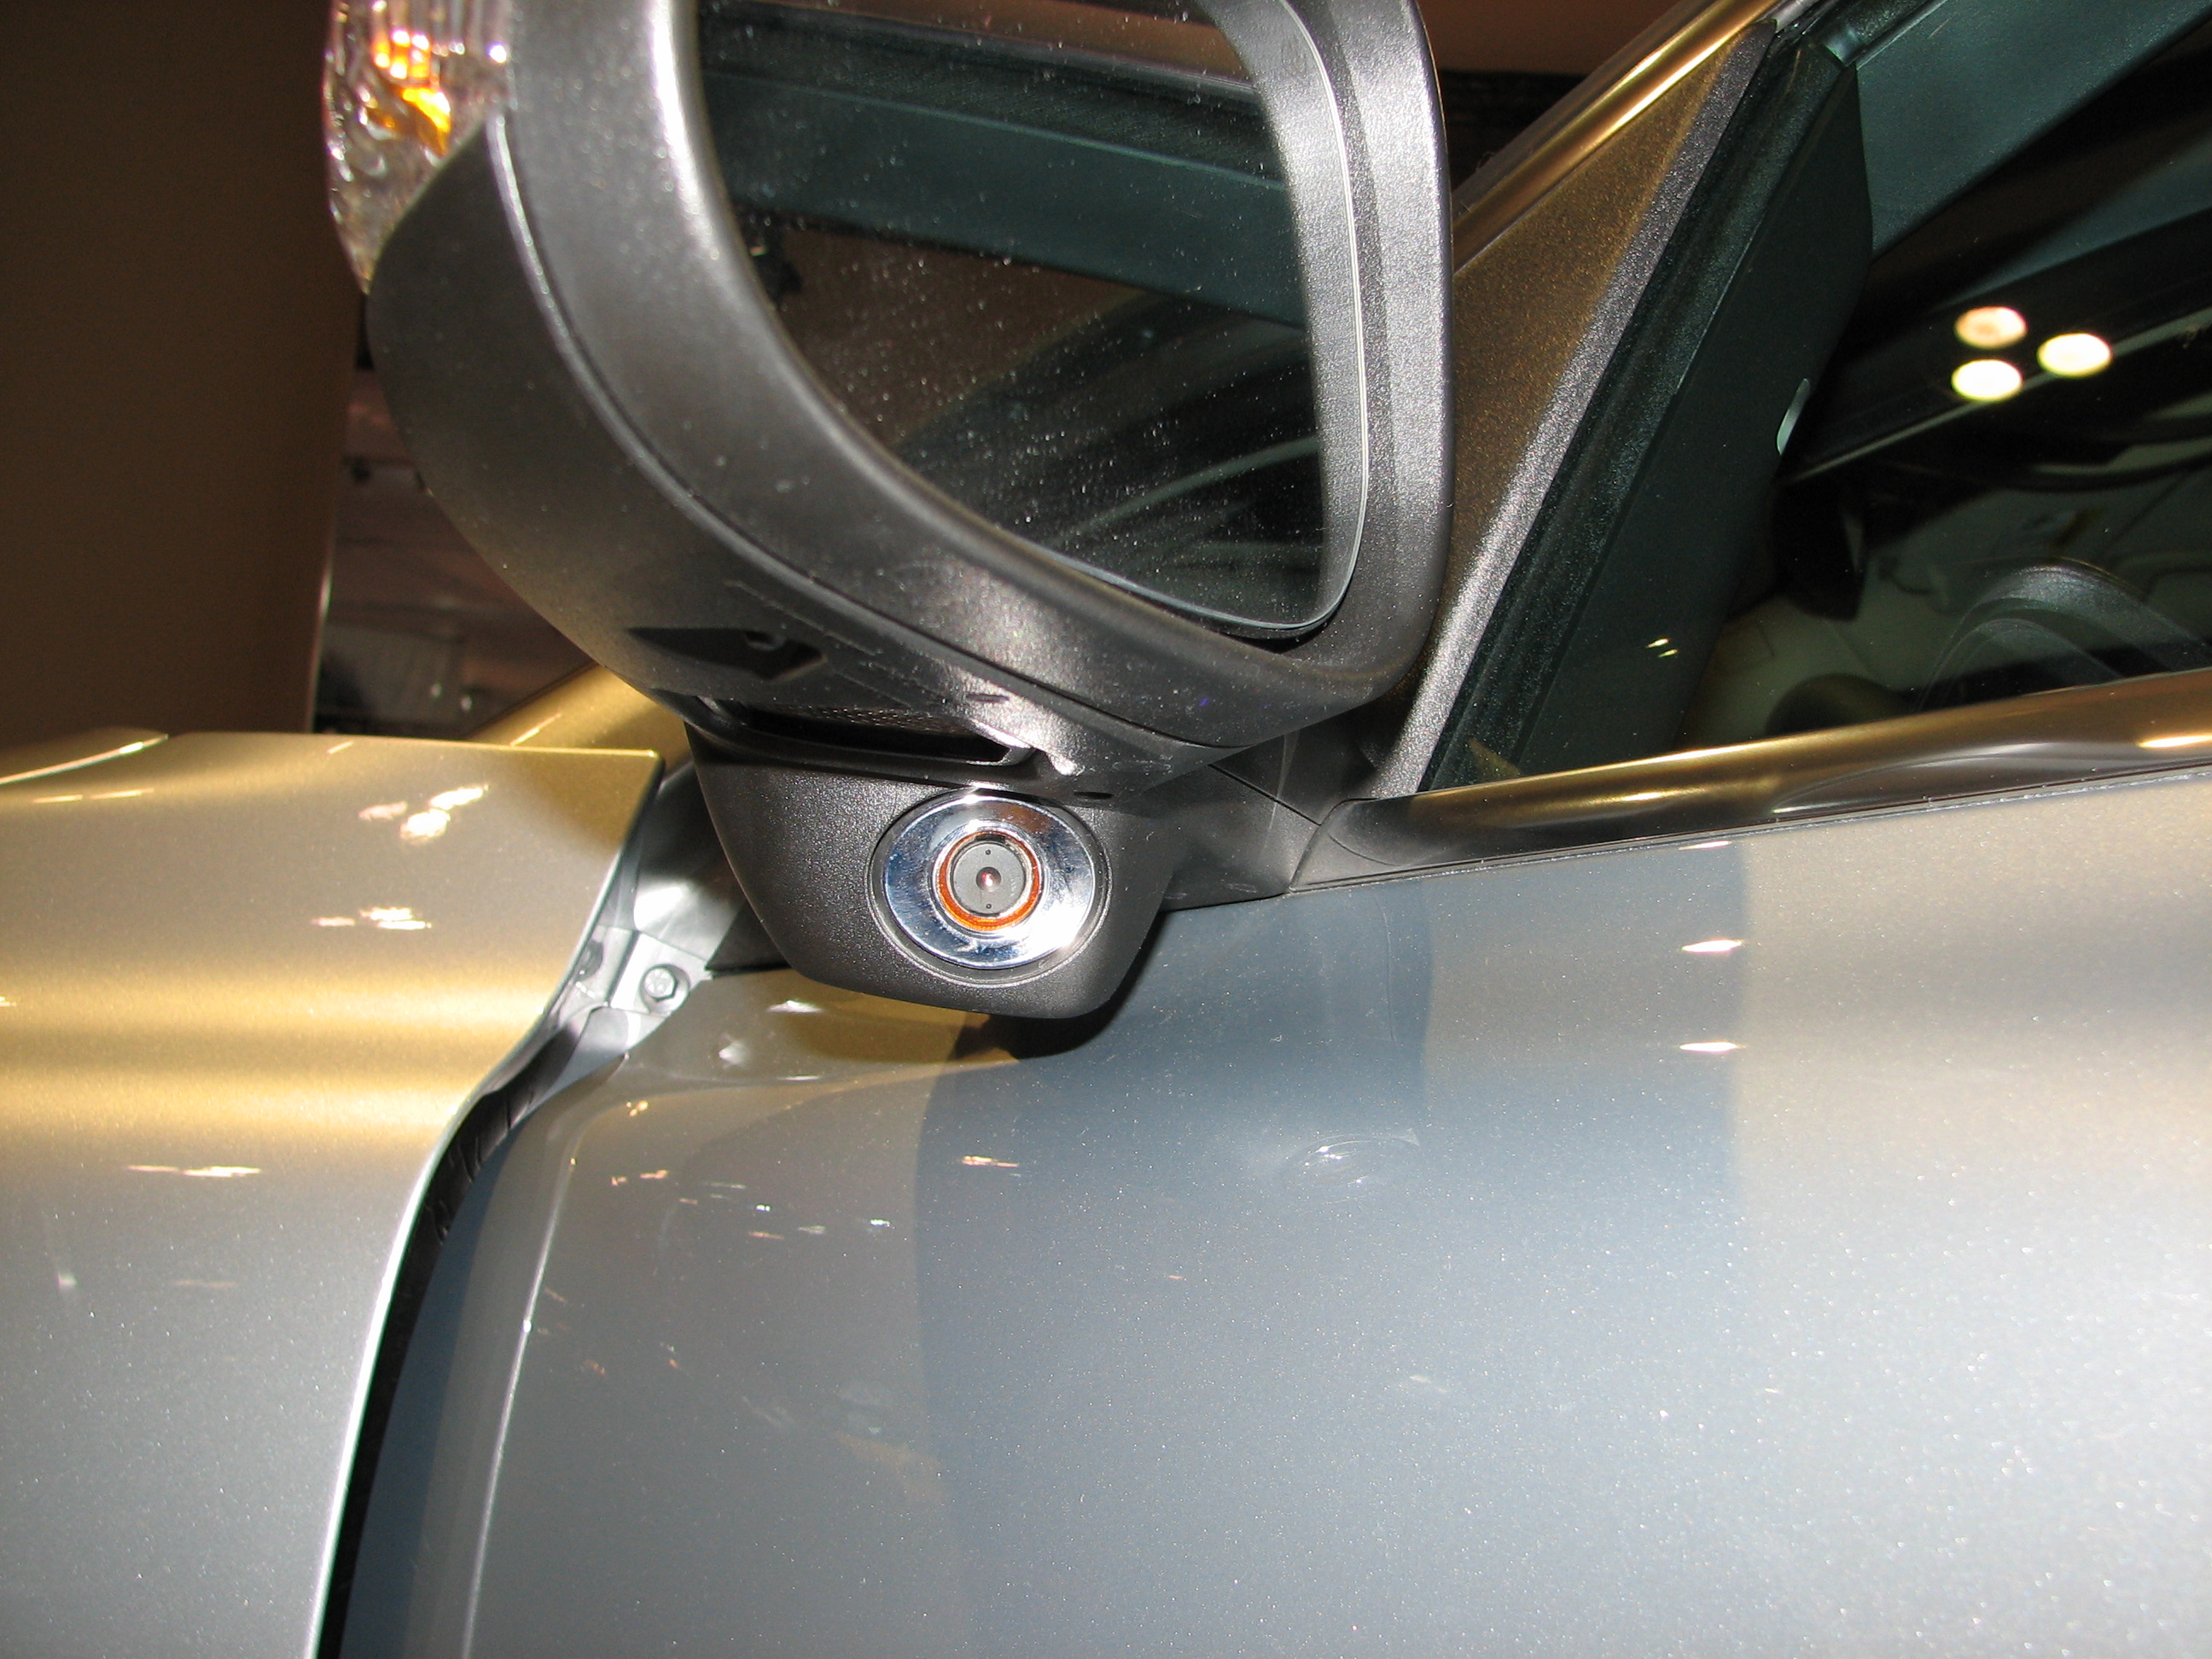
\includegraphics[scale=0.1]{figures/research_report/Volvo_BLIS}
\caption{Volvo's early camera based blind spot technology}
\end{figure}

When this system identifies a potential problem vehicle it notifies the driver using an led in the A-pillar (between the windscreen and door). This is very subtle which has both advantages and disadvantages. The main advantage being that it is unlikely to be annoying for the user, whereas a more active warning (i.e. a beeping) might be. However, the subtlety means that it is up to the driver to be checking whether the light is on - an extra check that they need to carry out before every manoeuvre.

More recent versions of this product now use a radar sensor in the rear of the car which allows it to check for crossing traffic when performing reversing manoeuvres \cite{volvo_radar}.

\subsubsection{Ford}
Ford have developed their own version of the BLIS system. Ford's system works using two radar sensors mounted on each corner of the rear bumper \cite{ford_blis}. The Ford system actually appears to be very similar to the Volvo one; the notification however is done in a slightly different way. Ford have incorporated the notification light into the wing mirrors; this has the slight advantage that the driver is likely to be checking these mirrors anyway before moving and so doesn't mean they have to check somewhere else before manoeuvring. However it still has the problem that the system is not very forceful about giving the warning and so it may be easy for more careless drivers to miss the warning all together. 

\subsubsection{Infiniti}
A more advanced system has been developed by Infiniti; they separate the system into two parts:
\begin{itemize}
\item Blind Spot Warning \cite{infiniti_warning}
\item Blind Spot Intervention \cite{infiniti_intervene}
\end{itemize}
The warning system is actually quite similar to the previous systems that we looked at but they do have a different approach to notifying the driver. Once the driver indicates to move into a blocked lane there will be an audible warning to the driver. We think that this may be a slightly better approach because it caters for those people who may not take the time to check their mirrors thoroughly and is much more difficult to miss. Also an audible warning is actually likely to be much more appropriate for any similar system implemented on a bike (because there are no mirrors).

It is after this where the system gets really clever, the intervention technology kicks in. The idea of the intervention technology is that if the driver continues to move towards the obstacle in their blind spot the intervention system will actually intervene to stop a collision from occurring. It intervenes by carefully applying braking on one side of the vehicle in order guide it back to the centre of the lane.

Something similar to the Blind Spot Intervention technology could be a potential consideration for use on a bike using braking in a similar way.
\subsection{Self driving cars}
Self driving cars are the pinnacle of car technology, although a long way from consumer release significant progress has been made in recent years. Self driving cars are essentially a combination of navigation systems, collision avoidance and automated driving systems. It is highly possible that a road full of self driving cars could reduce accidents down to almost none, by taking out the human error. This also shows what could be possible for bike technology.

However, when fully analysed it is clear that many of the technologies may not be possible to implement on a bicycle because of the way a bicycle is controlled. Cars are much more stable than bikes because of their four wheels and their power coming from a controllable engine. Bikes only have two wheels which means they are much more sensitive to sudden changes in their control and are powered via pedals which are very hard to manage. 

It may be possible to take the best elements of self driving cars and adapt them to fit into a bicycle setup - this would likely need to be an electric bike.
\subsection{Central Tire Inflation}
An actually quite old technology is Central Tire Inflation - here the idea is the tires can be inflated or deflated by a central device allowing the vehicle to work much more effectively in different road conditions. This device could be user controlled allowing them to change tire pressure centrally, but could also be connected to a series of sensors allowing them to monitor the road conditions and change the tire pressure accordingly. This has been heavily used in off-roading vehicles where the road conditions can change rapidly, but not so much in road vehicles. \cite{ctis} 

An attempt has been made to implement this technology on a bicycle\cite{ctis_bike} which could be potentially useful since bikes are particularly sensitive to road conditions, however it could well be the case that bikes are more sensitive to things like pot holes which this system would not really be able to help with.
\newpage
\section{Other research}
\subsection{Route planning}
Looking more deeply into route planning we realised that in order to incorporate it into our final solution we would need some method for determining the relative safety of any given road/route.

\subsubsection{User Perception}
One way to do this is to try and to model a cyclist's perception of the roads they cycle on. An attempt at this is the Bicycle Compatibility Index (BCI) \cite{bci-manual}; an American idea from 1998 as part of an initiative to double number of trips made by cycling or walking and to simultaneously reduce accidents by 10\%. The BCI is intended to be a measure of how well suited any particular road is to accommodate both motorists and cyclists.

The BCI was developed using the perspectives of cyclists; asking them to view videoclips and evaluate how comfortable they would be cycling on that road in the conditions shown. The index is then calculated using the method show in in figure \ref{fig:bci_calc}.
\begin{figure}[h]
\centering
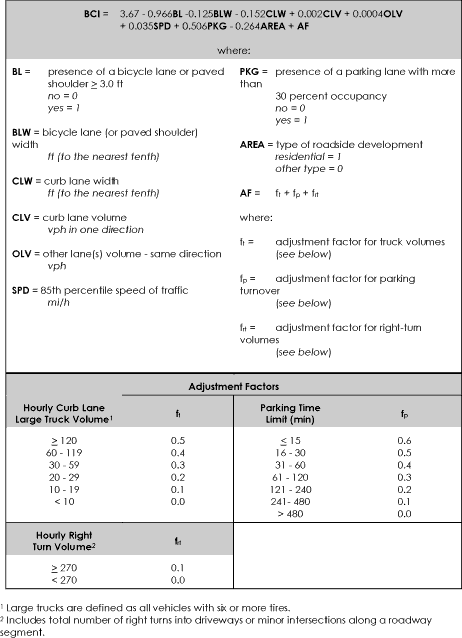
\includegraphics[scale=0.5]{figures/research_report/bci}
\caption{The calculation for the Bicycle Compatibility Index}
\label{fig:bci_calc}
\end{figure}

Fairly obviously, the presence of a dedicated cycle lane wider than 0.9m is the most significant factor on the comfort of cyclists, along with the width of the inside lane and cycle lanes. Interestingly though, according to the research, the speed of traffic is considered more important (0.022) than the volume of traffic (0.002); this would indicate that it would be better for cyclists to travel on gridlocked busy roads during rush hour rather than the back streets which although quieter are more likely to have traffic flowing faster.

The BCI also gives an indication towards what an index value means regarding how compatible the road is, this is shown in figure \ref{fig:bci_los}:

\begin{figure}[h]
\centering
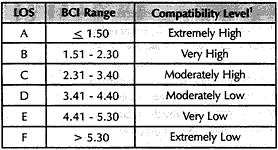
\includegraphics[scale=0.7]{figures/research_report/bci_los}
\caption{The 'Level of Service' designations for the BCI}
\label{fig:bci_los}
\end{figure}

\chapter{Stakeholder Map}
\label{ch:stakeholders}
On the following pages is a stakeholder map and analysis showing all of the people who may be affected by this project. 

Some of the stakeholders shown are directly affected, cyclists for example. Whereas others are only affected as a secondary effect.

Some may be positively affected by the project and other negatively. In the analysis we will show the likely reactions of some of the key holders and the reasons for this reaction.
\newpage
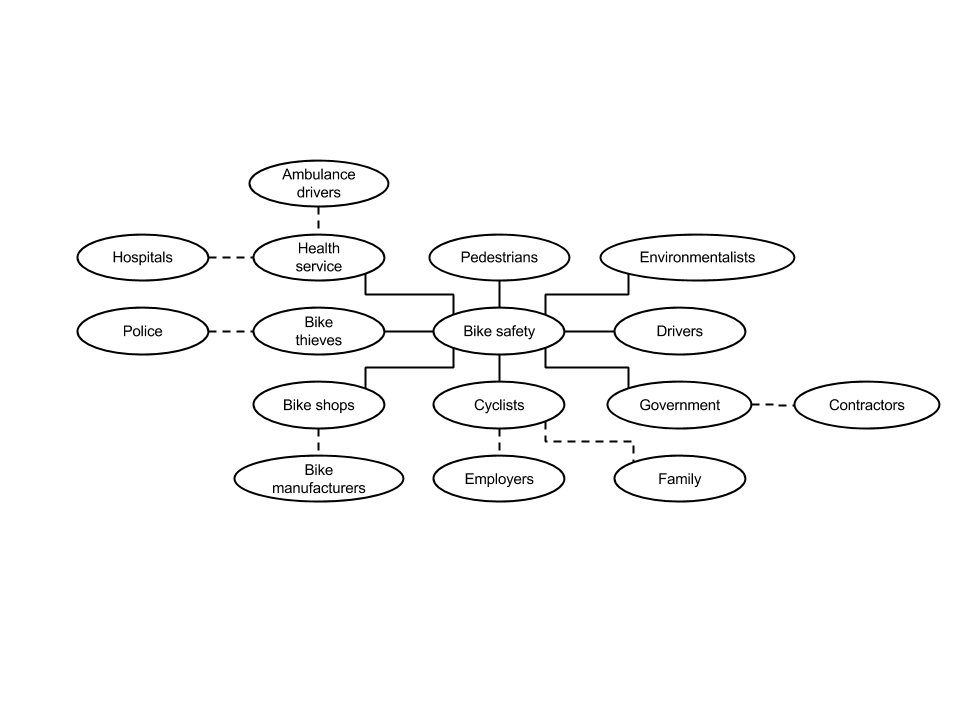
\includegraphics[scale=0.7, angle=90]{figures/stakeholder_map}
\newpage
\begin{center}
\begin{tabularx}{\linewidth}{|c|X|X|c|X|}
\hline
\textbf{Stakeholder} & \textbf{Goals} & \textbf{Behaviour} & \textbf{-ve or +ve?} & \textbf{Likely Reaction} \\ \hline
Bike shops & To sell bikes & Helpful, supportive & +ve & Promote the bike \\ \hline
Cyclists & To commute via bike & Supportive & +ve & Possibly purchase the bike or purchase other bikes as a result of safety in numbers \\ \hline
Drivers & To commute & Unhelpful and destructive & -ve & Strongly resist. Drivers in general definitely do not want an increase of cycling numbers \\ \hline
Pedestrians & To commute/get around & Unhelpful & -ve & Probably resist slightly since some cyclists have reputation for riding on pavement, running red lights, etc.  \\ \hline
Environmentalists & To protect the environment & Helpful, supportive & +ve & Would strongly support anything that leads to a reduction in CO2 emissions\\ \hline
Health service & To provide healthcare to the public & Helpful, supportive & +ve & Mixed. Would support increase in cycling as it is generally healthy. May worry about increased severity accidents\\ \hline
Bike Thieves & To make money from the theft of bicycles & Silently supportive & +ve & Would be happy about the prospect of more expensive bikes on the market \\ \hline
Government & To provide overall management to the transport system & Mixed & +ve & Mixed. Some areas of government would probably appreciate more cyclists on the road. However, an increased number of cyclists could lead to increased pressure to build cycle lanes and further infrastructure\\ \hline
\end{tabularx}
\end{center}

\chapter{Braking System}
\section{Research}

\begin{table}[h]

    \begin{tabular}{ | c | c |}
    \hline
    \textbf{Condition} & \textbf{Rolling Friction Coefficient (mm)} \\ \hline
   
   Bicycle tire on wooden track & 0.001   \\ \hline
   Bicycle tire on concrete & 0.002 \\ \hline
  Bicycle tire on asphalt road & 0.004 \\ \hline
  Bicycle tire on rough paved road & 0.008 \\ \hline

  \end{tabular}

\caption[Table caption text]{Bicycle Rolling Resistance for differing conditions \cite{cite:bicycle_friction}} 
\label{table:bicycle_friction}
\end{table}

\section{Early Sketches}
\label{app:early_sketches}

\begin{figure}[h]
\centering
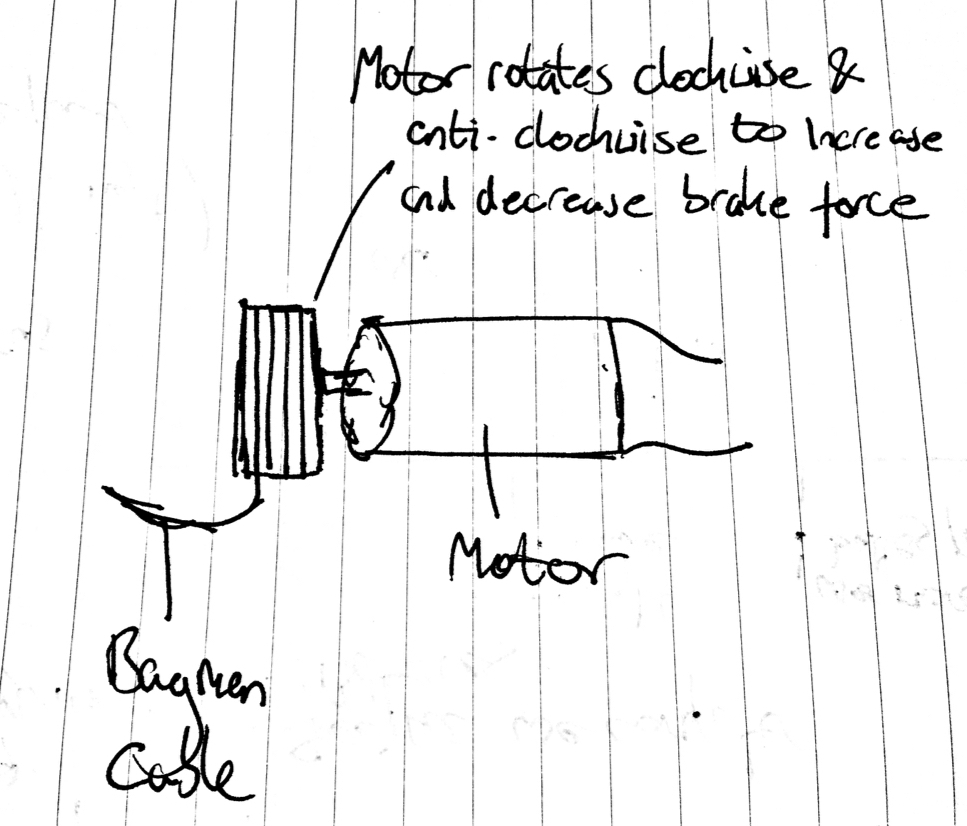
\includegraphics[scale=0.25]{figures/early_sketches/braking_system/motor_cable_tension}
\caption{Early design sketch using a motor to increase and decrease the tension of a bayman cable for use in the bicycle braking system}
\label{fig:early_motor_cable_tension}
\end{figure}

\section{Current Technology}
\label{app:brakes_current_technology}
\begin{figure}[h]
\centering
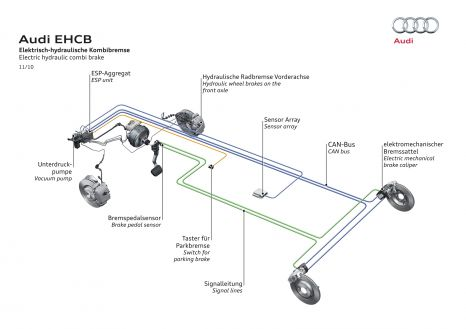
\includegraphics[scale=0.7]{figures/electronic_braking/audi_EHCB_1}
\caption{  \citep{audi_ehcb_1}}
\label{fig:audi_EHCB_1}
\end{figure}

\begin{figure}[h]
\centering
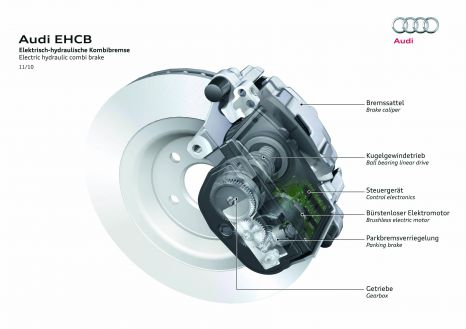
\includegraphics[scale=0.7]{figures/electronic_braking/audi_EHCB_2}
\caption{Audi Electric Hydraulic combo Brakes  \citep{audi_ehcb_2}}
\label{fig:audi_EHCB_2}
\end{figure}

\begin{figure}[h]
\centering
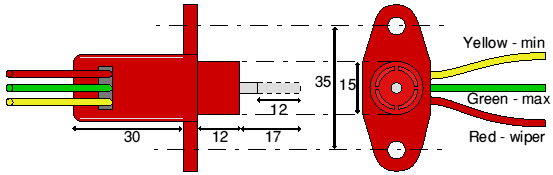
\includegraphics[scale=0.7]{figures/electronic_braking/spring_pot}
\caption{Spring operated potentiometer \citep{spring_pot}}
\label{fig:spring_pot}
\end{figure}

\begin{figure}[h]
\centering
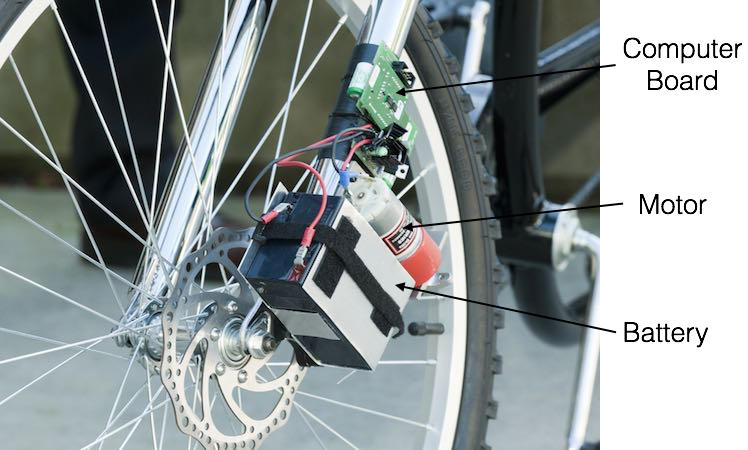
\includegraphics[scale=0.5]{figures/electronic_braking/wireless_bicycle_brakes_labelled}
\caption{Labelled Prototype of wireless by Pro Hermanns \citep{wireless_bicycle_brakes}}
\label{fig:wireless_bicycle_brakes}
\end{figure}

\chapter{Prototype 1}
\begin{figure}
\centering
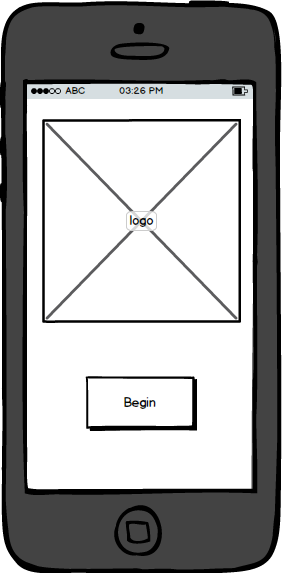
\includegraphics[scale=0.9]{figures/prototype_1/title}
\caption{Title screen}
\end{figure}
\clearpage
\begin{figure}
\centering
\includegraphics[scale=0.9]{figures/prototype_1/main_menu}
\caption{Main menu}
\end{figure}
\clearpage
\begin{figure}
\centering
\includegraphics[scale=0.9]{figures/prototype_1/locked}
\caption{Screen that displays when bike is locked}
\end{figure}
\clearpage
\begin{figure}
\centering
\includegraphics[scale=0.9]{figures/prototype_1/settings}
\caption{Screen allowing the user to adjust settings}
\end{figure}
\clearpage
\begin{figure}
\centering
\includegraphics[scale=0.9]{figures/prototype_1/settings_help_1}
\caption{Alert box explain what the setting does}
\end{figure}
\clearpage
\begin{figure}
\centering
\includegraphics[scale=0.9]{figures/prototype_1/settings_help_2}
\caption{Alert box explain what the setting does}
\end{figure}
\clearpage
\begin{figure}
\centering
\includegraphics[scale=0.9]{figures/prototype_1/settings_help_3}
\caption{Alert box explain what the setting does}
\end{figure}
\clearpage
\begin{figure}
\centering
\includegraphics[scale=0.9]{figures/prototype_1/settings_2}
\caption{Some more settings}
\end{figure}
\clearpage
\begin{figure}
\centering
\includegraphics[scale=0.9]{figures/prototype_1/settings_2_check}
\caption{Dropdown menu}
\end{figure}
\clearpage
\begin{figure}
\centering
\includegraphics[scale=0.9]{figures/prototype_1/factory_settings}
\caption{Warning when performing a factory reset}
\end{figure}
\clearpage
\begin{figure}
\centering
\includegraphics[scale=0.9]{figures/prototype_1/perf}
\caption{The performance screen. This is the main riding screen}
\end{figure}
\clearpage
\begin{figure}
\centering
\includegraphics[scale=0.9]{figures/prototype_1/reset_perf}
\caption{Warning when resetting performance stats}
\end{figure}
\clearpage
\begin{figure}
\centering
\includegraphics[scale=0.9]{figures/prototype_1/resetted}
\caption{The performance screen following a reset}
\end{figure}
\clearpage
\begin{figure}
\centering
\includegraphics[scale=0.9]{figures/prototype_1/brake_maint}
\caption{A brake maintenance alert, this could display over any screen}
\end{figure}
\clearpage
\begin{figure}
\centering
\includegraphics[scale=0.9]{figures/prototype_1/main_menu_warn}
\caption{The main menu showing the warning icon at the top}
\end{figure}
\clearpage
\begin{figure}
\centering
\includegraphics[scale=0.8]{figures/prototype_1/collision_activate}
\caption{Warning explaining collision detection system before it is de/activated}
\end{figure}
\clearpage
\begin{figure}
\centering
\includegraphics[scale=0.9]{figures/prototype_1/collision_on}
\caption{Main menu screen showing that collision detection is on}
\end{figure}
\clearpage
\begin{figure}
\centering
\includegraphics[scale=0.8]{figures/prototype_1/control_alert_perf}
\caption{Alert showing that the collision detection system has started to take control. Could display on any screen}
\end{figure}
\clearpage
\begin{figure}
\centering
\includegraphics[scale=0.9]{figures/prototype_1/inflation_settings}
\caption{Alert showing that automatic tire-inflation has been activated. Could display on any screen}
\end{figure}
\clearpage
\begin{figure}
\centering
\includegraphics[scale=0.9]{figures/prototype_1/settings_saved}
\caption{Alert showing that the updated settings have been saved}
\end{figure}
\clearpage

\chapter{Prototype 2}
\begin{figure}
\centering
\includegraphics[scale=0.9]{figures/prototype_2/title}
\caption{Title screen}
\end{figure}
\clearpage
\begin{figure}
\centering
\includegraphics[scale=0.9]{figures/prototype_2/not_paired}
\caption{Message prompting the user to pair the phone with a bicycle}
\end{figure}
\clearpage
\begin{figure}
\centering
\includegraphics[scale=0.9]{figures/prototype_2/already_reg}
\caption{This message will display when the device is paired with a brand new bicycle - it has no master user}
\end{figure}
\clearpage
\begin{figure}
\centering
\includegraphics[scale=0.9]{figures/prototype_2/reg_warn}
\caption{There can only be one master user for a bicycle so there is a warning telling users they are about to set the master user}
\end{figure}
\clearpage
\begin{figure}
\centering
\includegraphics[scale=0.9]{figures/prototype_2/no_conn_master}
\caption{An internet connection is needed to perform the initial setup - registering as a master user of a bike}
\end{figure}
\clearpage
\begin{figure}
\centering
\includegraphics[scale=0.9]{figures/prototype_2/startup}
\caption{Startup screen allowing users to either login or register}
\end{figure}
\clearpage
\begin{figure}
\centering
\includegraphics[scale=0.9]{figures/prototype_2/connecting}
\caption{Showing the status of the device - connecting to the server}
\end{figure}
\clearpage
\begin{figure}
\centering
\includegraphics[scale=0.9]{figures/prototype_2/connect_err}
\caption{Error message displaying when the device could not connect to the server}
\end{figure}
\clearpage
\begin{figure}
\centering
\includegraphics[scale=0.9]{figures/prototype_2/unrecognised_err}
\caption{Error message displaying the user credentials could not be located on the database}
\end{figure}
\clearpage
\begin{figure}
\centering
\includegraphics[scale=0.9]{figures/prototype_2/unrecognised_warn}
\caption{If the user logs in with valid credentials but they are not a registed user of the bike in question they will not be allowed access until the master user adds them}
\end{figure}
\clearpage
\begin{figure}
\centering
\includegraphics[scale=0.9]{figures/prototype_2/create_success}
\caption{Message telling the user that they have successfully created a new account}
\end{figure}
\clearpage
\begin{figure}
\centering
\includegraphics[scale=0.9]{figures/prototype_2/pass_conf_err}
\caption{Error message telling the user why their account could not be created}
\end{figure}
\clearpage
\begin{figure}
\centering
\includegraphics[scale=0.9]{figures/prototype_2/missing_err}
\caption{General error message telling users they must fill in all boxes. Could be incorporated with other features (highlighting missing boxes, etc.)}
\end{figure}
\clearpage
\begin{figure}
\centering
\includegraphics[scale=0.9]{figures/prototype_2/offline_warn}
\caption{Users will be able to cycle without an internet connection however they may not be able to save changes to their settings}
\end{figure}
\clearpage
\begin{figure}
\centering
\includegraphics[scale=0.9]{figures/prototype_2/main}
\caption{Main menu}
\end{figure}
\clearpage
\begin{figure}
\centering
\includegraphics[scale=0.9]{figures/prototype_2/accounts}
\caption{The master user will be able to use this screen to change the registered users of the bike}
\end{figure}
\clearpage
\begin{figure}
\centering
\includegraphics[scale=0.9]{figures/prototype_2/add_user_warn}
\caption{Warning, explaining that adding a user gives them control over the bike when they want it}
\end{figure}
\clearpage
\begin{figure}
\centering
\includegraphics[scale=0.9]{figures/prototype_2/add_user}
\caption{Screen to enter the new bike users credentials}
\end{figure}
\clearpage\begin{figure}
\centering
\includegraphics[scale=0.9]{figures/prototype_2/account_added}
\caption{A user is successfully registered with the bike}
\end{figure}
\clearpage
\begin{figure}
\centering
\includegraphics[scale=0.9]{figures/prototype_2/add_user_conn}
\caption{Connecting to the server to find the new user}
\end{figure}
\clearpage
\begin{figure}
\centering
\includegraphics[scale=0.9]{figures/prototype_2/add_user_err_conn}
\caption{It is not possible to add a user without an internet connection}
\end{figure}
\clearpage\begin{figure}
\centering
\includegraphics[scale=0.9]{figures/prototype_2/add_user_unrecognised}
\caption{If the user could not be found}
\end{figure}
\clearpage
\begin{figure}
\centering
\includegraphics[scale=0.9]{figures/prototype_2/add_user_boxes_err}
\caption{Error message if user fills out the form incorrectly}
\end{figure}
\clearpage
\begin{figure}
\centering
\includegraphics[scale=0.9]{figures/prototype_2/locked}
\caption{Screen that displays when bike is locked}
\end{figure}
\clearpage
\begin{figure}
\centering
\includegraphics[scale=0.9]{figures/prototype_2/settings}
\caption{Screen allowing the user to adjust settings}
\end{figure}
\clearpage
\begin{figure}
\centering
\includegraphics[scale=0.9]{figures/prototype_2/settings_help_1}
\caption{Alert box explain what the setting does}
\end{figure}
\clearpage
\begin{figure}
\centering
\includegraphics[scale=0.9]{figures/prototype_2/settings_help_2}
\caption{Alert box explain what the setting does}
\end{figure}
\clearpage
\begin{figure}
\centering
\includegraphics[scale=0.9]{figures/prototype_2/settings_help_3}
\caption{Alert box explain what the setting does}
\end{figure}
\clearpage
\begin{figure}
\centering
\includegraphics[scale=0.9]{figures/prototype_2/settings_2}
\caption{Some more settings}
\end{figure}
\clearpage
\begin{figure}
\centering
\includegraphics[scale=0.9]{figures/prototype_2/settings_2_check}
\caption{Dropdown menu}
\end{figure}
\clearpage
\begin{figure}
\centering
\includegraphics[scale=0.9]{figures/prototype_2/factory_reset}
\caption{Warning when performing a factory reset}
\end{figure}
\clearpage
\begin{figure}
\centering
\includegraphics[scale=0.9]{figures/prototype_2/performance}
\caption{The performance screen. This is the main riding screen}
\end{figure}
\clearpage
\begin{figure}
\centering
\includegraphics[scale=0.9]{figures/prototype_2/performance_reset}
\caption{Warning when resetting performance stats}
\end{figure}
\clearpage
\begin{figure}
\centering
\includegraphics[scale=0.9]{figures/prototype_2/performance_resetted}
\caption{The performance screen following a reset}
\end{figure}
\clearpage
\begin{figure}
\centering
\includegraphics[scale=0.9]{figures/prototype_2/brake_maintenance}
\caption{A brake maintenance alert, this could display over any screen}
\end{figure}
\clearpage
\begin{figure}
\centering
\includegraphics[scale=0.9]{figures/prototype_2/main_brake_warn}
\caption{The main menu showing the warning icon at the top}
\end{figure}
\clearpage
\begin{figure}
\centering
\includegraphics[scale=0.8]{figures/prototype_2/collision_activate}
\caption{Warning explaining collision detection system before it is de/activated}
\end{figure}
\clearpage
\begin{figure}
\centering
\includegraphics[scale=0.9]{figures/prototype_2/main_collision}
\caption{Main menu screen showing that collision detection is on}
\end{figure}
\clearpage
\begin{figure}
\centering
\includegraphics[scale=0.8]{figures/prototype_2/performance_control_alert}
\caption{Alert showing that the collision detection system has started to take control. Could display on any screen}
\end{figure}
\clearpage
\begin{figure}
\centering
\includegraphics[scale=0.8]{figures/prototype_2/main_control_alert}
\caption{Alert showing that the collision detection system has started to take control. Could display on any screen}
\end{figure}
\clearpage
\begin{figure}
\centering
\includegraphics[scale=0.8]{figures/prototype_2/settings_control_alert}
\caption{Alert showing that the collision detection system has started to take control. Could display on any screen}
\end{figure}
\clearpage
\begin{figure}
\centering
\includegraphics[scale=0.9]{figures/prototype_2/settings_connection_warn}
\caption{Without an internet connection changes to settings will be saved locally, but it is possible that they will get lost}
\end{figure}
\clearpage
\begin{figure}
\centering
\includegraphics[scale=0.9]{figures/prototype_2/settings_saved}
\caption{Alert showing that the updated settings have been saved}
\end{figure}
\clearpage
\begin{figure}
\centering
\includegraphics[scale=0.9]{figures/prototype_2/map}
\caption{Basic map screen so that users can get routing information from Google Maps}
\end{figure}
\clearpage

  
\bibliographystyle{plainnat}
\bibliography{bibliography}
 

\end{document}
